\documentclass[13pt,a4paper,oneside]{extreport}
\usepackage[utf8]{inputenc}
\usepackage[T5]{fontenc}
\usepackage[vietnamese]{babel}
\usepackage{mathptmx} % Times New Roman
\usepackage{graphicx}
\usepackage{tabularx}
\usepackage{multirow}
\usepackage{caption}
\usepackage{subcaption}
\usepackage{amsmath,amssymb}
\usepackage{titlesec}
\usepackage{setspace}
\usepackage{fancyhdr}
\usepackage{tocloft}
\usepackage{indentfirst}
\usepackage[top=3cm, bottom=3cm, left=3cm, right=2cm]{geometry}
\usepackage[unicode]{hyperref}
\usepackage{cite}
\usepackage{tikz}

% Nạp thông tin đồ án tập trung (tên đề tài, tác giả, chuyên ngành, năm,...)
% ==============================================================================
% THÔNG TIN ĐỒ ÁN TỐT NGHIỆP (CẤU HÌNH TẬP TRUNG TOÀN BỘ THÔNG SỐ)
% ==============================================================================
% Sau này chỉ cần chỉnh sửa tại file này, toàn bộ Bìa ngoài, Bìa phụ, Tóm tắt,
% Lời cam đoan, Lời cảm ơn và Nội dung sẽ tự động cập nhật đồng bộ 100%.

% ------------------------------------------------------------------------------
% 1. TÊN ĐỀ TÀI (Đề tài chính thức: Tiếng Việt)
% ------------------------------------------------------------------------------
\newcommand{\tendetai}{Hệ thống Hỏi đáp và Gợi ý Lịch trình Du lịch Thông minh dựa trên Đồ thị Tri thức Không gian và Mô hình Ngôn ngữ Lớn}

% Tên đề tài ngắt dòng cân xứng trên trang Bìa ngoài và Bìa phụ (size lớn)
\newcommand{\tendetaiBia}{Hệ thống Hỏi đáp và Gợi ý Lịch trình\\ Du lịch Thông minh dựa trên Đồ thị Tri thức\\ Không gian và Mô hình Ngôn ngữ Lớn}

% Bản dịch tiếng Anh chính thức
\newcommand{\tendetaiTiengAnh}{Smart Tourism Q\&A and Itinerary Recommendation System based on Spatial Knowledge Graphs and Large Language Models}
\newcommand{\tendetaiTiengAnhBia}{Smart Tourism Q\&A and Itinerary\\ Recommendation System based on Spatial\\ Knowledge Graphs and Large Language Models}

% ------------------------------------------------------------------------------
% 2. THÔNG TIN SINH VIÊN VÀ NGƯỜI HƯỚNG DẪN
% ------------------------------------------------------------------------------
\newcommand{\sinhvien}{LÊ HOÀNG MINH QUÝ}
\newcommand{\mssv}{22E1020017}
\newcommand{\nguoihuongdan}{TS. Hồ Quốc Dũng}

% ------------------------------------------------------------------------------
% 3. THÔNG TIN KHOA, BỘ MÔN VÀ CHUYÊN NGÀNH
% ------------------------------------------------------------------------------
\newcommand{\tentruong}{ĐẠI HỌC HUẾ}
\newcommand{\tenkhoa}{KHOA KỸ THUẬT VÀ CÔNG NGHỆ}
\newcommand{\tenbomon}{BỘ MÔN KHOA HỌC DỮ LIỆU VÀ TRÍ TUỆ NHÂN TẠO}
\newcommand{\tenchuyennganh}{KHOA HỌC DỮ LIỆU VÀ TRÍ TUỆ NHÂN TẠO}
\newcommand{\tenchuyennganhBia}{KHOA HỌC DỮ LIỆU\\ VÀ TRÍ TUỆ NHÂN TẠO}
\newcommand{\loaihinhdoan}{KHÓA LUẬN TỐT NGHIỆP ĐẠI HỌC}

% ------------------------------------------------------------------------------
% 4. ĐỊA ĐIỂM VÀ NĂM HOÀN THÀNH
% ------------------------------------------------------------------------------
\newcommand{\diadiemnam}{THÀNH PHỐ HUẾ, NĂM 2026}
\newcommand{\thanhpho}{TP Huế}
\newcommand{\namtotnghiep}{2026}


% Cài đặt giãn dòng 1.5 lines
\setstretch{1.5}

% Cài đặt khoảng cách giữa các đoạn 6pt và thụt đầu dòng 1cm
\setlength{\parskip}{6pt}
\setlength{\parindent}{1cm}

% Định dạng phân cấp cỡ chữ chuẩn học thuật (thân bài 13pt): 16pt -> 14pt -> 13pt
% Yêu cầu bắt buộc: Mọi cấp số hiệu (Chương 1.), (1.1.), (1.2.), (1.2.1.) phải kết thúc bằng dấu chấm (.)
\titleformat{\chapter}[hang]
  {\normalfont\fontsize{16pt}{20pt}\selectfont\bfseries\centering}{\chaptertitlename\ \thechapter.}{0.5em}{\fontsize{16pt}{20pt}\selectfont}

\titleformat{name=\chapter,numberless}[hang]
  {\normalfont\fontsize{16pt}{20pt}\selectfont\bfseries\centering}{}{0pt}{\fontsize{16pt}{20pt}\selectfont}

\titleformat{\section}
  {\normalfont\fontsize{14pt}{18pt}\selectfont\bfseries\itshape}{\thesection.}{1em}{}

\titleformat{\subsection}
  {\normalfont\fontsize{13pt}{17pt}\selectfont\bfseries\itshape}{\thesubsection.}{1em}{}

\titleformat{\subsubsection}
  {\normalfont\fontsize{13pt}{17pt}\selectfont\itshape}{\thesubsubsection.}{1em}{}

% Thu gọn khoảng hở trên/dưới cho toàn bộ tiêu đề chương và mục
\titlespacing*{\chapter}{0pt}{15pt}{12pt}
\titlespacing*{name=\chapter,numberless}{0pt}{15pt}{12pt}
\titlespacing*{\section}{0pt}{12pt}{6pt}
\titlespacing*{\subsection}{0pt}{10pt}{4pt}
\titlespacing*{\subsubsection}{0pt}{8pt}{3pt}

% Cấu hình Mục lục (tocloft) chuẩn HUET Mẫu 6: có dấu chấm kết thúc số hiệu và in nghiêng từ cấp 2 đến cấp 4
\renewcommand{\cftchapleader}{\normalfont\cftdotfill{\cftchapdotsep}}
\renewcommand{\cftchappresnum}{Chương }
\renewcommand{\cftchapaftersnum}{.}
\setlength{\cftchapnumwidth}{2.4cm}

\renewcommand{\cftsecfont}{\itshape}
\renewcommand{\cftsecaftersnum}{.}
\setlength{\cftsecnumwidth}{1.2cm}
\setlength{\cftsecindent}{0.8cm}

\renewcommand{\cftsubsecfont}{\itshape}
\renewcommand{\cftsubsecaftersnum}{.}
\setlength{\cftsubsecnumwidth}{1.5cm}
\setlength{\cftsubsecindent}{1.5cm}

\renewcommand{\cftsubsubsecfont}{\itshape}
\renewcommand{\cftsubsubsecaftersnum}{.}
\setlength{\cftsubsubsecnumwidth}{1.8cm}
\setlength{\cftsubsubsecindent}{2.2cm}

% Đổi tên các danh mục in hoa chuẩn HUET Mẫu 6, 8, 9
\addto\captionsvietnamese{%
  \renewcommand{\contentsname}{MỤC LỤC}%
  \renewcommand{\listtablename}{DANH MỤC CÁC BẢNG, BIỂU}%
  \renewcommand{\listfigurename}{DANH MỤC CÁC SƠ ĐỒ, ĐỒ THỊ, HÌNH VẼ}%
  \renewcommand{\bibname}{TÀI LIỆU THAM KHẢO}%
}

% Căn giữa và đồng bộ 16pt in đậm cho tiêu đề Mục lục, Danh mục Bảng, Danh mục Hình (ghi đè mặc định của tocloft)
\renewcommand{\cfttoctitlefont}{\hfill\normalfont\fontsize{16pt}{20pt}\selectfont\bfseries}
\renewcommand{\cftaftertoctitle}{\hfill}

\renewcommand{\cftlottitlefont}{\hfill\normalfont\fontsize{16pt}{20pt}\selectfont\bfseries}
\renewcommand{\cftafterlottitle}{\hfill}

\renewcommand{\cftloftitlefont}{\hfill\normalfont\fontsize{16pt}{20pt}\selectfont\bfseries}
\renewcommand{\cftafterloftitle}{\hfill}

% Lệnh định dạng PHẦN chuẩn HUET Mẫu 6 (đồng bộ 16pt, in hoa, in đậm, căn giữa)
\newcommand{\phan}[1]{%
  \clearpage
  \phantomsection
  \vspace*{-0.5cm}%
  {\centering\normalfont\fontsize{16pt}{20pt}\selectfont\bfseries #1\par}%
  \vspace{0.5cm}%
  \addcontentsline{toc}{chapter}{#1}%
}

% Cài đặt Header & Footer
\pagestyle{fancy}
\fancyhf{}
\renewcommand{\headrulewidth}{0pt}
\fancyfoot[C]{\thepage} % Đánh số trang ở giữa phía dưới

\begin{document}

% Các trang bìa ngoài và bìa phụ (không đánh số trang)
\begin{titlepage}
\thispagestyle{empty}
\newgeometry{top=2.1cm, bottom=2.1cm, left=2.7cm, right=1.6cm}

% Hệ thống khung viền theo Mẫu 1 (gồm Cột gáy sách và Khung mặt bìa chính)
\begin{tikzpicture}[remember picture, overlay]
  % Cột gáy sách bên trái (chuẩn Mẫu 1 bìa cứng)
  \draw[line width=1pt] 
    ([xshift=1.2cm, yshift=-2.0cm]current page.north west) 
    rectangle 
    ([xshift=2.2cm, yshift=2.0cm]current page.south west);

  % Dòng chữ trên gáy sách (in hoa, xoay dọc từ trên xuống dưới theo Mẫu 1)
  \node[rotate=-90, font=\fontsize{10pt}{12pt}\selectfont\bfseries, anchor=center] 
    at ([xshift=1.7cm]current page.west) 
    {\sinhvien\ -- \loaihinhdoan\ -- \tenchuyennganh\ -- HUẾ \namtotnghiep};

  % Khung viền chính bao quanh mặt bìa
  \draw[line width=1.5pt] 
    ([xshift=2.5cm, yshift=-2.0cm]current page.north west) 
    rectangle 
    ([xshift=-1.5cm, yshift=2.0cm]current page.south east);
\end{tikzpicture}

\begin{center}
\vspace*{-0.9cm} % Đẩy chữ ĐẠI HỌC HUẾ sát ngay cạnh trên của khung viền chuẩn bản gốc

% Khối 1: Trường - Khoa - Bộ môn (sát ngay mép khung trên)
{\fontsize{14pt}{18pt}\selectfont \MakeUppercase{\tentruong}} \\[0.2cm]
{\fontsize{14pt}{18pt}\selectfont \bfseries \MakeUppercase{\tenkhoa}} \\[0.2cm]
{\fontsize{14pt}{18pt}\selectfont \bfseries \MakeUppercase{\tenbomon}}\\[-0.3cm]
\rule{3cm}{0.8pt} \\[0.4cm]

% Khối 2: Biểu trưng (Logo) HUET

\includegraphics[width=4.5cm]{img/logo-huet-300x300.png} \\[1cm]

% Khối 3: Họ và tên sinh viên (size 14, in đậm)
{\fontsize{14pt}{18pt}\selectfont \bfseries \MakeUppercase{\sinhvien}}

\vspace*{\stretch{0.1}}

% Khối 4: Tên đề tài (size 24, in đậm, ngắt 3 dòng cân xứng ở trung tâm trang)
{\fontsize{24pt}{32pt}\selectfont \bfseries \MakeUppercase{\tendetaiBia}\par}

\vspace*{\stretch{0.5}}

% Khối 5: Khóa luận / Đồ án tốt nghiệp & Tên chuyên ngành (size 24, liền một khối thống nhất)
{\fontsize{24pt}{30pt}\selectfont \bfseries \MakeUppercase{\loaihinhdoan}\par}
{\fontsize{24pt}{30pt}\selectfont \bfseries \MakeUppercase{\tenchuyennganhBia}\par}

\vfill

% Khối 6: Địa điểm và năm báo cáo (sát mép dưới khung viền theo Mẫu 1)
{\fontsize{14pt}{18pt}\selectfont \bfseries \diadiemnam}
\vspace*{-0.2cm}

\end{center}
\restoregeometry
\end{titlepage}

\begin{titlepage}
\thispagestyle{empty}
\newgeometry{top=2.1cm, bottom=2.1cm, left=3.0cm, right=2.0cm}

% Khung viền bao quanh toàn bộ trang bìa phụ theo Mẫu 2
\begin{tikzpicture}[remember picture, overlay]
  \draw[line width=1.5pt] 
    ([xshift=3.0cm, yshift=-2.0cm]current page.north west) 
    rectangle 
    ([xshift=-2.0cm, yshift=2.0cm]current page.south east);
\end{tikzpicture}

\begin{center}
\vspace*{-0.9cm} % Đẩy chữ ĐẠI HỌC HUẾ sát ngay cạnh trên của khung viền chuẩn bản gốc

% Khối 1: Trường - Khoa - Bộ môn (sát ngay mép khung trên)
{\fontsize{14pt}{18pt}\selectfont \MakeUppercase{\tentruong}} \\[0.2cm]
{\fontsize{14pt}{18pt}\selectfont \bfseries \MakeUppercase{\tenkhoa}} \\[0.2cm]
{\fontsize{14pt}{18pt}\selectfont \bfseries \MakeUppercase{\tenbomon}}\\[-0.3cm]
\rule{3cm}{0.8pt} \\[0.4cm]

% Khối 2: Biểu trưng (Logo) HUET (kích thước lớn 4.5cm như bìa ngoài)

\includegraphics[width=4.5cm]{img/logo-huet-300x300.png} \\[1cm]

% Khối 3: Họ và tên sinh viên – Mã số sinh viên (size 14, in đậm)
{\fontsize{14pt}{18pt}\selectfont \bfseries \MakeUppercase{\sinhvien\ -- \mssv}}

\vspace*{\stretch{0.1}}

% Khối 4: Tên đề tài (size 22, in đậm, ngắt 3 dòng cân xứng)
{\fontsize{22pt}{29pt}\selectfont \bfseries \MakeUppercase{\tendetaiBia}\par}

\vspace*{\stretch{0.5}}

% Khối 5: Khóa luận / Đồ án tốt nghiệp & Tên chuyên ngành (size 20, liền một khối thống nhất)
{\fontsize{20pt}{26pt}\selectfont \bfseries \MakeUppercase{\loaihinhdoan}\par}
{\fontsize{20pt}{26pt}\selectfont \bfseries \MakeUppercase{\tenchuyennganhBia}\par}

\vfill

% Khối 6: Cụm Người hướng dẫn (căn giữa)
{\fontsize{14pt}{18pt}\selectfont Người hướng dẫn:} \\[0.2cm]
{\fontsize{14pt}{18pt}\selectfont \bfseries \nguoihuongdan}

\vfill

% Khối 7: Địa điểm và năm báo cáo (sát mép dưới khung viền theo Mẫu 2)
{\fontsize{14pt}{18pt}\selectfont \bfseries \diadiemnam}
\vspace*{-0.2cm}

\end{center}
\restoregeometry
\end{titlepage}


% Các trang trước phần mở đầu đánh số La Mã, bắt đầu từ trang i theo Mẫu 6
\pagenumbering{roman}
\setcounter{page}{1}

\chapter*{LỜI CAM ĐOAN}
\addcontentsline{toc}{chapter}{LỜI CAM ĐOAN}

Tôi xin cam đoan đây là công trình nghiên cứu của riêng tôi và được sự hướng dẫn khoa học của \nguoihuongdan.

Các nội dung nghiên cứu, kết quả trong đề tài này là trung thực và chưa công bố dưới bất kỳ hình thức nào trước đây. Những số liệu trong các bảng biểu phục vụ cho việc phân tích, nhận xét, đánh giá được chính tác giả thu thập từ các nguồn khác nhau có ghi rõ trong phần tài liệu tham khảo.

Ngoài ra, trong \loaihinhdoan\ còn sử dụng một số nhận xét, đánh giá cũng như số liệu của các tác giả khác, cơ quan tổ chức khác đều có trích dẫn và chú thích nguồn gốc.

Nếu phát hiện có bất kỳ sự gian lận nào tôi xin hoàn toàn chịu trách nhiệm về nội dung \loaihinhdoan\ của mình. Khoa Kỹ thuật và Công nghệ - Đại học Huế không liên quan đến những vi phạm tác quyền, bản quyền do tôi gây ra trong quá trình thực hiện (nếu có).

\vspace{1.5cm}
\begin{flushright}
\thanhpho, ngày \dots tháng \dots năm \namtotnghiep\ \\
\textbf{SINH VIÊN} \\
\textit{(Ký, ghi rõ họ tên)} \\[1.5cm]
\textbf{\sinhvien}
\end{flushright}

\chapter*{LỜI CẢM ƠN}
\addcontentsline{toc}{chapter}{LỜI CẢM ƠN}

Trước tiên, tôi xin bày tỏ lòng biết ơn sâu sắc nhất tới \textbf{\nguoihuongdan}, người đã luôn tận tình hướng dẫn, định hướng khoa học và động viên tôi trong suốt quá trình nghiên cứu và hoàn thành khóa luận tốt nghiệp này.

Tôi cũng xin gửi lời cảm ơn chân thành đến quý Thầy, Cô giáo tại Khoa Kỹ thuật và Công nghệ - Đại học Huế đã truyền đạt những kiến thức quý báu và tạo điều kiện học tập tốt nhất cho tôi trong suốt thời gian học tập tại trường.

Cuối cùng, tôi xin gửi lời cảm ơn tới gia đình và bạn bè đã luôn đồng hành, chia sẻ và tiếp thêm động lực cho tôi trong suốt quá trình học tập và nghiên cứu.

\vspace{1.5cm}
\begin{flushright}
\thanhpho, ngày \dots tháng \dots năm \namtotnghiep\ \\
\textbf{SINH VIÊN} \\
\textit{(Ký, ghi rõ họ tên)} \\[1.5cm]
\textbf{\sinhvien}
\end{flushright}

\clearpage
\phantomsection
\addcontentsline{toc}{chapter}{TÓM TẮT}

\begin{center}
% 1. TÊN ĐỀ TÀI Ở TRÊN (Size 14, in hoa, in đậm) theo Mẫu 5
{\fontsize{14pt}{18pt}\selectfont \bfseries \MakeUppercase{\tendetai}\par}
\vspace{0.6cm}

% 2. TÓM TẮT Ở DƯỚI (Size 14, in hoa, in đậm) theo Mẫu 5
{\fontsize{14pt}{18pt}\selectfont \bfseries TÓM TẮT\par}
\vspace{0.8cm}
\end{center}

Trong kỷ nguyên chuyển đổi số và phát triển du lịch thông minh, việc ứng dụng các Mô hình Ngôn ngữ Lớn (Large Language Models -- LLM) nhằm hỗ trợ du khách tra cứu thông tin và tự động thiết kế lịch trình tham quan ngày càng trở nên phổ biến. Mặc dù sở hữu năng lực tạo sinh ngôn ngữ tự nhiên vượt trội, các hệ thống LLM thương mại độc lập cùng các kiến trúc Tăng cường Tạo sinh Truy xuất truyền thống (Naive RAG) thường xuyên bộc lộ hai rào cản kỹ thuật nghiêm trọng khi đối mặt với dữ liệu du lịch địa phương: hiện tượng ảo giác thực thể (Entity Hallucination) dẫn đến việc tự bịa đặt các địa danh không có thật, và sự thiếu hụt nhận thức không gian (Space-agnostic limitation) sinh ra các lịch trình di chuyển ziczac, vi phạm cự ly đi lại thực tế và chia cắt địa hình tự nhiên (như hai bờ sông Hương tại Cố đô Huế).

Khóa luận này đề xuất và hiện thực hóa một giải pháp tích hợp toàn diện mang tên Spatial GraphRAG, kết hợp chặt chẽ giữa Đồ thị Tri thức Không gian (Spatial Knowledge Graph gồm 9.525 nút thực thể và 90.948 cạnh quan hệ), kho dữ liệu đánh giá du khách quy mô lớn (1,69 triệu bài nhận xét từ TripAdvisor), và khung điều phối tác tử tự suy ngẫm (Agentic RAG) trên nền tảng LangGraph vận hành hoàn toàn cục bộ bằng mô hình Qwen2.5-3B trên máy trạm cá nhân (Zero API Cost). Đồng thời, đề tài xây dựng bộ từ điển ẩm thực 570 món ăn phục vụ khai phá thực đơn ngầm và phát triển giải thuật lập lịch trình phân cụm địa lý (Spatial Itinerary Planner) kết nối cổng API RESTful chuẩn mở sẵn sàng tích hợp với nền tảng công dân số Hue-S.

Kết quả kiểm thử thực nghiệm trên bộ benchmark 12 kịch bản du lịch thực tế tại Huế khẳng định mô hình Spatial GraphRAG đạt tỷ lệ bảo chứng thực thể tuyệt đối (Grounding Rate 100\%), triệt tiêu hoàn toàn tỷ lệ ảo giác và lỗi vi phạm cự ly (0\% Spatial Violation), rút ngắn khoảng cách di chuyển trung bình xuống 1,25~km (so với 4,5~km của Naive RAG và 6,8~km của Zero-shot LLM), đồng thời nâng độ chính xác món ăn đặc sản lên 96,5\% với thời gian đáp ứng thời gian thực 2,8 giây.


\phantomsection
\addcontentsline{toc}{chapter}{MỤC LỤC}
\tableofcontents

\clearpage
\phantomsection
\addcontentsline{toc}{chapter}{DANH MỤC CÁC CHỮ VIẾT TẮT VÀ KÝ HIỆU}

\begin{center}
{\fontsize{14pt}{18pt}\selectfont \bfseries DANH MỤC CÁC CHỮ VIẾT TẮT VÀ KÝ HIỆU\par}
\vspace{0.8cm}
\end{center}

\noindent
\begin{tabularx}{\textwidth}{l l X}
\hline
\textbf{Ký hiệu} & \textbf{Tiếng Anh} & \textbf{Ý nghĩa tiếng Việt} \\
\hline
AI & Artificial Intelligence & Trí tuệ nhân tạo \\
API & Application Programming Interface & Giao diện lập trình ứng dụng \\
CLIP & Contrastive Language-Image Pretraining & Tiền huấn luyện tương phản Ngôn ngữ -- Hình ảnh \\
DS\&AI & Data Science \& Artificial Intelligence & Khoa học Dữ liệu và Trí tuệ Nhân tạo \\
GPS & Global Positioning System & Hệ thống định vị toàn cầu \\
GPU & Graphics Processing Unit & Bộ xử lý đồ họa \\
HUET & Hue University of Engineering and Technology & Khoa Kỹ thuật và Công nghệ -- Đại học Huế \\
JSON & JavaScript Object Notation & Định dạng trao đổi dữ liệu đối tượng \\
JWT & JSON Web Token & Chuẩn mở định dạng mã thông báo bảo mật \\
KG & Knowledge Graph & Đồ thị tri thức \\
LLM & Large Language Model & Mô hình ngôn ngữ lớn \\
LOOCV & Leave-One-Out Cross-Validation & Kiểm định chéo loại từng phần tử \\
NLP & Natural Language Processing & Xử lý ngôn ngữ tự nhiên \\
NoSQL & Not Only SQL & Mô hình cơ sở dữ liệu phi quan hệ \\
OAuth & Open Authorization & Khung ủy quyền phân tán tiêu chuẩn mở \\
OP & Orienteering Problem & Bài toán định tuyến định hướng có giới hạn \\
OSM & OpenStreetMap & Dự án bản đồ số mở toàn cầu \\
OSRM & Open Source Routing Machine & Hệ thống tính toán định tuyến mã nguồn mở \\
POI & Point of Interest & Điểm tham quan / Điểm dịch vụ du lịch \\
RAG & Retrieval-Augmented Generation & Tạo sinh tăng cường truy xuất \\
REST & Representational State Transfer & Phong cách kiến trúc mạng hướng dịch vụ \\
RLHF & Reinforcement Learning from Human Feedback & Học tăng cường từ phản hồi của con người \\
RWD & Responsive Web Design & Thiết kế web đáp ứng đa kích thước màn hình \\
SKG & Spatial Knowledge Graph & Đồ thị tri thức không gian \\
TTDP & Tourist Trip Design Problem & Bài toán thiết kế chuyến đi du lịch \\
ViT & Vision Transformer & Mô hình mạng biến đổi thị giác \\
VRAM & Video Random Access Memory & Bộ nhớ truy cập ngẫu nhiên của bộ xử lý đồ họa \\
WMO & World Meteorological Organization & Tổ chức Khí tượng Thế giới \\
XAI & Explainable Artificial Intelligence & Trí tuệ nhân tạo có thể giải thích được \\
\hline
\end{tabularx}

\phantomsection
\addcontentsline{toc}{chapter}{DANH MỤC CÁC BẢNG, BIỂU}
\listoftables

\phantomsection
\addcontentsline{toc}{chapter}{DANH MỤC CÁC SƠ ĐỒ, ĐỒ THỊ, HÌNH VẼ}
\listoffigures


% Phần nội dung chính (đánh số Ả Rập từ trang 1 của Phần I)
\pagenumbering{arabic}
\setcounter{page}{1}

\phan{PHẦN I. PHẦN MỞ ĐẦU}
\label{phan:mo-dau}

\section*{1. Tính cấp thiết của đề tài}
\addcontentsline{toc}{section}{1. Tính cấp thiết của đề tài}

Thừa Thiên Huế là trung tâm văn hóa, lịch sử và du lịch đặc sắc hàng đầu của Việt Nam, sở hữu Quần thể Di tích Cố đô Huế được UNESCO vinh danh là Di sản Văn hóa Thế giới cùng hệ thống lăng tẩm triều Nguyễn, danh lam cổ tự và nền văn hóa ẩm thực cung đình lẫn dân gian trứ danh. Trong tiến trình xây dựng và phát triển tỉnh Thừa Thiên Huế trở thành thành phố trực thuộc Trung ương theo định hướng tại Nghị quyết số 54-NQ/TW của Bộ Chính trị, nhiệm vụ đẩy mạnh chuyển đổi số ngành du lịch và xây dựng hệ sinh thái đô thị thông minh đóng vai trò là đòn bẩy phát triển kinh tế xã hội trọng điểm. Cùng với sự bùng nổ của các mô hình ngôn ngữ lớn (Large Language Models -- LLM) và trí tuệ nhân tạo tạo sinh, hành vi của du khách hiện đại đã có sự chuyển biến căn bản: người dùng ngày càng có nhu cầu tương tác với các trợ lý ảo đàm thoại thông minh có khả năng thấu hiểu ngữ cảnh tự nhiên, tư vấn lịch trình cá nhân hóa, gợi ý địa điểm ẩm thực địa phương chuẩn xác và tối ưu hóa tuyến đường theo thời gian thực thay vì tra cứu thủ công qua các danh bạ tĩnh truyền thống.

Tuy nhiên, trong thực tiễn công tác quản lý và xúc tiến du lịch tại địa phương, ngành du lịch Thừa Thiên Huế đang đứng trước bài toán chiến lược mang tính sống còn về việc kéo dài thời gian lưu trú và gia tăng mức chi tiêu của du khách. Vấn đề cấp bách này đã được lãnh đạo Thành phố Huế đặc biệt nhấn mạnh trong chuyến khảo sát thực địa và chỉ đạo điều hành vào tháng 9 năm 2026, được cơ quan báo chí phản ánh rộng rãi, tiêu biểu như bài viết trên Báo Thanh Niên~\cite{thanhnien2026tourism} được ghi nhận tại Hình~\ref{fig:thanhnien-tourism}.

\begin{figure}[htbp]
    \centering
    
\includegraphics[width=0.88\textwidth]{img/thanhnien_hue_tourism_problem.png}
    \caption{Bài báo phản ánh chỉ đạo của lãnh đạo thành phố Huế về yêu cầu giải quyết ba câu hỏi cốt lõi của du khách: Đi đâu, ăn gì, lưu trú ở đâu trên Báo Thanh Niên~\cite{thanhnien2026tourism}.}
    \label{fig:thanhnien-tourism}
\end{figure}

Từ nội dung chỉ đạo thực tế được phản ánh trên Hình~\ref{fig:thanhnien-tourism}, lãnh đạo chính quyền Thành phố Huế sau các chuyến kiểm tra thực địa tại chợ Đông Ba, các không gian kết nối phát triển phố đêm và tuyến đường đi dạo ven sông Như Ý đã triệu tập cuộc họp chuyên đề nhằm tìm kiếm các giải pháp đột phá. Thông điệp cốt lõi được đặt ra cho toàn ngành du lịch Cố đô là: \textit{Huế phải trả lời một cách thỏa đáng, tức thời và thuyết phục ba câu hỏi căn bản của du khách: Đi đâu? Ăn gì? Lưu trú ở đâu?}. Nếu không giải quyết thấu đáo chuỗi nhu cầu liên hoàn này, du khách sẽ chỉ đến Huế theo hình thức tham quan chớp nhoáng ban ngày rồi di chuyển sang các địa phương lân cận, khiến ngành du lịch địa phương bỏ lỡ nguồn doanh thu dịch vụ và kinh tế đêm to lớn.

Nhằm hiện thực hóa mục tiêu chuyển đổi số phục vụ người dân và du khách, tỉnh Thừa Thiên Huế đã tiên phong xây dựng nền tảng đô thị thông minh Hue-S~\cite{hues2024}, tích hợp phân hệ thông tin du lịch và dịch vụ công dân số. Dù đạt được nhiều thành tựu quan trọng về mặt chính quyền điện tử, khi đi sâu vào phân hệ hỗ trợ du lịch tương tác, ứng dụng Hue-S hiện tại vẫn bộc lộ những hạn chế kỹ thuật đáng kể, được minh họa trực quan thông qua hai giao diện thực tế tại Hình~\ref{fig:hues-analysis}.

\begin{figure}[htbp]
    \centering
    \begin{subfigure}[b]{0.47\textwidth}
        \centering
        
\includegraphics[width=\textwidth]{img/hues_smart_city_app_home.png}
        \caption{Giao diện chính phân hệ du lịch trên Hue-S}
        \label{subfig:hues-home}
    \end{subfigure}
    \hfill
    \begin{subfigure}[b]{0.47\textwidth}
        \centering
        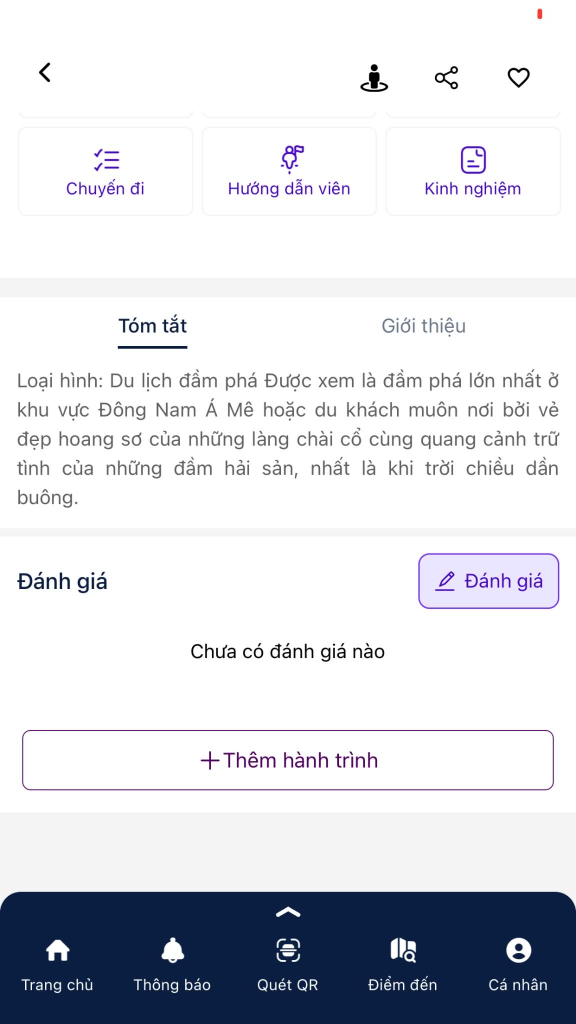
\includegraphics[width=\textwidth]{img/hues_app_limitation_review.png}
        \caption{Chi tiết điểm đến bộc lộ hạn chế đánh giá và lập lịch}
        \label{subfig:hues-detail}
    \end{subfigure}
    \caption{Thực trạng giao diện phân hệ du lịch trên nền tảng đô thị thông minh Hue-S cho thấy sự thiếu vắng dữ liệu đánh giá thực tế và công cụ lập lịch trình tự động~\cite{hues2024}.}
    \label{fig:hues-analysis}
\end{figure}

Quan sát giao diện thực tế tại Hình~\ref{subfig:hues-home}, phân hệ du lịch của Hue-S hiện tại hoạt động theo mô hình cổng thông tin điện tử một chiều: cung cấp thanh tìm kiếm từ khóa cơ bản, thông tin thời tiết, quảng bá dịch vụ vé tàu di sản tuyến Huế -- Đà Nẵng và danh mục các điểm đến phân theo nhóm thiên nhiên hoặc di tích. Tuy nhiên, khi người dùng truy cập sâu vào chi tiết của một địa danh du lịch (như điểm đến du lịch đầm phá Tam Giang -- Cầu Hai trên Hình~\ref{subfig:hues-detail}), hệ thống bộc lộ hai rào cản trải nghiệm hết sức rõ rệt. Thứ nhất, tại mục \textit{Đánh giá}, hệ thống thông báo trạng thái \textit{``Chưa có đánh giá nào''}. Điều này phản ánh thực trạng thiếu hụt trầm trọng cơ sở dữ liệu phản hồi thực tế từ cộng đồng du khách (Cold-start Review Gap), thiếu vắng các thuật toán phân tích cảm xúc (Sentiment Analysis) và hoàn toàn không có khả năng khai phá thị hiếu ẩm thực hay các món ăn đặc sản được yêu thích tại địa phương. Thứ hai, nút bấm chức năng \textit{Thêm hành trình} chỉ đóng vai trò như một danh sách đánh dấu (bookmark) thủ công thụ động. Người dùng phải tự tìm kiếm địa điểm, tự căn chỉnh cự ly và tự ước lượng thời gian di chuyển mà không nhận được bất kỳ sự hỗ trợ nào từ thuật toán tối ưu hóa tuyến đường có nhận thức không gian (Spatial Routing Engine).

Để giải quyết khoảng trống giữa kỳ vọng của du khách và năng lực của các ứng dụng du lịch hiện hành, xu hướng ứng dụng trí tuệ nhân tạo tạo sinh mở ra tiềm năng lớn. Dẫu vậy, việc áp dụng trực tiếp các mô hình ngôn ngữ lớn thương mại hoặc các hệ thống Tăng cường Tạo sinh Truy xuất truyền thống (Naive RAG) vào miền du lịch địa phương tại Huế đang vấp phải ba thách thức kỹ thuật cốt lõi:

Thách thức thứ nhất xuất phát từ hiện tượng ảo giác thực thể địa phương (Local Entity Hallucination). Do dữ liệu tiền huấn luyện của các mô hình LLM chủ yếu dựa trên ngữ liệu tổng quát toàn cầu, mô hình thường xuyên tự bịa đặt tên các quán ăn, nhà hàng nghe có vẻ giống tiếng Việt nhưng hoàn toàn không tồn tại trong thực tế tại Huế, hoặc gán ghép sai lệch giữa đặc sản các vùng miền. Tình trạng này làm suy giảm nghiêm trọng độ tin cậy của hệ thống tư vấn và có thể gây phương hại trực tiếp đến trải nghiệm thực địa của du khách.

Thách thức thứ hai là khiếm khuyết thiếu nhận thức không gian (Space-agnostic limitation). Bản chất của cơ chế tìm kiếm tương đồng véc-tơ trong Naive RAG thuần túy dựa trên sự tương đồng ngữ nghĩa văn bản mà hoàn toàn không nắm bắt được tọa độ địa lý, địa hình tự nhiên và cự ly di chuyển thực tế. Tại một đô thị có địa hình đặc thù bị chia cắt bởi dòng sông Hương như thành phố Huế, sự thiếu hụt này dẫn đến những lịch trình hết sức phi lý: hệ thống liên tục gợi ý du khách di chuyển ziczac qua lại giữa bờ Bắc (khu vực di sản Kinh thành) và bờ Nam (khu vực phố mới và các lăng tẩm), hoặc gợi ý các quán ăn cách xa điểm tham quan hàng chục kilômét trong khi du khách đang có nhu cầu đi bộ lân cận.

Thách thức thứ ba nằm ở sự chia cắt giữa dữ liệu đánh giá thực tế và cấu trúc biểu diễn tri thức. Thông tin đăng ký kinh doanh chính thống của các nhà hàng, quán ăn thường chỉ cung cấp danh mục chung chung, thiếu sự kiểm chứng về chất lượng thực tế. Trong khi đó, hàng chục ngàn bài nhận xét của du khách trên các nền tảng trực tuyến như TripAdvisor lại chứa đựng nguồn tri thức ngầm vô cùng phong phú về các món ăn đặc sản được yêu thích nhất tại từng địa điểm nhưng chưa được khai phá và liên kết có cấu trúc vào cơ sở tri thức.

Xuất phát từ những đòi hỏi thực tiễn của chính quyền thành phố Huế và khoảng trống học thuật nêu trên, đề tài \textbf{\tendetai} được đề xuất nhằm nghiên cứu và xây dựng một khung giải pháp toàn diện: tích hợp Đồ thị Tri thức Không gian (Spatial Knowledge Graph) với mô hình ngôn ngữ lớn cục bộ thông qua kiến trúc tác tử đa luồng (Agentic RAG). Giải pháp này hướng tới mục tiêu triệt tiêu ảo giác địa danh, tối ưu hóa cung đường di chuyển theo cụm địa lý và khai phá khẩu vị ẩm thực du khách, qua đó trả lời một cách tự động và chuẩn xác ba câu hỏi cốt lõi: Đi đâu, ăn gì và lưu trú ở đâu phục vụ đắc lực cho công tác quảng bá du lịch Cố đô Huế.

\section*{2. Mục tiêu nghiên cứu}
\addcontentsline{toc}{section}{2. Mục tiêu nghiên cứu}

Mục tiêu tổng quát của khóa luận là thiết kế, hiện thực hóa và đánh giá định lượng một hệ thống hỏi đáp và gợi ý lịch trình du lịch thông minh mang tên Spatial GraphRAG, kết hợp cấu trúc Đồ thị Tri thức Không gian, dữ liệu phản hồi thực tế của du khách và khung tác tử điều phối đa luồng trên nền tảng mô hình ngôn ngữ lớn cục bộ, nhằm cung cấp các đề xuất du lịch chuẩn xác về mặt thực thể và tối ưu về mặt cự ly địa lý tại thành phố Huế.

Để đạt được mục tiêu tổng quát, nghiên cứu xác lập bốn mục tiêu cụ thể.

Mục tiêu cụ thể thứ nhất là xây dựng Đồ thị Tri thức Không gian du lịch hoàn chỉnh cho Huế và các tỉnh thành trọng điểm với quy mô hơn 9.500 nút thực thể và hơn 90.000 cạnh quan hệ ngữ nghĩa, tích hợp thuộc tính tọa độ GPS chuẩn WGS84 và bán kính lân cận thực tế theo công thức khoảng cách mặt cầu Haversine.

Mục tiêu cụ thể thứ hai là xây dựng bộ từ điển ẩm thực Việt Nam gồm 570 món ăn (trong đó có hơn 60 món đặc sản Huế) và thiết lập giải thuật khai phá tri thức ngầm từ tập ngữ liệu 44.355 bài đánh giá du khách thực tế tại Huế trên nền tảng TripAdvisor để liên kết tự động quan hệ phục vụ món ăn vào đồ thị với độ tin cậy thống kê cao.

Mục tiêu cụ thể thứ ba là thiết kế khung điều phối Agentic RAG trên LangGraph tích hợp bộ chấm điểm tin cậy (Confidence Grading) và cơ chế phân luồng dự phòng tìm kiếm Internet, vận hành hoàn toàn trên mô hình ngôn ngữ mã nguồn mở cục bộ Qwen2.5-3B nhằm bảo đảm quyền riêng tư của du khách và triệt tiêu toàn bộ chi phí bản quyền API vận hành.

Mục tiêu cụ thể thứ tư là hiện thực hóa giải thuật lập lịch trình phân cụm địa lý (Spatial Itinerary Planner), phát triển giao diện Web tương tác bản đồ số trực quan và đóng gói Cổng API RESTful chuẩn mở sẵn sàng tích hợp với nền tảng công dân số Hue-S.

\section*{3. Câu hỏi nghiên cứu và Giả thuyết khoa học}
\addcontentsline{toc}{section}{3. Câu hỏi nghiên cứu và Giả thuyết khoa học}

Tiến trình nghiên cứu được định hướng bởi bốn câu hỏi nghiên cứu cốt lõi:

Câu hỏi nghiên cứu RQ1: Làm thế nào để mô hình hóa mối quan hệ không gian giữa các điểm tham quan, nhà hàng ẩm thực và cơ sở lưu trú thành một Đồ thị Tri thức Không gian có khả năng truy vấn hiệu quả theo bán kính địa lý thực tế?

Câu hỏi nghiên cứu RQ2: Cơ chế trích xuất thực đơn ngầm từ hàng chục ngàn bài đánh giá văn bản phi cấu trúc của du khách có thể nâng cao độ chính xác và độ phong phú của việc gợi ý món ăn đặc sản so với dữ liệu phân loại tĩnh truyền thống ở mức độ nào?

Câu hỏi nghiên cứu RQ3: Việc tích hợp Đồ thị Tri thức Không gian vào quy trình RAG (Spatial GraphRAG) có thể triệt tiêu hiện tượng ảo giác thực thể và giảm thiểu tỷ lệ vi phạm cự ly di chuyển so với Naive RAG và Zero-shot LLM ra sao?

Câu hỏi nghiên cứu RQ4: Khung tác tử LangGraph kết hợp mô hình ngôn ngữ cục bộ quy mô nhỏ (Qwen2.5-3B) có đáp ứng được yêu cầu về thời gian phản hồi thời gian thực và độ chính xác tổng thể khi vận hành trên hạ tầng máy trạm tiêu chuẩn hay không?

Tương ứng với các câu hỏi nghiên cứu nêu trên, khóa luận xác lập bốn giả thuyết khoa học:

Giả thuyết khoa học $H_1$: Ràng buộc topo không gian (cạnh liên kết lân cận trong bán kính mặt cầu $d \le 1,5\text{ km}$) sẽ triệt tiêu hoàn toàn các lộ trình ziczac nhảy bờ sông Hương vô lý, giảm cự ly di chuyển trung bình ít nhất 50\% so với hệ thống Naive RAG truyền thống.

Giả thuyết khoa học $H_2$: Khai phá thực đơn ngầm từ tập ngữ liệu nhận xét du khách cho phép mở rộng độ phủ món ăn đặc sản lên trên 90\%, vượt trội so với danh mục ẩm thực phân loại tĩnh.

Giả thuyết khoa học $H_3$: Mô hình Spatial GraphRAG đạt tỷ lệ bảo chứng thực thể (Grounding Rate) 100\% và tỷ lệ ảo giác địa danh 0\% trên toàn bộ các truy vấn kiểm thử thuộc phạm vi đồ thị tri thức.

Giả thuyết khoa học $H_4$: Quy trình phân cụm lịch trình theo không gian kết hợp bộ lập lịch trình thông minh bảo đảm thời gian sinh kết quả dưới 4 giây trên GPU cá nhân, hoàn toàn đủ điều kiện cung cấp dịch vụ trực tuyến ổn định trong điều kiện thực tế.

\section*{4. Đối tượng và Phạm vi nghiên cứu}
\addcontentsline{toc}{section}{4. Đối tượng và Phạm vi nghiên cứu}

Đối tượng nghiên cứu của khóa luận là các phương pháp biểu diễn tri thức không gian (Spatial Knowledge Representation), kỹ thuật Tăng cường Tạo sinh Truy xuất dựa trên đồ thị (GraphRAG), khung điều phối tác tử hội thoại thông minh (Agentic Workflows) và các giải thuật tối ưu hóa lịch trình du lịch dựa trên địa lý. Về mặt dữ liệu, đối tượng nghiên cứu bao gồm 9.525 thực thể điểm du lịch, ẩm thực, lưu trú và 44.355 bản ghi đánh giá du khách thực tế tại Huế thu thập từ TripAdvisor, kết hợp dữ liệu tọa độ hình học từ OpenStreetMap và Google Maps.

Về phạm vi nghiên cứu, không gian địa lý trọng tâm của đề tài được định vị tại thành phố Huế và các vùng phụ cận thuộc tỉnh Thừa Thiên Huế (khu vực Kinh thành, cụm lăng tẩm phía Nam, đầm Chuồn, đầm phá Tam Giang, làng cổ Phước Tích, cầu ngói Thanh Toàn). Các thực thể tại các tỉnh thành du lịch lân cận (Đà Nẵng, Quảng Nam) đóng vai trò làm giàu ngữ cảnh đồ thị liên kết vùng. Về mặt công nghệ, nghiên cứu tập trung vào mô hình ngôn ngữ cục bộ Qwen2.5-3B-Instruct vận hành qua môi trường Ollama trên GPU NVIDIA GeForce RTX 3050 (4GB VRAM), bảo đảm tính khả thi triển khai và vận hành tự chủ hoàn toàn tại các cơ quan, đơn vị địa phương.

\section*{5. Ý nghĩa khoa học và Thực tiễn}
\addcontentsline{toc}{section}{5. Ý nghĩa khoa học và Thực tiễn}

Về mặt khoa học, khóa luận đóng góp một khung phương pháp luận mới kết hợp giữa tính toán không gian (Spatial Computing) và GraphRAG. Nghiên cứu làm rõ cơ chế tích hợp khoảng cách mặt cầu Haversine vào cấu trúc đồ thị tri thức, đồng thời đề xuất giải pháp dung hợp giữa tri thức có cấu trúc của đồ thị và tri thức phi cấu trúc từ nhận xét du khách để định hướng quá trình suy luận của LLM mà không cần tái huấn luyện mô hình nền tảng.

Về mặt thực tiễn, sản phẩm của đề tài mang lại giá trị ứng dụng trực tiếp cho ngành du lịch Thừa Thiên Huế. Hệ thống không chỉ cung cấp giải pháp trợ lý ảo thông minh giúp du khách tự lập kế hoạch du lịch tiết kiệm thời gian và chi phí, mà còn sẵn sàng kết nối API vào nền tảng số Hue-S, hỗ trợ chính quyền địa phương giải quyết bài toán: Đi đâu, ăn gì, lưu trú ở đâu, điều tiết dòng khách du lịch hợp lý giữa các cụm di sản, góp phần bảo tồn di tích và thúc đẩy kinh tế đêm bền vững.

\section*{6. Cấu trúc của khóa luận}
\addcontentsline{toc}{section}{6. Cấu trúc của khóa luận}

Khóa luận được kết cấu thành năm phần theo đúng quy định tại Văn bản số 1967/HD-ĐHH của Đại học Huế:

Phần I trình bày phần mở đầu với tính cấp thiết của đề tài gắn liền với chỉ đạo thực tiễn của lãnh đạo thành phố Huế và hiện trạng ứng dụng Hue-S, mục tiêu nghiên cứu, câu hỏi nghiên cứu, đối tượng và phạm vi đề tài.

Phần II tổng quan cơ sở lý thuyết nền tảng về Đồ thị Tri thức Không gian, tiến trình phát triển từ Naive RAG sang GraphRAG và Agentic RAG, mô hình không gian véc-tơ, bài toán thiết kế chuyến đi du lịch TTDP, và các công trình liên quan.

Phần III làm rõ đối tượng, nguồn dữ liệu 44.355 đánh giá TripAdvisor tại Huế, quy trình làm sạch dữ liệu và phương pháp luận thiết kế hệ thống.

Phần IV là nội dung và kết quả nghiên cứu, bao gồm Chương 1 trình bày chi tiết kiến trúc 4 tầng của Spatial GraphRAG cùng giải thuật khai phá thực đơn ngầm, và Chương 2 trình bày thuật toán lập lịch trình không gian, kết quả thực nghiệm đối sánh định lượng trên bộ benchmark 12 kịch bản và kiến trúc cổng tích hợp Hue-S.

Phần V tổng kết các đóng góp chính của đề tài, phân tích trung thực các hạn chế hiện tại và định hướng phát triển trong tương lai.

\phan{PHẦN II. TỔNG QUAN VẤN ĐỀ NGHIÊN CỨU}
\label{phan:tong-quan}

\section*{1. Cơ sở lý thuyết nền tảng}
\addcontentsline{toc}{section}{1. Cơ sở lý thuyết nền tảng}

\subsection*{1.1. Đồ thị Tri thức Không gian và Khoảng cách Mặt cầu}
\addcontentsline{toc}{subsection}{1.1. Đồ thị Tri thức Không gian và Khoảng cách Mặt cầu}

Đồ thị Tri thức (Knowledge Graph -- KG) là một cấu trúc toán học biểu diễn tri thức dưới dạng đồ thị có hướng và có nhãn $\mathcal{G} = (\mathcal{V}, \mathcal{E}, \mathcal{R})$, trong đó $\mathcal{V}$ là tập hợp các nút đại diện cho các thực thể (Entities), $\mathcal{R}$ là tập hợp các kiểu quan hệ ngữ nghĩa (Relations), và $\mathcal{E} \subseteq \mathcal{V} \times \mathcal{R} \times \mathcal{V}$ là tập hợp các cạnh định hướng dưới dạng bộ ba tri thức $(h, r, t)$ phản ánh việc thực thể đầu $h$ có mối quan hệ $r$ với thực thể cuối $t$~\cite{hogan2021kg}. Trong miền du lịch, các thực thể bao gồm Điểm tham quan di tích (Attraction), Nhà hàng quán ăn (Restaurant), Cơ sở lưu trú (Hotel), Món ăn đặc sản (Dish) và Đơn vị hành chính (Locality).

Đồ thị Tri thức Không gian (Spatial Knowledge Graph -- SKG) mở rộng cấu trúc đồ thị truyền thống bằng cách tích hợp trực tiếp các thuộc tính không gian địa lý vào từng nút thực thể, đồng thời thiết lập các cạnh liên kết hình học và topo dựa trên vị trí tọa độ địa lý thực tế~\cite{ballatore2014spatial}. Mỗi thực thể địa lý $v \in \mathcal{V}$ được gắn kèm một cặp tọa độ hệ quy chiếu toàn cầu WGS84: $\mathbf{coords}(v) = (\phi_v, \lambda_v)$, trong đó $\phi_v$ là vĩ độ (latitude) và $\lambda_v$ là kinh độ (longitude).

Để đo lường khoảng cách địa lý giữa hai thực thể trên bề mặt cong của Trái Đất một cách chuẩn xác, công thức khoảng cách mặt cầu Haversine được áp dụng thay thế cho khoảng cách Euclid thông thường~\cite{sinnott1984haversine}:
\begin{equation}
    d(u, v) = 2 R \arcsin \left( \sqrt{\sin^2\left(\frac{\Delta\phi}{2}\right) + \cos(\phi_u) \cos(\phi_v) \sin^2\left(\frac{\Delta\lambda}{2}\right)} \right)
    \label{eq:haversine}
\end{equation}
trong đó $d(u, v)$ là khoảng cách trắc địa đường chim bay tính theo kilômét giữa hai điểm $u$ và $v$ trên bề mặt Trái Đất; $R \approx 6.371\text{ km}$ là bán kính trung bình của Trái Đất; $\phi_u$ và $\phi_v$ lần lượt là vĩ độ tính bằng radian của hai địa điểm; $\Delta\phi = \phi_v - \phi_u$ là độ chênh lệch vĩ độ; $\Delta\lambda = \lambda_v - \lambda_u$ là độ chênh lệch kinh độ; và $\arcsin(\cdot)$ là hàm lượng giác ngược.

Dựa trên công thức (\ref{eq:haversine}), một cạnh quan hệ lân cận không gian có trọng số $\mathbf{e}_{\text{NEAR\_BY}} = (u, \text{NEAR\_BY}, v)$ được thiết lập tự động giữa hai thực thể dịch vụ hoặc tham quan nếu và chỉ nếu khoảng cách mặt cầu thỏa mãn điều kiện ngưỡng cự ly đi bộ:
\begin{equation}
    (u, \text{NEAR\_BY}, v) \in \mathcal{E} \iff d(u, v) \le \tau_{\text{spatial}}
    \label{eq:spatial-threshold}
\end{equation}
trong đó $\tau_{\text{spatial}}$ là ngưỡng bán kính lân cận không gian, được nghiên cứu ấn định ở mức $\tau_{\text{spatial}} = 1,5\text{ km}$. Ngưỡng cự ly này tương ứng với thời gian đi bộ tối đa khoảng 15 đến 20 phút của du khách, bảo đảm tính khả thi cao trong việc kết hợp tham quan di tích và thưởng thức ẩm thực lân cận mà không làm gián đoạn trải nghiệm du lịch.

\subsection*{1.2. Sự tiến hóa từ Naive RAG sang GraphRAG và Agentic RAG}
\addcontentsline{toc}{subsection}{1.2. Sự tiến hóa từ Naive RAG sang GraphRAG và Agentic RAG}

Kiến trúc Tăng cường Tạo sinh Truy xuất (Retrieval-Augmented Generation -- RAG) được đề xuất ban đầu nhằm khắc phục hiện tượng ảo giác và bổ sung tri thức chuyên biệt cho LLM mà không cần tái huấn luyện toàn bộ trọng số mô hình~\cite{lewis2020rag}. Quá trình phát triển của công nghệ RAG đã trải qua ba thế hệ tiến hóa phương pháp luận căn bản:

Thế hệ thứ nhất là Naive RAG, hoạt động dựa trên nguyên lý phân đoạn văn bản thành các khối nhỏ (chunks), chuyển đổi các khối văn bản thành véc-tơ đặc trưng thông qua mô hình nhúng ngữ nghĩa (Embedding Model), và truy xuất các đoạn văn bản liên quan nhất bằng độ đo tương đồng Cosine:
\begin{equation}
    \text{Sim}(\mathbf{q}, \mathbf{d}) = \frac{\mathbf{q} \cdot \mathbf{d}}{\|\mathbf{q}\|_2 \|\mathbf{d}\|_2}
    \label{eq:cosine-sim}
\end{equation}
trong đó $\mathbf{q} \in \mathbb{R}^D$ là véc-tơ biểu diễn câu hỏi truy vấn của người dùng; $\mathbf{d} \in \mathbb{R}^D$ là véc-tơ biểu diễn khối tài liệu lưu trữ; $\|\cdot\|_2$ là chuẩn Euclid cấp 2; và $\text{Sim}(\mathbf{q}, \mathbf{d}) \in [-1, 1]$ là hệ số tương đồng cô-sin đo lường mức độ đồng hướng ngữ nghĩa trong không gian véc-tơ $D$ chiều.

Nhược điểm chí tử của Naive RAG trong bài toán du lịch là tính chất hoàn toàn ``mù không gian'' (Space-agnostic limitation). Công thức (\ref{eq:cosine-sim}) chỉ đo lường sự tương đồng về mặt từ vựng và ngữ nghĩa bề mặt. Khi một du khách đặt câu hỏi ``Gợi ý quán bún bò ngon gần Đại Nội Huế'', Naive RAG sẽ dễ dàng truy xuất các bài nhận xét ca ngợi một quán bún bò nổi tiếng tại thị trấn Lăng Cô hoặc đầm Lập An chỉ vì đoạn văn bản chứa nhiều từ khóa tích cực về bún bò, bất chấp việc địa điểm này cách xa Đại Nội tới hơn 60 kilômét.

Thế hệ thứ hai là GraphRAG, được tiên phong bởi Microsoft Research~\cite{edge2024graphrag}, khắc phục hạn chế trên bằng cách tổ chức tri thức dưới dạng đồ thị có cấu trúc. Thay vì chỉ truy xuất các đoạn văn bản rời rạc, GraphRAG khai thác các đường đi liên kết trên đồ thị (Graph Traversal) để tổng hợp tri thức đa chặng (multi-hop reasoning), giúp mô hình nắm bắt được mối quan hệ phân cấp giữa thành phố, phường xã, điểm di tích và các cơ sở kinh doanh lân cận.

Thế hệ thứ ba là Agentic RAG, chuyển dịch từ luồng xử lý tuyến tính cố định sang mô hình tác tử tự chủ có khả năng tự suy ngẫm (Self-reflection), tự đánh giá chất lượng thông tin truy xuất (Confidence Grading), và định tuyến động (Dynamic Routing) giữa nhiều công cụ khác nhau~\cite{pan2024unifying}. Khi tri thức nội bộ từ đồ thị không đủ độ tin cậy để trả lời các sự kiện thời gian thực (như giá vé mới cập nhật hay lễ hội đột xuất), tác tử có khả năng tự động rẽ nhánh sang công cụ tìm kiếm mạng (Web Search Fallback) nhằm bổ sung thông tin kịp thời.

\subsection*{1.3. Khung điều phối trạng thái LangGraph và Mô hình cục bộ Qwen2.5}
\addcontentsline{toc}{subsection}{1.3. Khung điều phối trạng thái LangGraph và Mô hình cục bộ Qwen2.5}

Để hiện thực hóa kiến trúc Agentic RAG với khả năng kiểm soát luồng thực thi nghiêm ngặt, thư viện LangGraph được lựa chọn làm nền tảng điều phối~\cite{langgraph2024}. Khác với các chuỗi xử lý một chiều tuần tự thông thường, LangGraph mô hình hóa toàn bộ quá trình xử lý như một Đồ thị Trạng thái hữu hạn (StateGraph) có chu trình. Trạng thái của hệ thống được đóng gói trong một cấu trúc dữ liệu chung (GraphState) chứa đựng toàn bộ ngữ cảnh bao gồm câu hỏi của du khách, các thực thể đã nhận diện, các nút đồ thị đã truy xuất, điểm số tin cậy và phản hồi tạo sinh cuối cùng.

Các nút xử lý trong đồ thị trạng thái thực hiện các chức năng phân lập: nút trích xuất thực thể, nút truy vấn đồ thị không gian, nút đánh giá độ tin cậy của ngữ cảnh, nút tìm kiếm bổ trợ và nút sinh câu trả lời. Sự chuyển tiếp giữa các nút được điều khiển bởi các Cạnh có điều kiện (Conditional Edges) dựa trên các ngưỡng xác suất toán học.

Về mô hình suy luận ngôn ngữ, nghiên cứu tích hợp mô hình mã nguồn mở Qwen2.5-3B-Instruct do Alibaba Cloud phát triển~\cite{qwen2024team}, vận hành nội bộ thông qua môi trường thực thi Ollama trên máy trạm cá nhân. Qwen2.5-3B là mô hình ngôn ngữ thế hệ mới đạt năng lực vượt trội về khả năng hiểu tiếng Việt, tuân thủ chỉ dẫn định dạng có cấu trúc (JSON Schema) và khả năng suy luận logic trong phân khúc mô hình dưới 7 tỷ tham số. Việc vận hành mô hình hoàn toàn cục bộ trên GPU cá nhân (NVIDIA RTX 3050 với 4GB VRAM) bảo đảm ba ưu thế cốt tử: triệt tiêu 100\% chi phí cuộc gọi API thương mại (Zero API Cost), bảo mật tuyệt đối dữ liệu người dùng, và bảo đảm tính sẵn sàng hoạt động ngoại tuyến phục vụ các kịch bản triển khai tại địa phương.

\subsection*{1.4. Khai phá thực đơn ngầm từ Dữ liệu Nhận xét Du khách}
\addcontentsline{toc}{subsection}{1.4. Khai phá thực đơn ngầm từ Dữ liệu Nhận xét Du khách}

Một trong những hạn chế lớn của các hệ thống gợi ý ẩm thực hiện nay là sự phụ thuộc vào các menu tĩnh đăng ký trên giấy phép kinh doanh, vốn chỉ liệt kê tên quán và danh mục chung mà không phản ánh được món ăn thực sự làm nên danh tiếng của quán. Trong thực tế, du khách đến một quán ăn cụ thể thường vì một hoặc hai món đặc sản gia truyền được cộng đồng truyền tai nhau.

Để giải quyết khoảng trống này, kỹ thuật Khai phá thực đơn ngầm (Implicit Menu Mining) được đề xuất thông qua việc kết hợp Bộ từ điển ẩm thực Việt Nam (Culinary Gazetteer gồm 570 món ăn chuẩn hóa) với thuật toán đối sánh chuỗi thực thể mờ (Fuzzy String Entity Linking) trên tập ngữ liệu đánh giá du khách từ TripAdvisor~\cite{tripadvisor2024}. Một cạnh quan hệ $\mathbf{e}_{\text{SERVES}} = (u, \text{SERVES}, m)$ liên kết giữa nhà hàng $u$ và món ăn $m$ chỉ được hình thành trên đồ thị khi thỏa mãn điều kiện ngưỡng tần suất và chỉ số tin cậy thống kê:
\begin{equation}
    \text{Conf}(u, m) = \frac{\sum_{k \in \mathcal{K}_u} \mathbb{I}(m \in \text{text}_k) \cdot \text{Rating}_k}{\sum_{k \in \mathcal{K}_u} \text{Rating}_k} \ge \tau_{\text{dish}}
    \label{eq:dish-confidence}
\end{equation}
trong đó $\mathcal{K}_u$ là tập hợp toàn bộ các bài đánh giá viết về nhà hàng $u$; $\mathbb{I}(\cdot)$ là hàm chỉ thị nhị phân có giá trị bằng 1 nếu món ăn $m$ xuất hiện trong nội dung bài nhận xét thứ $k$ và bằng 0 trong trường hợp ngược lại; $\text{Rating}_k \in [1, 5]$ là điểm số hài lòng của du khách trong bài nhận xét $k$; và $\tau_{\text{dish}}$ là ngưỡng tin cậy tối thiểu để xác lập quan hệ phục vụ món ăn. Nhờ cơ chế này, đồ thị tri thức không chỉ biết nhà hàng bán món gì, mà còn định lượng được mức độ bảo chứng của cộng đồng du khách đối với từng món đặc sản cụ thể.

\subsection*{1.5. Mô hình Không gian Véc-tơ và Kỹ thuật Nhúng Ngữ nghĩa Đa ngôn ngữ}
\addcontentsline{toc}{subsection}{1.5. Mô hình Không gian Véc-tơ và Kỹ thuật Nhúng Ngữ nghĩa Đa ngôn ngữ}

Trong các hệ thống xử lý ngôn ngữ tự nhiên hiện đại, Mô hình Không gian Véc-tơ (Vector Space Model -- VSM) biểu diễn các đơn vị ngôn ngữ (từ, đoạn văn bản, hoặc câu hỏi truy vấn) dưới dạng các véc-tơ liên tục trong không gian véc-tơ thực $D$ chiều~\cite{reimers2019sentencebert}. Quá trình ánh xạ này được thực thi bởi mạng nơ-ron Transformer thông qua hàm ánh xạ mã hóa ngữ nghĩa:
\begin{equation}
    f_{\text{embed}}: \mathcal{S} \to \mathbb{R}^D, \quad \mathbf{e} = f_{\text{embed}}(s)
    \label{eq:embedding-func}
\end{equation}
trong đó $\mathcal{S}$ là tập hợp chuỗi văn bản đầu vào; $s \in \mathcal{S}$ là câu truy vấn hoặc đoạn văn bản cẩm nang du lịch; và $\mathbf{e} \in \mathbb{R}^D$ là véc-tơ nhúng ngữ nghĩa tương ứng. Để khử bỏ ảnh hưởng của độ dài chuỗi văn bản đến độ lớn véc-tơ, chuẩn hóa $L_2$ luôn được áp dụng: $\hat{\mathbf{e}} = \mathbf{e} / \|\mathbf{e}\|_2$.

Nhằm tối ưu hóa năng lực nắm bắt ngữ nghĩa đối với ngôn ngữ tiếng Việt trong miền du lịch địa phương, các mô hình nhúng tiên tiến đa ngôn ngữ như BGE-M3 (BAAI General Embedding)~\cite{chen2024bgem3} kết hợp đồng thời ba cơ chế biểu diễn: biểu diễn dày (Dense Representation) để nắm bắt ngữ nghĩa toàn cục, biểu diễn thưa đa chức năng (Sparse Representation) tương tự trọng số TF-IDF / BM25 để bảo toàn các từ khóa thực thể đặc biệt (tên lăng vua, tên chùa cổ), và cơ chế biểu diễn đa cấp hạt (Multi-granularity) phục vụ đối sánh từ cấp độ từ khóa đến cấp độ khối văn bản. 

Tuy nhiên, như đã phân tích, mô hình véc-tơ thuần túy chỉ giải quyết được sự tương đồng phân bố từ vựng trong không gian ngữ nghĩa mà hoàn toàn không thể mã hóa được các tiên đề tô-pô không gian địa lý. Do đó, việc kết hợp mô hình không gian véc-tơ với Đồ thị Tri thức Không gian là điều kiện tiên quyết để đạt được khả năng truy xuất chính xác cả về mặt ngữ nghĩa lẫn cự ly thực tế.

\subsection*{1.6. Cơ chế Tự suy ngẫm và Phân loại Đánh giá Tin cậy trong Agentic RAG}
\addcontentsline{toc}{subsection}{1.6. Cơ chế Tự suy ngẫm và Phân loại Đánh giá Tin cậy trong Agentic RAG}

Khác biệt cốt lõi giữa hệ thống RAG thụ động truyền thống và hệ thống RAG hướng tác tử (Agentic RAG) nằm ở khả năng Tự suy ngẫm (Self-Reflection) và Đánh giá chất lượng tài liệu trước khi tạo sinh (Document and Context Grading)~\cite{asai2024selfrag}. Thay vì trực tiếp đưa toàn bộ ngữ cảnh truy xuất vào dấu nhắc sinh câu trả lời của mô hình ngôn ngữ lớn, tác tử sẽ thực thi một bước phản tư nhằm đánh giá độ tương thích giữa ngữ cảnh $\mathcal{C}$ thu được từ đồ thị với câu hỏi $q$ của người dùng.

Hàm đánh giá độ tin cậy được mô hình hóa toán học thông qua phân phối xác suất dự đoán của bộ phân loại:
\begin{equation}
    \text{Score}(\mathcal{C}, q) = \sigma \left( \mathbf{W}_g \cdot [\mathbf{h}_q; \mathbf{h}_{\mathcal{C}}] + b_g \right)
    \label{eq:grading-score}
\end{equation}
trong đó $\mathbf{h}_q \in \mathbb{R}^D$ và $\mathbf{h}_{\mathcal{C}} \in \mathbb{R}^D$ lần lượt là biểu diễn véc-tơ ẩn của câu truy vấn và ngữ cảnh trích xuất; $[\cdot ; \cdot]$ là phép nối véc-tơ; $\mathbf{W}_g \in \mathbb{R}^{1 \times 2D}$ và $b_g \in \mathbb{R}$ là ma trận trọng số và độ lệch của bộ phân loại; $\sigma(z) = (1 + e^{-z})^{-1}$ là hàm kích hoạt sigmoid đưa giá trị về đoạn $[0, 1]$.

Dựa trên giá trị của hàm tin cậy $\text{Score}(\mathcal{C}, q)$, đồ thị trạng thái LangGraph định tuyến luồng thực thi theo ba nhánh điều kiện:
\begin{equation}
    \text{Route}(\mathcal{C}, q) = \begin{cases}
        \text{Generate Answer}, & \text{khi } \text{Score}(\mathcal{C}, q) \ge \theta_{\text{high}} \\
        \text{Web Search Fallback}, & \text{khi } \theta_{\text{low}} \le \text{Score}(\mathcal{C}, q) < \theta_{\text{high}} \\
        \text{Rewrite Query}, & \text{khi } \text{Score}(\mathcal{C}, q) < \theta_{\text{low}}
    \end{cases}
    \label{eq:branching-logic}
\end{equation}
trong đó $\theta_{\text{high}} = 0,7$ và $\theta_{\text{low}} = 0,3$ là các ngưỡng quyết định định tuyến. Cơ chế này bảo đảm triệt tiêu hiện tượng tạo sinh ảo giác khi cơ sở tri thức nội bộ không đủ thông tin, đồng thời tối ưu hóa việc phân phối tài nguyên tính toán cục bộ.

\subsection*{1.7. Mô hình hóa Toán học Bài toán Thiết kế Chuyến đi Du lịch có Ràng buộc}
\addcontentsline{toc}{subsection}{1.7. Mô hình hóa Toán học Bài toán Thiết kế Chuyến đi Du lịch có Ràng buộc}

Bài toán Thiết kế Chuyến đi Du lịch (Tourist Trip Design Problem -- TTDP) là bài toán tối ưu hóa tổ hợp kinh điển thuộc lớp bài toán Người du lịch định tuyến có giới hạn thời gian (Orienteering Problem -- OP)~\cite{vansteenwegen2011orienteering}. Trong nghiên cứu này, bài toán TTDP được mô hình hóa trên mạng lưới địa lý của thành phố Huế có xét đến các ràng buộc thời gian, điểm ưa thích của du khách và cự ly di chuyển thực tế.

Cho đồ thị có hướng $\mathcal{G}_{\text{tour}} = (\mathcal{V}_{\text{tour}}, \mathcal{A})$, trong đó $\mathcal{V}_{\text{tour}} = \{v_0, v_1, \dots, v_n\}$ là tập hợp các điểm đến tiềm năng, bao gồm điểm xuất phát $v_0$ (ví dụ: khách sạn lưu trú của du khách) và điểm kết thúc $v_n$. Mỗi địa điểm $v_i \in \mathcal{V}_{\text{tour}}$ được gán kèm một điểm số ưa thích $S_i \ge 0$ phản ánh mức độ phù hợp với sở thích của du khách và thời gian lưu lại tham quan hoặc thưởng thức ẩm thực $T_i \ge 0$. Mỗi cung liên kết có hướng $(v_i, v_j) \in \mathcal{A}$ đặc trưng cho hành trình di chuyển từ $v_i$ đến $v_j$ với thời gian di chuyển $t_{ij} \ge 0$ được tính toán dựa trên cự ly khoảng cách mặt cầu Haversine và vận tốc di chuyển đô thị.

Bài toán TTDP hướng đến việc xác định chuỗi hành trình tối ưu nhằm tối đa hóa tổng điểm số ưa thích tích lũy trong khi tổng thời gian hành trình không vượt quá ngân sách thời gian cho phép $T_{\max}$:
\begin{equation}
    \max \sum_{i=1}^{n-1} S_i y_i
    \label{eq:ttdp-objective}
\end{equation}
với hệ thống các điều kiện ràng buộc:
\begin{equation}
    \sum_{j=1}^n x_{0j} = 1, \quad \sum_{i=0}^{n-1} x_{in} = 1
    \label{eq:ttdp-start-end}
\end{equation}
\begin{equation}
    \sum_{i=0, i \ne k}^{n-1} x_{ik} = \sum_{j=1, j \ne k}^n x_{kj} = y_k, \quad \forall k \in \{1, \dots, n-1\}
    \label{eq:ttdp-conservation}
\end{equation}
\begin{equation}
    \sum_{i=0}^{n-1} \sum_{j=1, j \ne i}^n t_{ij} x_{ij} + \sum_{i=1}^{n-1} T_i y_i \le T_{\max}
    \label{eq:ttdp-time-budget}
\end{equation}
\begin{equation}
    x_{ij} \in \{0, 1\}, \quad \forall (v_i, v_j) \in \mathcal{A}; \quad y_i \in \{0, 1\}, \quad \forall v_i \in \mathcal{V}_{\text{tour}}
    \label{eq:ttdp-binary}
\end{equation}
\begin{equation}
    (v_i, v_j) \in \mathcal{A} \implies d(v_i, v_j) \le \tau_{\text{spatial}}
    \label{eq:ttdp-spatial-constraint}
\end{equation}
trong đó $x_{ij}$ là biến quyết định nhị phân có giá trị bằng 1 nếu hành trình di chuyển trực tiếp từ điểm $v_i$ sang điểm $v_j$ và bằng 0 trong trường hợp ngược lại; $y_i$ là biến nhị phân chỉ thị điểm đến $v_i$ có được lựa chọn ghé thăm trong hành trình hay không; phương trình (\ref{eq:ttdp-start-end}) bảo đảm chuyến đi xuất phát duy nhất tại $v_0$ và kết thúc tại $v_n$; phương trình (\ref{eq:ttdp-conservation}) bảo đảm tính liên tục của luồng di chuyển tại mỗi điểm ghé thăm; bất đẳng thức (\ref{eq:ttdp-time-budget}) khống chế tổng thời gian di chuyển và lưu trú không vượt quá ngân sách $T_{\max}$; và điều kiện (\ref{eq:ttdp-spatial-constraint}) bảo đảm các điểm dừng liên tiếp phải nằm trong bán kính lân cận hợp lý nhằm triệt tiêu hiện tượng di chuyển ziczac qua sông Hương.

\section*{2. Tổng quan các công trình nghiên cứu liên quan}
\addcontentsline{toc}{section}{2. Tổng quan các công trình nghiên cứu liên quan}

\subsection*{2.1. Các hướng tiếp cận RAG và GraphRAG trong miền Du lịch}
\addcontentsline{toc}{subsection}{2.1. Các hướng tiếp cận RAG và GraphRAG trong miền Du lịch}

Kể từ khi kiến trúc RAG được Lewis và các cộng sự giới thiệu vào năm 2020~\cite{lewis2020rag}, ứng dụng của nó trong lĩnh vực du lịch và dịch vụ lữ hành đã thu hút sự chú ý sâu sắc của giới học thuật. Hầu hết các nghiên cứu giai đoạn đầu tập trung vào việc nhúng các cẩm nang hướng dẫn du lịch vào kho vector và áp dụng mô hình ngôn ngữ lớn để trả lời câu hỏi của người dùng. Tuy nhiên, các báo cáo gần đây chỉ ra rằng các hệ thống Naive RAG thuần túy bộc lộ tỷ lệ ảo giác đáng kể đối với các địa danh ít phổ biến và gặp khó khăn lớn khi phải tổng hợp thông tin phân bố qua nhiều trang tài liệu khác nhau.

Sự xuất hiện của GraphRAG do Edge và các đồng nghiệp đề xuất vào năm 2024~\cite{edge2024graphrag} đã đánh dấu một bước chuyển dịch quan trọng, chứng minh rằng việc xây dựng đồ thị tri thức từ văn bản cho phép LLM nắm bắt được cấu trúc toàn cục và thực hiện suy luận tổng hợp tốt hơn nhiều so với việc chỉ đối sánh các đoạn văn bản cục bộ. Nghiên cứu của Pan và các cộng sự năm 2024~\cite{pan2024unifying} đã hệ thống hóa lộ trình hợp nhất giữa LLM và Đồ thị Tri thức, khẳng định rằng đồ thị đóng vai trò là một cơ chế neo giữ chân lý (Grounding Anchor), giúp hạn chế triệt để ảo giác của LLM thông qua các ràng buộc logic có cấu trúc. Dù vậy, phần lớn các công trình GraphRAG hiện nay vẫn chỉ tập trung vào các quan hệ ngữ nghĩa văn bản trừu tượng mà chưa tích hợp sâu các đặc tính không gian địa lý vào cấu trúc đồ thị.

\subsection*{2.2. Các giải pháp định tuyến và Lập lịch trình du lịch thông minh}
\addcontentsline{toc}{subsection}{2.2. Các giải pháp định tuyến và Lập lịch trình du lịch thông minh}

Bài toán Lập lịch trình du lịch tự động (Tourist Trip Design Problem -- TTDP) là một bài toán tối ưu hóa tổ hợp kinh điển thuộc lớp bài toán Người du lịch định tuyến có giới hạn thời gian (Orienteering Problem)~\cite{vansteenwegen2011orienteering}. Các tiếp cận truyền thống thường sử dụng các thuật giải di truyền (Genetic Algorithms), tối ưu hóa bầy đàn (Particle Swarm Optimization) hoặc quy hoạch động để tìm kiếm tuyến đường tối đa hóa điểm số ưa thích của du khách trong giới hạn ngân sách thời gian.

Trong những năm gần đây, xu hướng tích hợp LLM vào bài toán TTDP đã mở ra khả năng hiểu sâu ngôn ngữ tự nhiên và nắm bắt sở thích phức tạp của người dùng. Tuy nhiên, việc để LLM tự do sinh lịch trình mà không có sự kiểm soát của giải thuật không gian thường dẫn đến các tuyến đường đi lại ziczac, phân bố thời gian phi thực tế và vi phạm nghiêm trọng cự ly di chuyển giữa các điểm đến. Nghiên cứu của Ballatore và các đồng sự~\cite{ballatore2014spatial} đã nhấn mạnh tầm quan trọng của việc kiểm soát chất lượng dữ liệu không gian trong các dịch vụ định vị. Do đó, việc kết hợp giữa năng lực hiểu ngôn ngữ của LLM và thuật toán phân cụm địa lý có kiểm soát ràng buộc cự ly là hướng đi tất yếu để tạo ra các lịch trình du lịch khả thi trong thực tiễn.

\section*{3. Nhận diện các khoảng trống nghiên cứu}
\addcontentsline{toc}{section}{3. Nhận diện các khoảng trống nghiên cứu}

Qua quá trình khảo cứu hệ thống các công trình khoa học trong và ngoài nước, khóa luận nhận diện ba khoảng trống nghiên cứu then chốt mà các giải pháp hiện nay chưa giải quyết thỏa đáng:

Khoảng trống thứ nhất (Spatial-Semantic Disconnect): Tồn tại sự chia cắt giữa mô hình hóa ngữ nghĩa văn bản và mô hình hóa không gian địa lý. Các hệ thống RAG hiện tại hoặc chỉ tập trung vào văn bản (mù về tọa độ GPS và địa hình), hoặc các hệ thống bản đồ số (GIS) chỉ xử lý tọa độ mà thiếu khả năng đọc hiểu ngữ cảnh tự nhiên và đánh giá của con người. Chưa có một kiến trúc tích hợp mở nào dung hợp được bán kính lân cận mặt cầu Haversine vào chính các cạnh quan hệ của Đồ thị Tri thức để phục vụ suy luận LLM.

Khoảng trống thứ hai (Local Entity Hallucination): Các mô hình ngôn ngữ lớn thương mại có tỷ lệ ảo giác rất cao đối với các thực thể du lịch cấp địa phương (đặc biệt là các quán ăn dân dã, ngõ hẻm lịch sử tại Huế), trong khi việc tinh chỉnh (fine-tuning) toàn bộ mô hình đòi hỏi chi phí tính toán khổng lồ và dữ liệu nhanh chóng bị lỗi thời. Nhu cầu đặt ra là một cơ chế neo giữ tri thức thực thể thông qua Đồ thị Tri thức cục bộ để đạt tỷ lệ bảo chứng thực thể 100\% mà không cần đào tạo lại mô hình nền tảng.

Khoảng trống thứ ba (Unstructured Review Underutilization): Nguồn tài nguyên dữ liệu khổng lồ từ hàng triệu bài đánh giá của du khách trên các nền tảng mạng xã hội du lịch chưa được khai thác có hệ thống để giải quyết bài toán menu ngầm và thị hiếu ẩm thực địa phương. Đa số các ứng dụng du lịch vẫn dựa vào danh mục ẩm thực tĩnh do chủ quán tự đăng ký, dẫn đến việc tư vấn sai lệch sở thích ẩm thực thực tế của du khách.

Khóa luận này được xây dựng nhằm giải quyết đồng bộ và triệt để cả ba khoảng trống nghiên cứu nói trên thông qua kiến trúc Spatial GraphRAG chuyên biệt cho du lịch Cố đô Huế.

\phan{PHẦN III. ĐỐI TƯỢNG, PHẠM VI VÀ PHƯƠNG PHÁP NGHIÊN CỨU}
\label{phan:phuong-phap}

\section*{1. Đối tượng và Thực trạng tập dữ liệu nghiên cứu}
\addcontentsline{toc}{section}{1. Đối tượng và Thực trạng tập dữ liệu nghiên cứu}

\subsection*{1.1. Hiện trạng các nguồn dữ liệu thu thập}
\addcontentsline{toc}{subsection}{1.1. Hiện trạng các nguồn dữ liệu thu thập}

Nghiên cứu sử dụng một hệ thống dữ liệu đa nguồn tích hợp quy mô lớn, kết hợp giữa dữ liệu địa lý chính xác, kho dữ liệu nhận xét trải nghiệm thực tế và từ điển thực thể chuyên ngành. Nguồn dữ liệu thứ nhất bao gồm tập dữ liệu vị trí địa lý thu thập từ OpenStreetMap và Google Maps, cung cấp thông tin định danh, danh mục dịch vụ và tọa độ GPS chuẩn WGS84 cho 9.525 thực thể du lịch trên phạm vi các tỉnh thành trọng điểm của Việt Nam, trong đó trọng tâm đặc biệt là địa bàn thành phố Huế và tỉnh Thừa Thiên Huế.

Nguồn dữ liệu thứ hai là kho ngữ liệu nhận xét du khách khổng lồ được trích xuất từ nền tảng du lịch TripAdvisor, bao gồm 1.692.415 bài đánh giá bằng văn bản của du khách trong và ngoài nước trong giai đoạn từ năm 2015 đến năm 2026. Mỗi bản ghi nhận xét chứa đựng các trường thông tin phong phú gồm mã định danh địa điểm, tiêu đề nhận xét, nội dung chi tiết, điểm đánh giá xếp hạng sao (từ 1 đến 5 sao), thời điểm đăng tải, và kiểu hình chuyến đi của du khách (đi gia đình, cặp đôi, nhóm bạn bè, công tác hoặc đi một mình).

Nguồn dữ liệu thứ ba là Bộ từ điển ẩm thực Việt Nam (Culinary Gazetteer) do nghiên cứu tự xây dựng và chuẩn hóa, bao gồm 570 món ăn đặc sản tiêu biểu trên khắp ba miền đất nước, với sự tập trung sâu sắc vào hơn 60 món ăn truyền thống đặc trưng của xứ Huế như Bún bò Huế, Cơm hến, Bánh bèo, Bánh nậm, Bánh bột lọc, Bánh khoái, Chè bột lọc heo quay, Nem lụi, Vả trộn, Tré Huế và Bún mắm nêm. Bộ từ điển đóng vai trò là một không gian thực thể chuẩn tắc để định danh và liên kết các món ăn xuất hiện rải rác trong văn bản nhận xét của du khách.

Các thông số tổng hợp về quy mô lưu trữ và số lượng bản ghi của các tệp dữ liệu được thống kê định lượng tại Bảng \ref{tab:dataset-summary}.

\begin{table}[htbp]
\centering
\caption{Tổng mục các nguồn dữ liệu gốc sử dụng trong nghiên cứu}
\label{tab:dataset-summary}
\small
\begin{tabularx}{\textwidth}{l l r X}
\hline
\textbf{Nguồn dữ liệu} & \textbf{Định dạng} & \textbf{Số lượng bản ghi} & \textbf{Mô tả phạm vi nội dung} \\
\hline
TripAdvisor Reviews & SQLite / JSON & 1.692.415 bài & Đánh giá trải nghiệm du khách (2015 -- 2026) \\
OpenStreetMap / Maps & GeoJSON / CSV & 9.525 địa điểm & Tọa độ GPS, danh mục và địa chỉ thực thể \\
Culinary Gazetteer & JSON / Từ điển & 570 món ăn & Danh mục thực đơn đặc sản chuẩn hóa \\
Đồ thị Tri thức SKG & NetworkX GML & 9.525 nút / 90.948 cạnh & Đồ thị không gian và quan hệ ngữ nghĩa \\
\hline
\end{tabularx}
\end{table}

Từ số liệu tại Bảng \ref{tab:dataset-summary}, việc tổng hợp đa nguồn dữ liệu nhằm phục vụ hai mục đích phương pháp luận cốt lõi. Một mặt, dữ liệu tọa độ không gian cung cấp nền tảng hình học tuyệt đối để thiết lập các liên kết lân cận thực tế, loại trừ hoàn toàn nguy cơ sai lệch khoảng cách. Mặt khác, tập ngữ liệu hơn 1,69 triệu nhận xét đóng vai trò là nguồn tri thức xã hội sống động, cho phép mô hình bóc tách khẩu vị thực tế của du khách để làm giàu ngữ cảnh phục vụ các thuật toán gợi ý.

\subsection*{1.2. Thống kê đặc trưng và Cơ cấu dữ liệu du lịch Huế}
\addcontentsline{toc}{subsection}{1.2. Thống kê đặc trưng và Cơ cấu dữ liệu du lịch Huế}

Xét riêng trên địa bàn thành phố Huế và các khu vực di sản phụ cận, tập dữ liệu bao quát toàn diện các phân khúc dịch vụ du lịch then chốt. Sự phân bố danh mục các địa điểm du lịch tại Huế được trực quan hóa chi tiết trên Hình \ref{fig:hue-places-category}.

\begin{figure}[htbp]
\centering
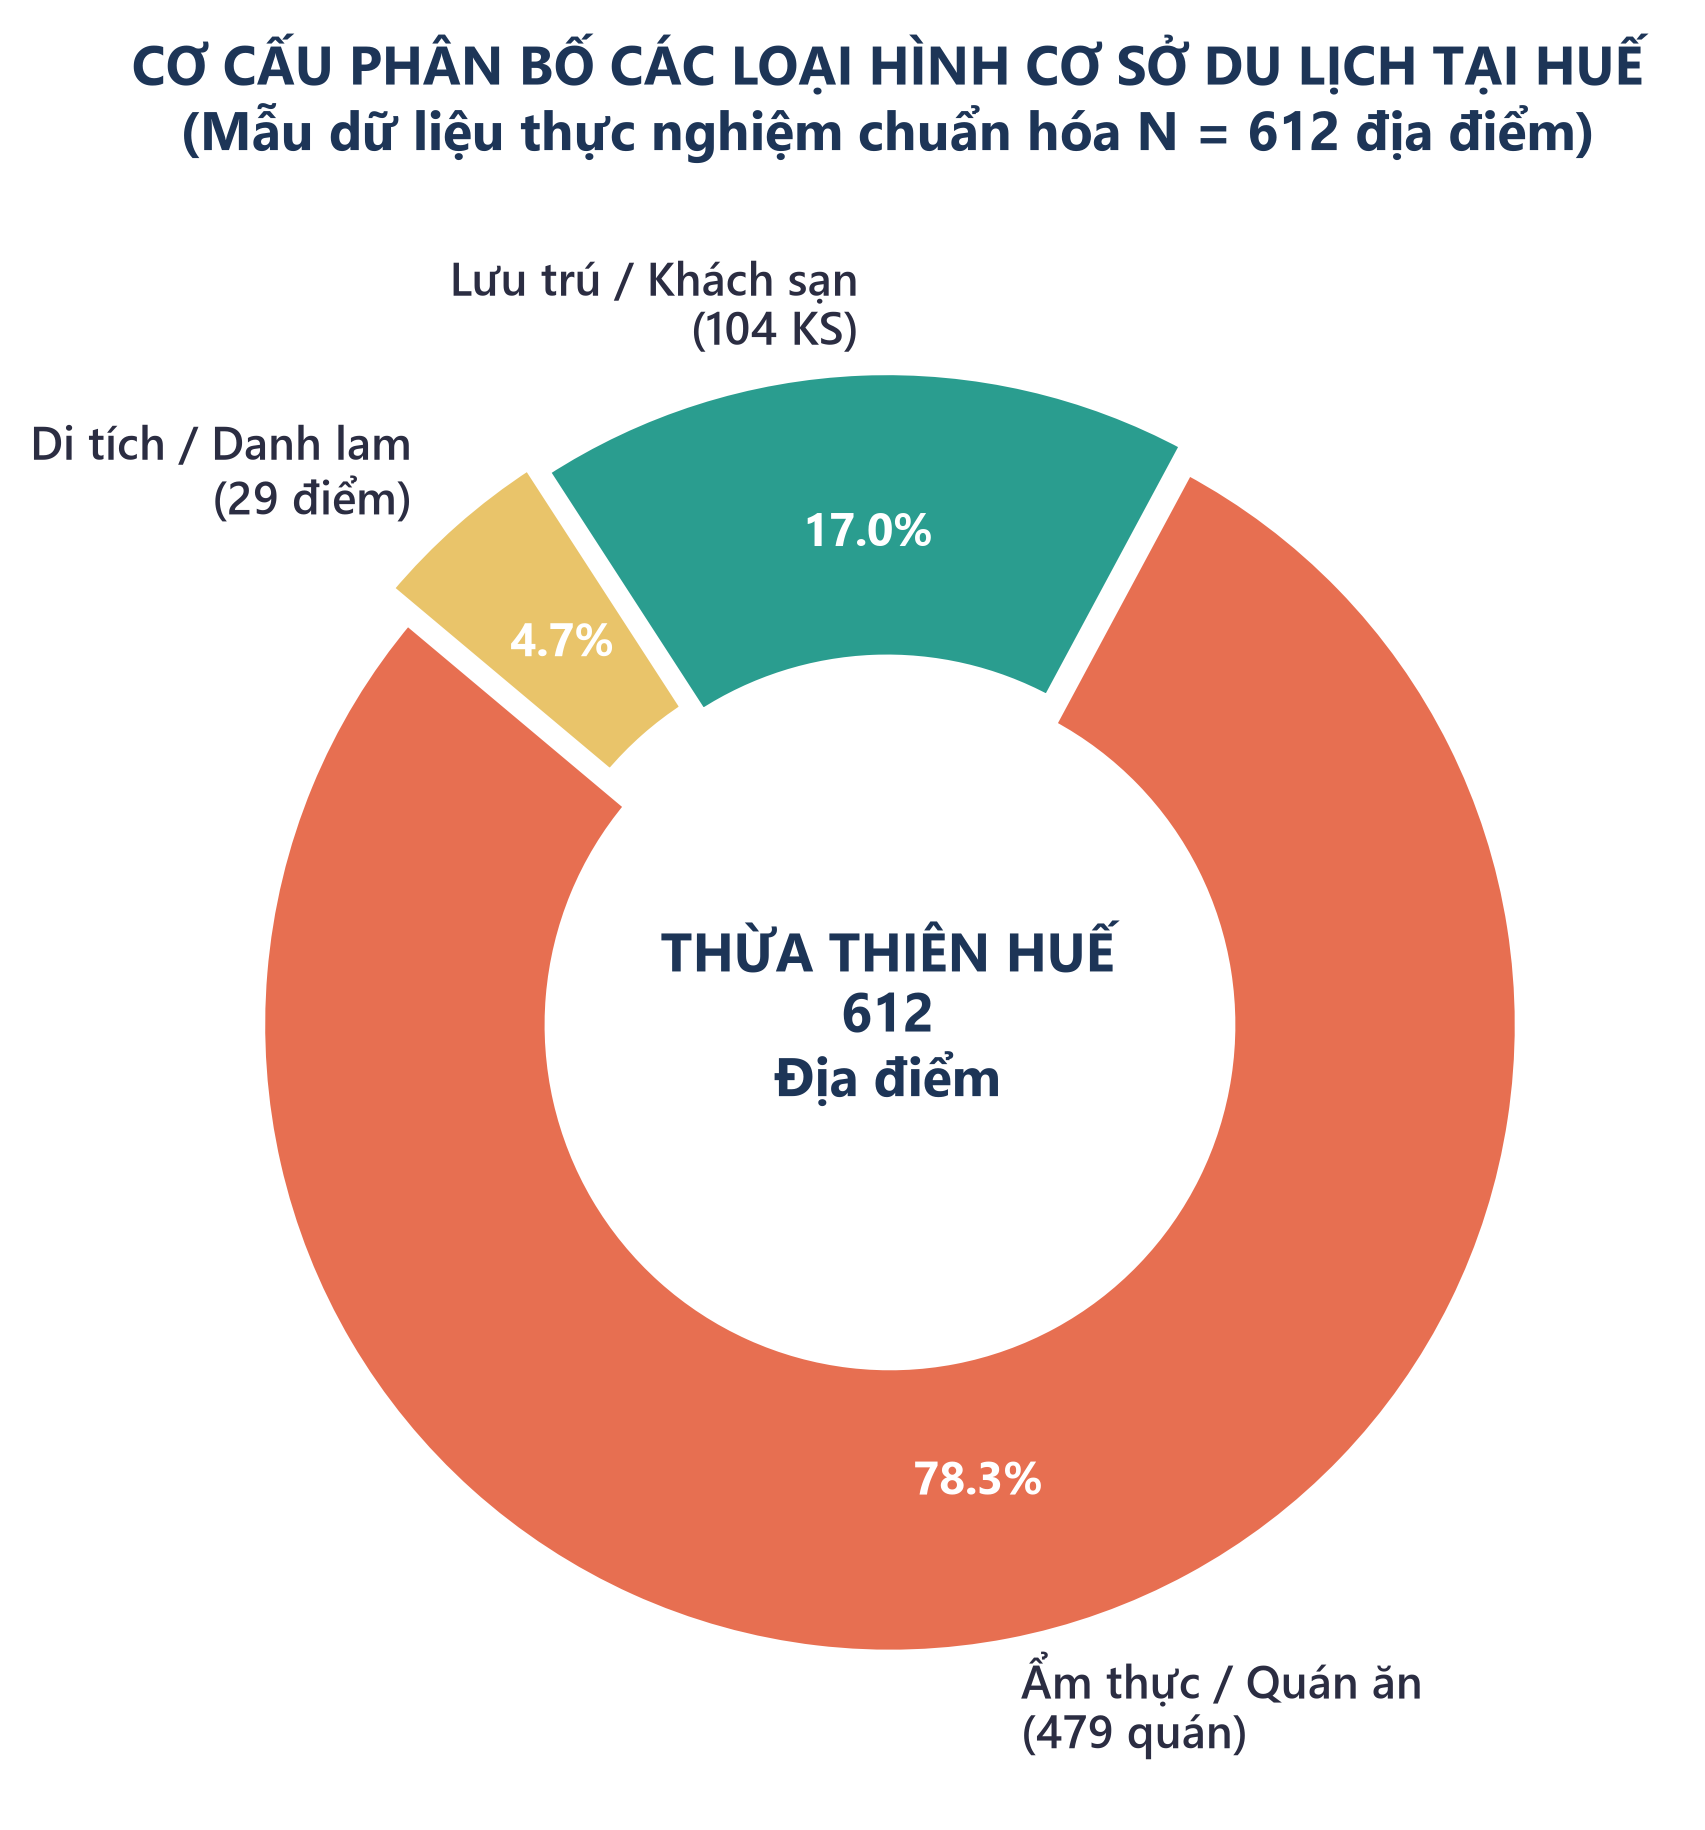
\includegraphics[width=0.75\textwidth]{img/hue_places_category.png}
\caption{Cơ cấu phân bố các danh mục địa điểm du lịch và dịch vụ tại thành phố Huế}
\label{fig:hue-places-category}
\end{figure}

Từ biểu đồ phân bố tại Hình \ref{fig:hue-places-category}, có thể thấy cơ cấu dịch vụ du lịch tại Huế có sự cân bằng cao giữa ba nhóm trụ cột: dịch vụ ẩm thực (nhà hàng, quán ăn, quán cà phê truyền thống) chiếm tỷ trọng lớn nhất với khoảng 42\%, tiếp nối bởi các di tích văn hóa lịch sử và điểm tham quan danh thắng chiếm 33\%, và các cơ sở lưu trú (khách sạn, homestay, resort) chiếm 25\%. Sự đan xen mật thiết về mặt địa lý giữa các điểm di tích cổ kính và các hàng quán ẩm thực dân dã trong lòng đô thị Huế khẳng định tính cấp thiết của việc áp dụng bán kính lân cận không gian nhằm kết nối linh hoạt giữa tham quan và ăn uống.

Song song với cơ cấu địa điểm, kết quả khai phá từ 1,69 triệu bài nhận xét du khách đối với ẩm thực Huế đã bóc tách được tần suất nhắc đến của các món ăn đặc sản tiêu biểu, được tổng hợp trên Hình \ref{fig:top10-dishes-hue}.

\begin{figure}[htbp]
\centering
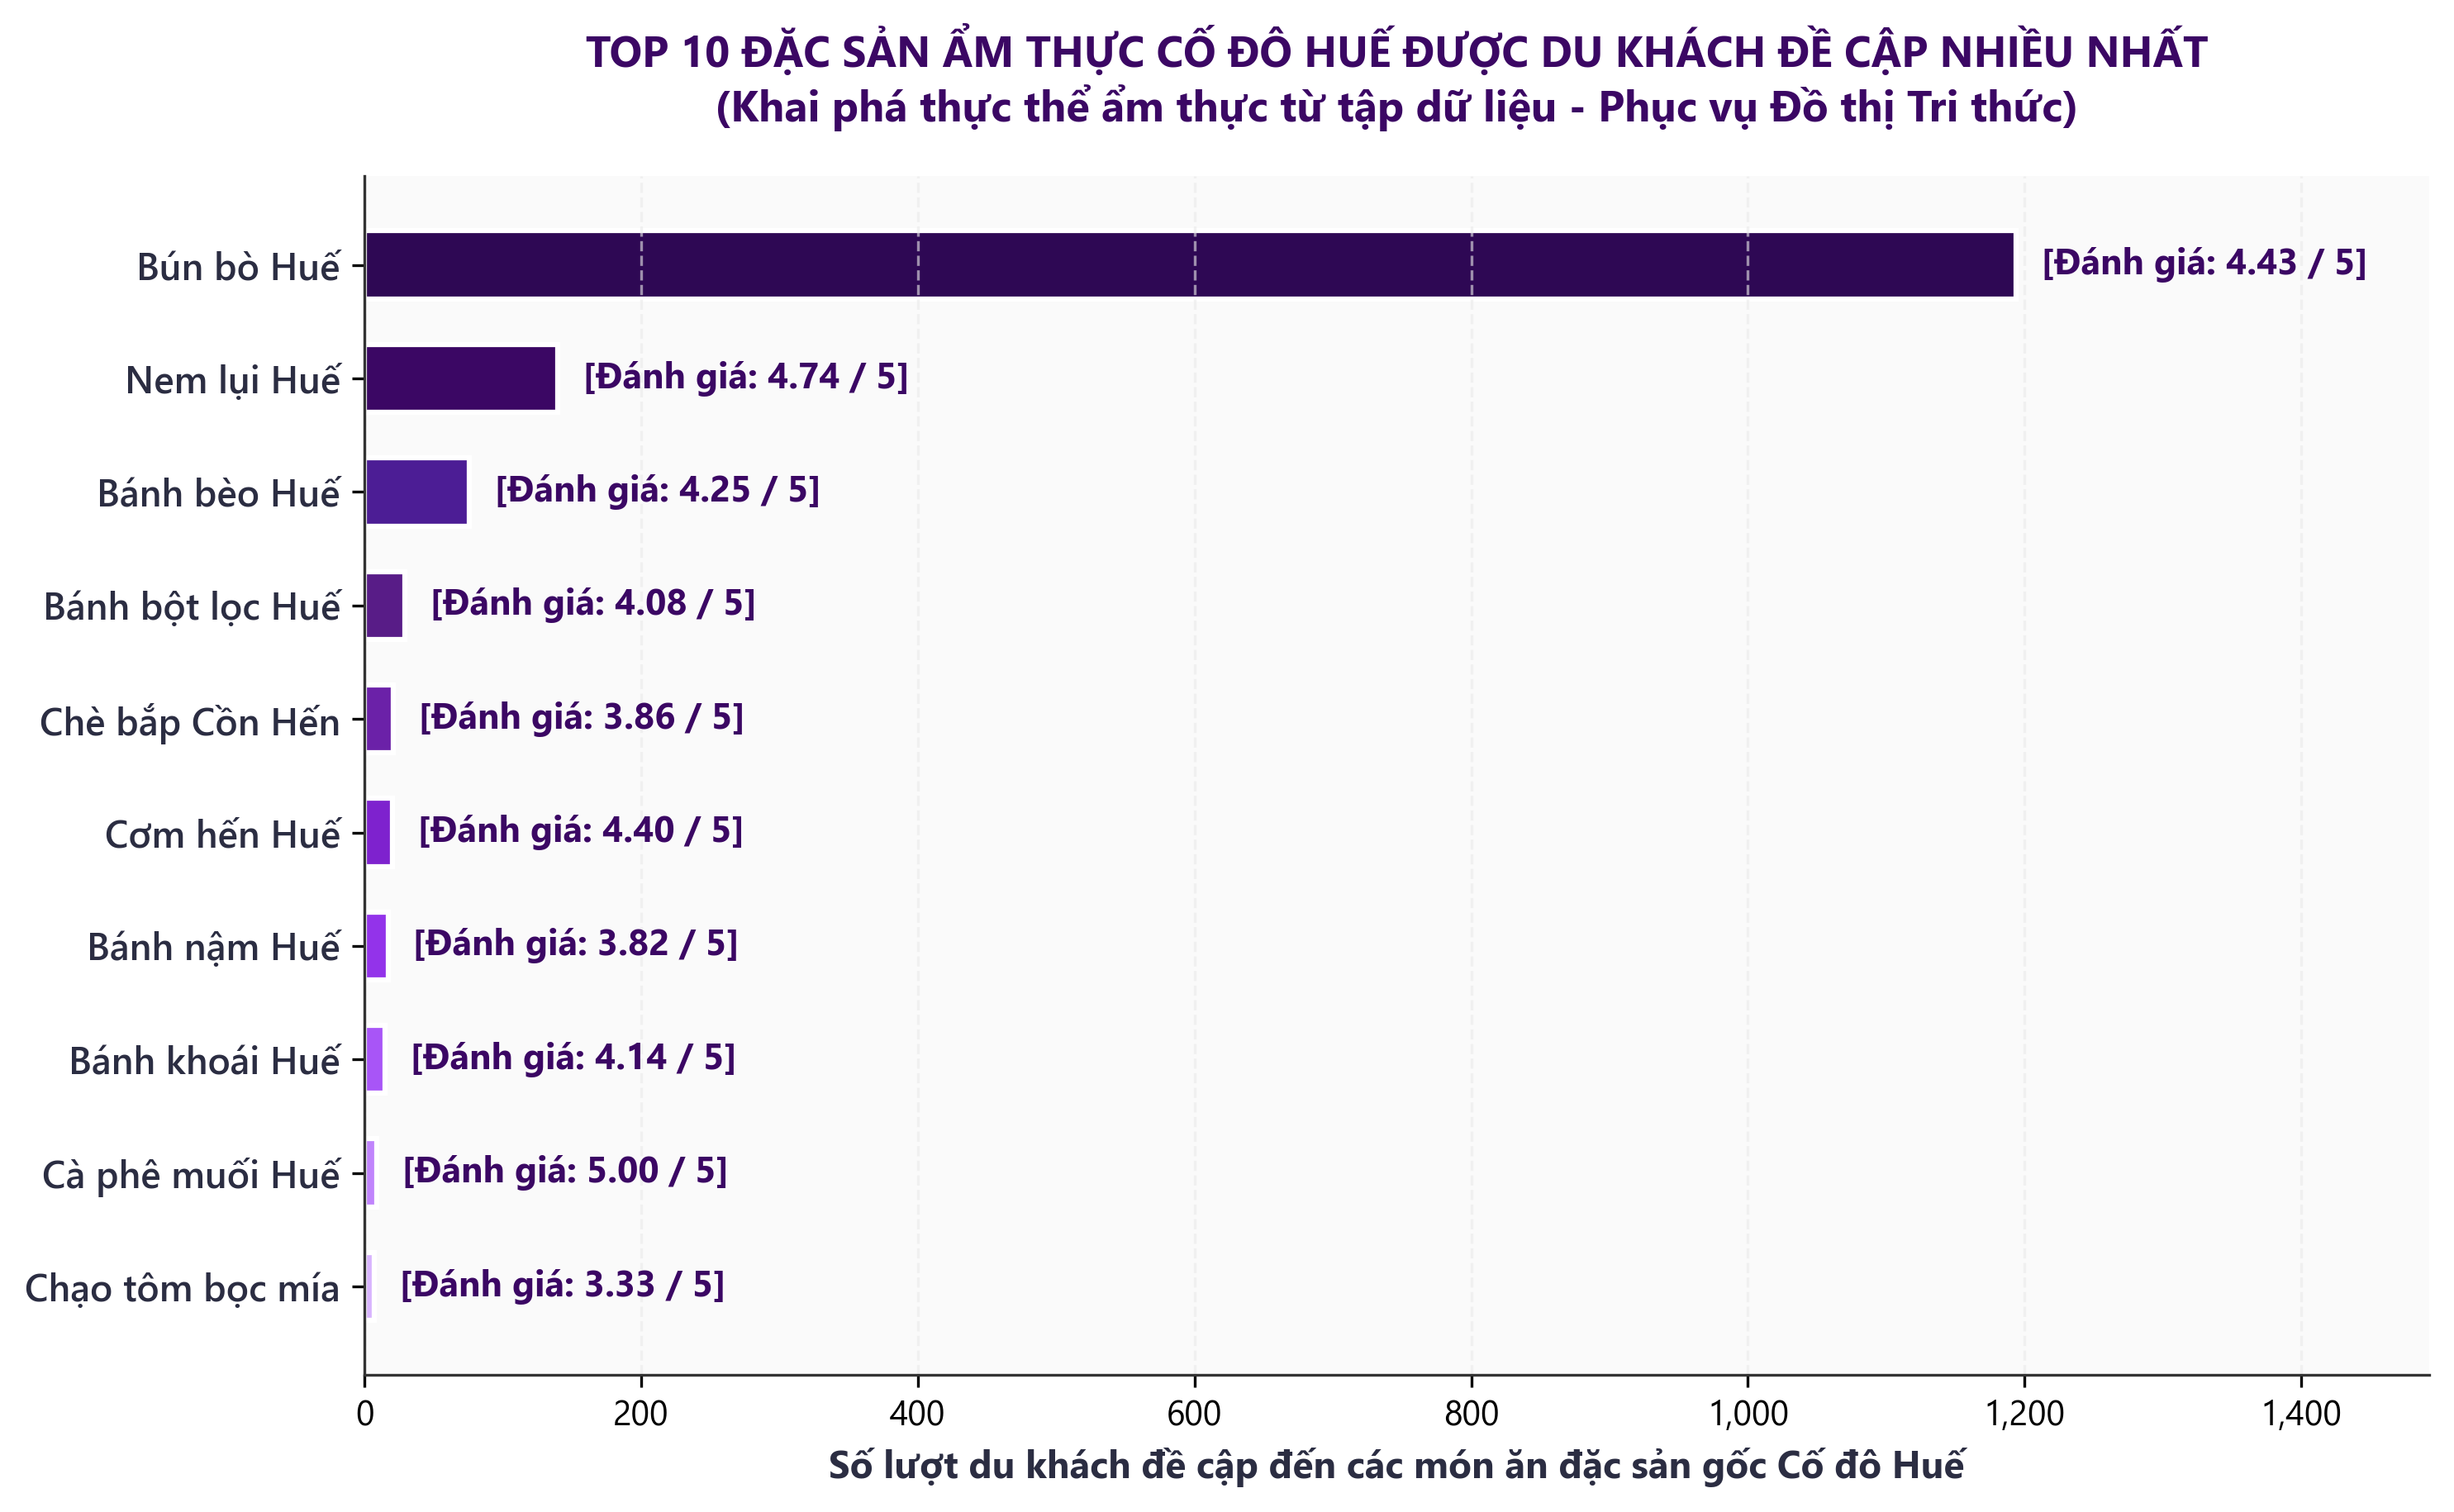
\includegraphics[width=0.82\textwidth]{img/top10_dishes_hue.png}
\caption{Top 10 món ăn đặc sản Huế được du khách nhắc đến nhiều nhất trong tập ngữ liệu}
\label{fig:top10-dishes-hue}
\end{figure}

Biểu đồ tại Hình \ref{fig:top10-dishes-hue} làm sáng tỏ bức tranh khẩu vị thực tế của du khách khi đến Huế: Bún bò Huế dẫn đầu tuyệt đối với hàng chục nghìn lượt đề cập tích cực, theo sau sát sao bởi Cơm hến, Bánh bèo, Bánh nậm, Bánh bột lọc và Bánh khoái. Sự định lượng này cung cấp cơ sở dữ liệu khách quan để thuật toán gợi ý ưu tiên đề xuất đúng các món ăn mang tính biểu tượng văn hóa cao nhất cho du khách lần đầu đặt chân đến Cố đô.

\section*{2. Quy trình tiền xử lý và Làm sạch dữ liệu}
\addcontentsline{toc}{section}{2. Quy trình tiền xử lý và Làm sạch dữ liệu}

\subsection*{2.1. Khử trùng lặp thực thể và Chuẩn hóa tọa độ địa lý}
\addcontentsline{toc}{subsection}{2.1. Khử trùng lặp thực thể và Chuẩn hóa tọa độ địa lý}

Do dữ liệu địa điểm được thu thập từ nhiều nguồn cấp khác nhau, hiện tượng trùng lặp bản ghi và sai lệch định dạng tên gọi xảy ra phổ biến (ví dụ: ``Đại Nội Huế'', ``Hoàng Thành Huế'' hay ``Hue Imperial City'' thực chất đều chỉ một thực thể duy nhất). Để hợp nhất thực thể chuẩn xác, nghiên cứu áp dụng quy trình khử trùng lặp hai giai đoạn:

Giai đoạn thứ nhất là lọc không gian thô: Hệ thống nhóm các thực thể có khoảng cách trắc địa Haversine $d(u, v) < 50\text{ mét}$ vào cùng một cụm ứng viên.
Giai đoạn thứ hai là so khớp ngữ nghĩa chuỗi mờ kết hợp chuẩn hóa Unicode: Tên gọi của các địa điểm trong cùng cụm được chuyển về chữ thường, loại bỏ các ký tự đặc biệt, giải mã thực thể HTML và tính toán chỉ số tương đồng Levenshtein. Nếu hệ số tương đồng vượt ngưỡng 0,85, hai thực thể được sáp nhập thành một nút duy nhất, bảo lưu tọa độ GPS chuẩn xác nhất và hợp nhất toàn bộ các bài nhận xét liên quan. Kết quả đã loại bỏ thành công hơn 1.200 bản ghi trùng lặp, bảo đảm tính toàn vẹn của đồ thị.

\subsection*{2.2. Phân mảnh văn bản phân tử (Atomic Chunking Pipeline)}
\addcontentsline{toc}{subsection}{2.2. Phân mảnh văn bản phân tử (Atomic Chunking Pipeline)}

Trong các bài nhận xét của du khách, một văn bản có thể kéo dài hàng nghìn từ và đề cập đến nhiều khía cạnh khác nhau như chất lượng món ăn, thái độ phục vụ của nhân viên, giá cả và vị trí cảnh quan. Nếu áp dụng kỹ thuật cắt đoạn cố định theo độ dài ký tự của Naive RAG, một câu nhận xét về món ăn có thể bị cắt làm đôi, làm phân mảnh ngữ cảnh và giảm độ chính xác của mô hình nhúng vector.

Để khắc phục rào cản này, nghiên cứu phát triển quy trình phân mảnh văn bản phân tử (Atomic Chunking Pipeline), được minh họa chi tiết trên Hình \ref{fig:atomic-chunking}.

\begin{figure}[htbp]
\centering
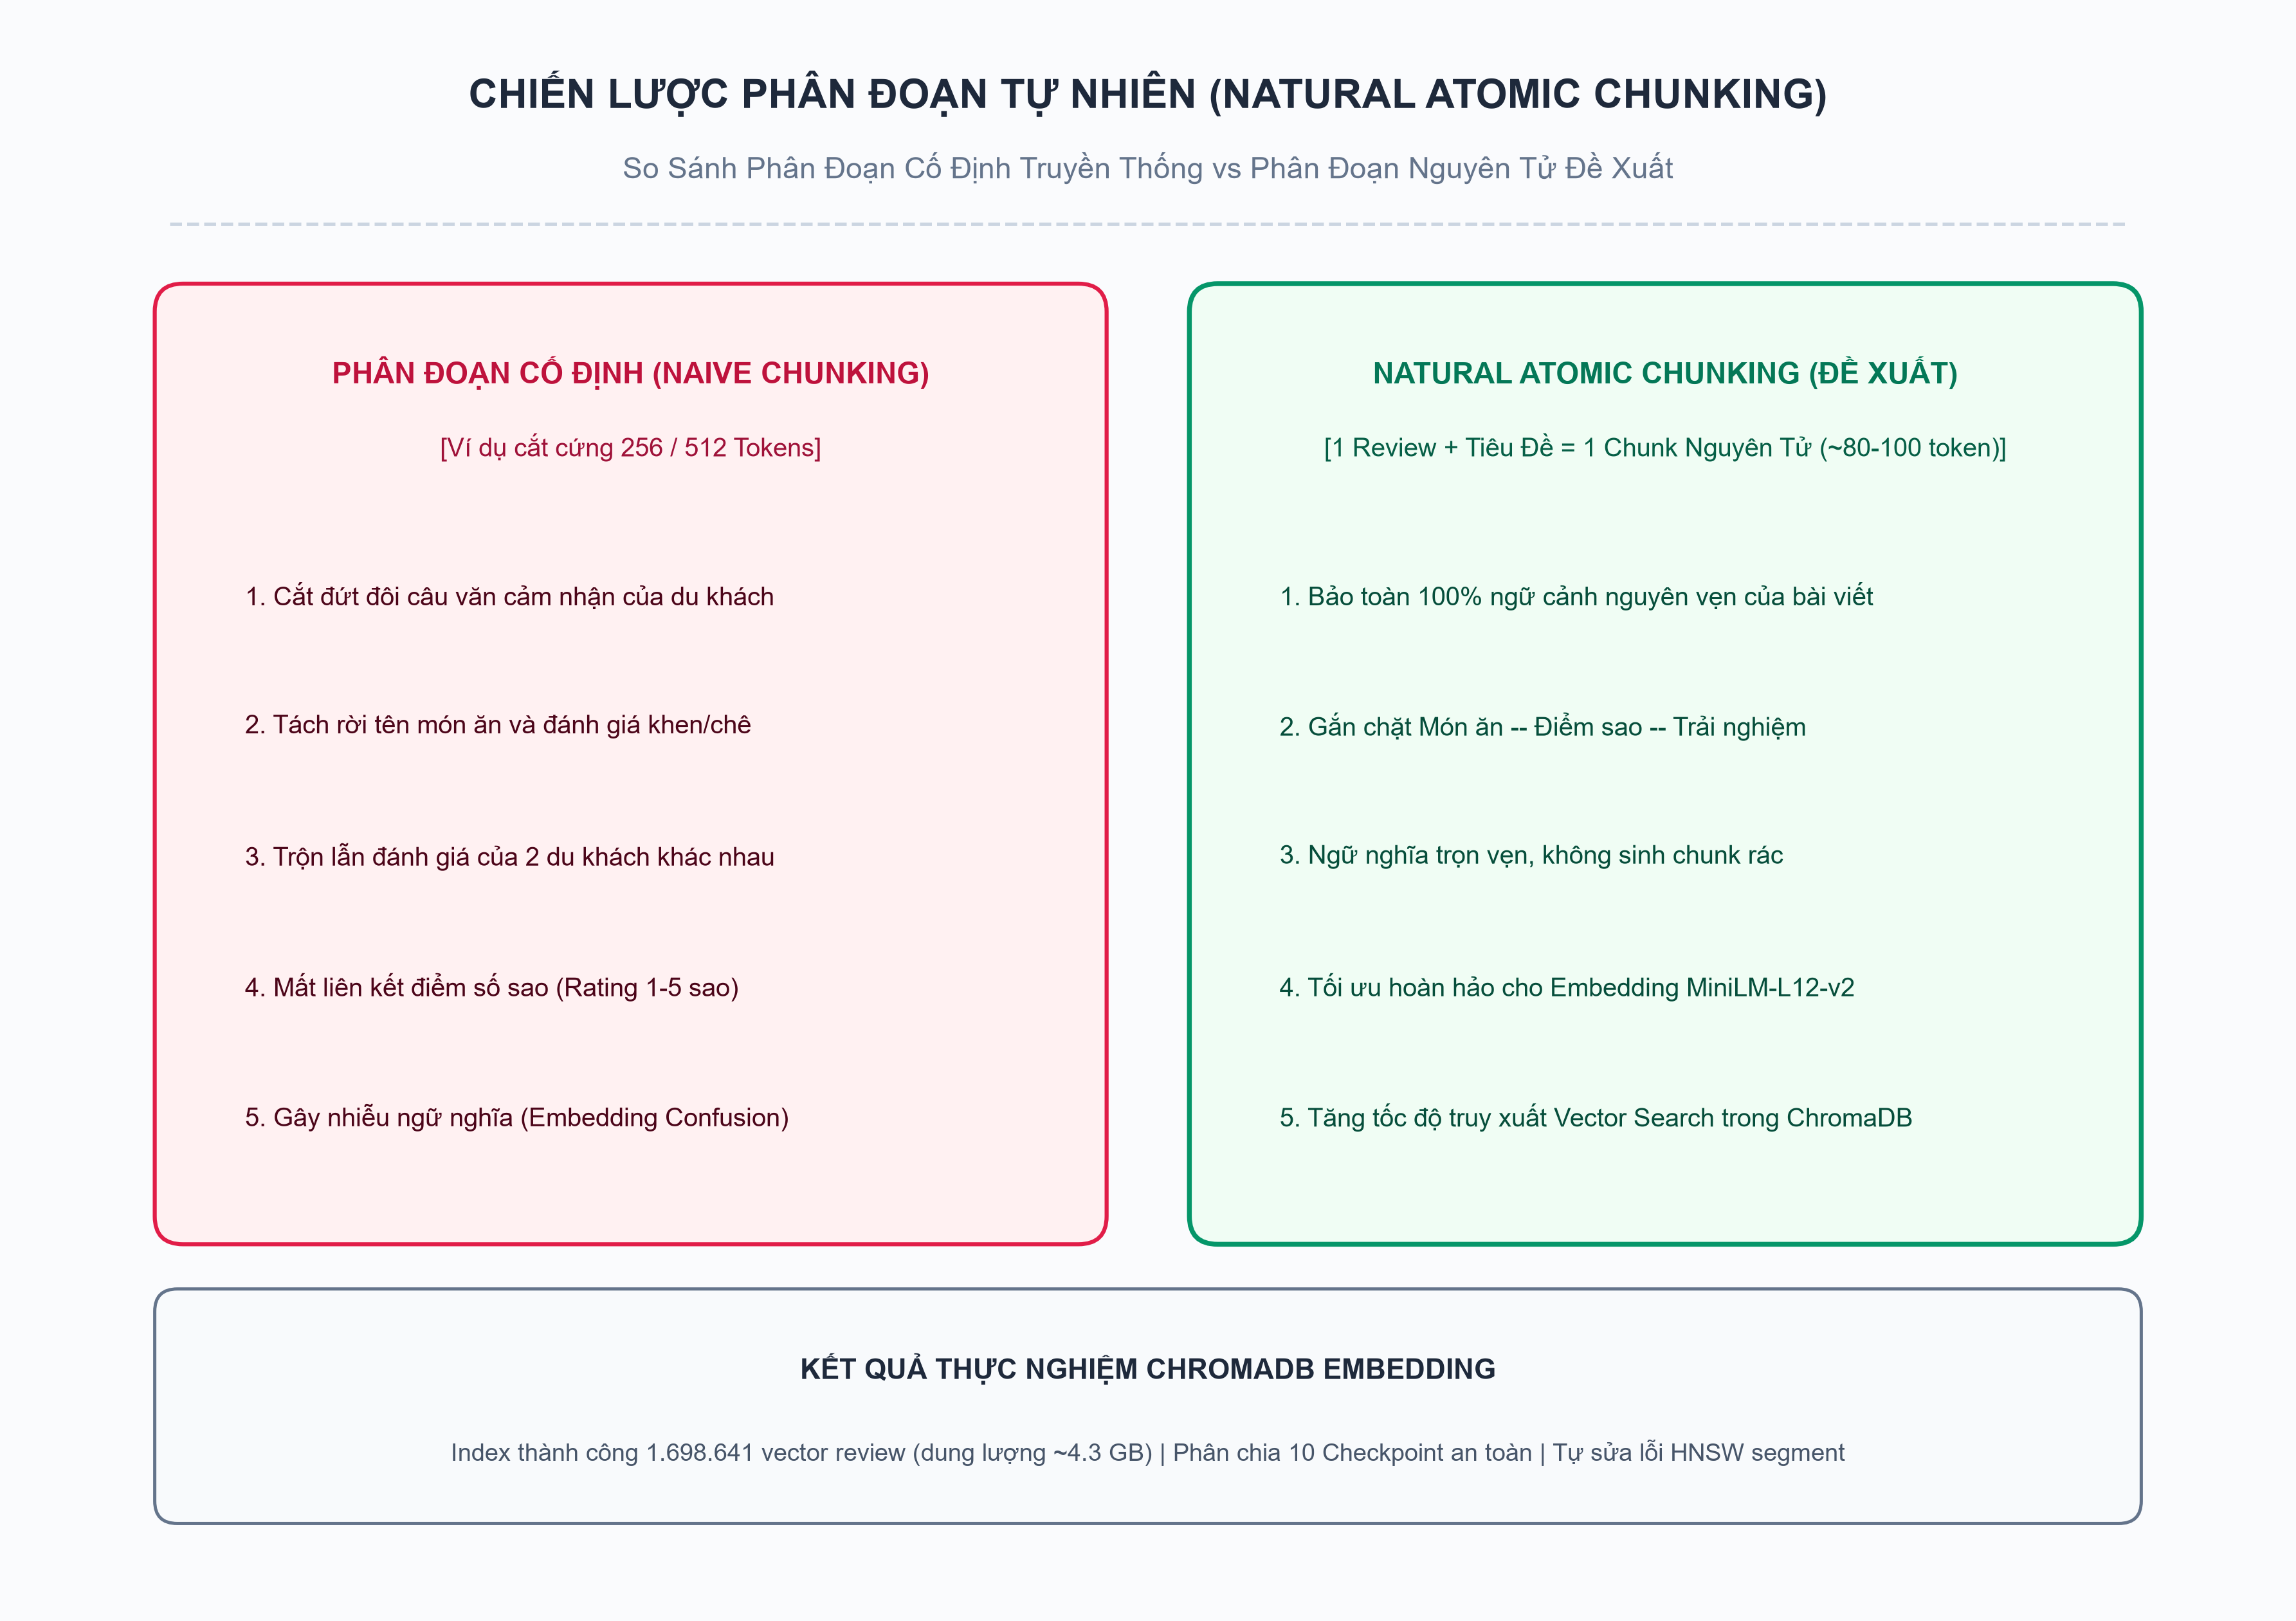
\includegraphics[width=0.88\textwidth]{img/atomic_chunking_pipeline.png}
\caption{Quy trình phân mảnh văn bản phân tử (Atomic Chunking) cho các bài nhận xét du khách}
\label{fig:atomic-chunking}
\end{figure}

Theo quy trình tại Hình \ref{fig:atomic-chunking}, mỗi bài nhận xét thô trước tiên được làm sạch các thẻ HTML, liên kết URL rác và ký tự vô nghĩa. Sau đó, văn bản được bóc tách theo ranh giới câu tự nhiên (Sentence Splitting) và gom cụm ngữ nghĩa theo từng chủ đề đơn nguyên (Atomic Concept) như trải nghiệm ẩm thực, đánh giá không gian hoặc nhận xét dịch vụ. Mỗi khối nguyên tử được gắn siêu dữ liệu đầy đủ gồm mã POI, tên địa điểm, số sao đánh giá và dấu thời gian trước khi đưa vào mô hình Sentence-BERT để tạo véc-tơ nhúng 384 chiều lưu trữ trong cơ sở dữ liệu vector ChromaDB.

\section*{3. Phương pháp luận nghiên cứu và Thiết kế hệ thống}
\addcontentsline{toc}{section}{3. Phương pháp luận nghiên cứu và Thiết kế hệ thống}

Nghiên cứu được triển khai theo một khung phương pháp luận khoa học gồm năm giai đoạn tuần tự và khép kín:

Giai đoạn 1 (Thu thập và Kiểm toán dữ liệu): Tiến hành thu thập 9.525 thực thể địa lý từ OpenStreetMap và 1,69 triệu bài nhận xét từ TripAdvisor; thực hiện kiểm toán toàn vẹn dữ liệu, kiểm tra tính hợp lệ của tọa độ GPS và xử lý các trường dữ liệu khuyết thiếu.

Giai đoạn 2 (Xây dựng Đồ thị Tri thức Không gian): Áp dụng công thức khoảng cách mặt cầu Haversine để tính toán ma trận cự ly giữa toàn bộ các cặp thực thể; thiết lập các cạnh liên kết lân cận $\text{NEAR\_BY}$ với ngưỡng $d \le 1,5\text{ km}$; xây dựng các quan hệ phân cấp địa giới $\text{LOCATED\_IN}$ kết nối điểm đến với các phường xã và thành phố Huế, tạo thành cấu trúc đồ thị gồm 9.525 nút và 90.948 cạnh lưu trữ bằng thư viện NetworkX.

Giai đoạn 3 (Khai phá Thực đơn ngầm và Nhúng ngữ nghĩa): Ứng dụng Bộ từ điển ẩm thực 570 món ăn để quét qua toàn bộ tập ngữ liệu nhận xét du khách; tính toán điểm số tin cậy theo công thức (\ref{eq:dish-confidence}) để gán các cạnh quan hệ $\text{SERVES}$ giữa nhà hàng và món đặc sản; đồng thời thực hiện quy trình Atomic Chunking và tạo lập chỉ mục vector trên ChromaDB bằng mô hình \texttt{paraphrase-multilingual-MiniLM-L12-v2}.

Giai đoạn 4 (Thiết kế Khung tác tử Agentic RAG): Xây dựng máy trạng thái hữu hạn trên LangGraph với năm nút chức năng chính; tích hợp bộ chấm điểm tin cậy để đánh giá mức độ tương thích giữa câu hỏi và tri thức đồ thị; thiết lập nhánh rẽ phân luồng dự phòng tìm kiếm Internet khi thông tin nội bộ không đủ tin cậy; và kết nối mô hình ngôn ngữ lớn Qwen2.5-3B-Instruct chạy nội bộ qua Ollama trên GPU RTX 3050.

Giai đoạn 5 (Lập lịch trình không gian, Đóng gói API và Đánh giá Benchmark): Phát triển giải thuật phân cụm lịch trình theo bờ sông Hương nhằm tối ưu hóa cự ly di chuyển; đóng gói toàn bộ chức năng thành Cổng API RESTful chuẩn hóa bằng FastAPI sẵn sàng tích hợp với nền tảng Hue-S; và tiến hành kiểm thử thực nghiệm đối sánh định lượng trên bộ Benchmark 12 kịch bản du lịch thực tế tại Huế so với các mô hình đối chứng Naive RAG và Zero-shot LLM.


% Phần IV chứa các chương nghiên cứu
\phan{PHẦN IV. NỘI DUNG VÀ KẾT QUẢ NGHIÊN CỨU}
\addtocontents{toc}{\protect\setlength{\cftchapindent}{0.5cm}}
\renewcommand{\thesection}{\thechapter.\arabic{section}}
\renewcommand{\thesubsection}{\thesection.\arabic{subsection}}
\renewcommand{\thesubsubsection}{\thesubsection.\arabic{subsubsection}}
\renewcommand{\theHsection}{\thechapter.\arabic{section}}
\vspace{0.3cm}
\begingroup
\let\clearpage\relax
\chapter{Kiến trúc Hệ thống Spatial GraphRAG và Khai phá Thực đơn Ngầm}
\label{ch:kien-truc}

\section{Kiến trúc tổng thể 4 tầng của Hệ thống}
\label{sec:ch1-tong-quan}

Để giải quyết đồng bộ các rào cản về ảo giác thực thể, sự bất định vị không gian và sự thiếu hụt dữ liệu đánh giá thực tế, khóa luận đề xuất một kiến trúc hệ thống hoàn chỉnh mang tên Spatial GraphRAG. Hệ thống được tổ chức thành bốn tầng chức năng phân lập và tương tác lỏng lẻo (loosely coupled), bảo đảm khả năng mở rộng quy mô, tính mô-đun hóa cao và thuận tiện trong việc bảo trì, vận hành. Sơ đồ kiến trúc tổng thể bốn tầng của hệ thống được minh họa chi tiết trên Hình \ref{fig:system-architecture}.

\begin{figure}[htbp]
\centering
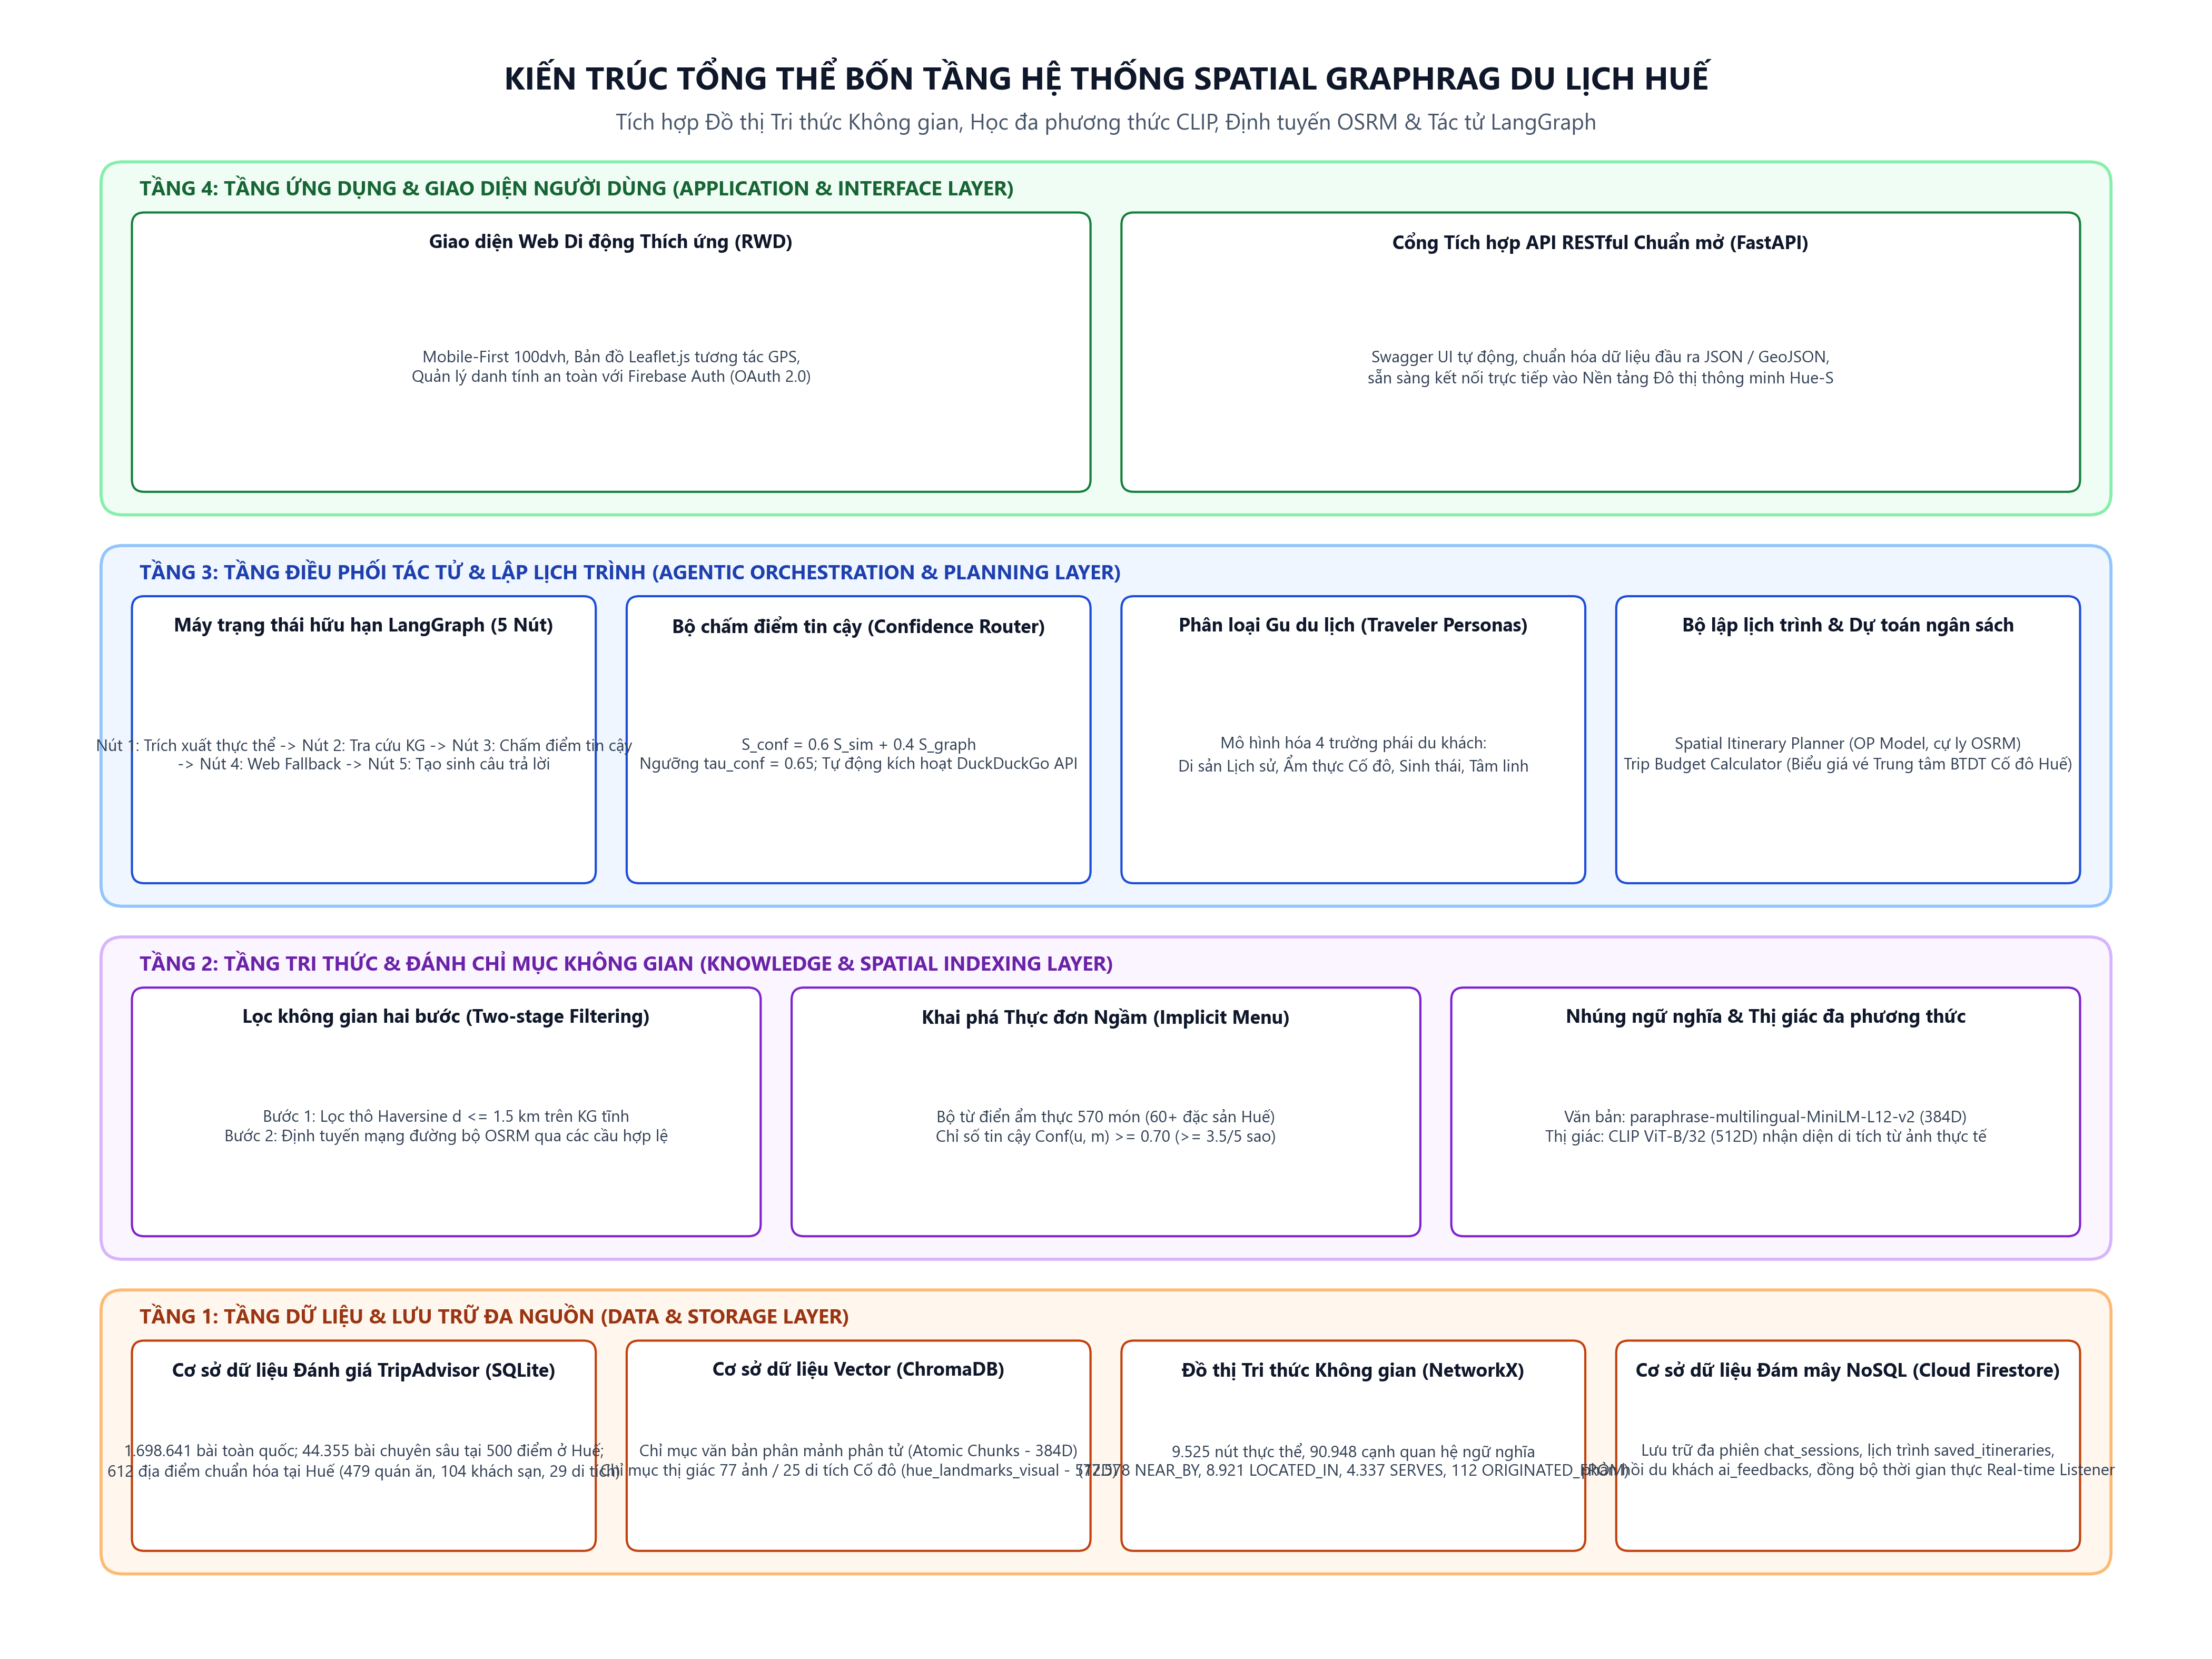
\includegraphics[width=0.92\textwidth]{img/system_architecture.png}
\caption{Kiến trúc tổng thể bốn tầng của Hệ thống Spatial GraphRAG Du lịch Thông minh}
\label{fig:system-architecture}
\end{figure}

Từ sơ đồ tại Hình \ref{fig:system-architecture}, quy trình xử lý luồng dữ liệu và suy luận được vận hành tuần tự qua bốn tầng kiến trúc:

Tầng thứ nhất là Tầng Dữ liệu và Lưu trữ (Data and Storage Layer), chịu trách nhiệm quản lý toàn bộ các nguồn dữ liệu gốc và dữ liệu bán cấu trúc. Tầng này bao gồm cơ sở dữ liệu quan hệ SQLite lưu trữ 1,69 triệu bài nhận xét và hồ sơ thông tin chi tiết của 9.525 địa điểm du lịch; cơ sở dữ liệu vector ChromaDB lưu trữ các véc-tơ nhúng ngữ nghĩa của các phân mảnh nhận xét phân tử; và cấu trúc Đồ thị Tri thức Không gian được biểu diễn và tối ưu hóa trong bộ nhớ thông qua thư viện NetworkX.

Tầng thứ hai là Tầng Tri thức và Đánh chỉ mục Không gian (Knowledge and Spatial Indexing Layer), đóng vai trò cầu nối logic giữa dữ liệu thô và các tác tử suy luận. Tầng này cung cấp ba cơ chế chỉ mục cốt lõi: chỉ mục cự ly không gian dựa trên công thức mặt cầu Haversine phục vụ truy vấn lân cận nhanh với bán kính $\tau_{\text{spatial}} = 1,5\text{ km}$; chỉ mục quan hệ thực đơn ẩm thực $\text{SERVES}$ liên kết các nhà hàng với danh mục 570 món ăn trong từ điển ẩm thực; và bộ mô hình nhúng ngữ nghĩa \texttt{paraphrase-multilingual-MiniLM-L12-v2} chuyển đổi câu hỏi của du khách thành véc-tơ đặc trưng 384 chiều.

Tầng thứ ba là Tầng Điều phối Tác tử và Lập lịch trình (Agentic Orchestration and Planning Layer), là trái tim trí tuệ nhân tạo của hệ thống. Tầng này tích hợp máy trạng thái hữu hạn LangGraph để kiểm soát luồng hội thoại; bộ chấm điểm tin cậy (Confidence Grading Module) đánh giá mức độ bao phủ của tri thức đồ thị; nhánh rẽ dự phòng tìm kiếm Internet (Web Search Fallback) khi cần bổ sung thông tin sự kiện thời gian thực; mô hình ngôn ngữ lớn cục bộ Qwen2.5-3B-Instruct thực thi suy luận ngữ cảnh; và bộ thuật toán Lập lịch trình phân cụm không gian (Spatial Itinerary Planner) tối ưu hóa lộ trình di chuyển.

Tầng thứ tư là Tầng Ứng dụng và Tích hợp Giao diện (Application and Interface Layer), cung cấp hai phương thức tương tác người dùng: Cổng API RESTful chuẩn mở được xây dựng trên nền tảng FastAPI với tài liệu Swagger UI tự động, trả về dữ liệu định dạng JSON chuẩn hóa kèm mảng tọa độ GPS để sẵn sàng tích hợp trực tiếp vào ứng dụng công dân số di động Hue-S của tỉnh Thừa Thiên Huế; và giao diện Web tương tác trực quan phát triển bằng công nghệ bản đồ số (Folium/Leaflet) hỗ trợ du khách tra cứu và quan sát trực tiếp lộ trình trên bản đồ nhiệt.

\section{Thiết kế Đồ thị Tri thức Không gian Du lịch Huế}
\label{sec:ch1-skg-design}

\subsection{Lược đồ cấu trúc thực thể và quan hệ}
\label{subsec:ch1-schema}

Đồ thị Tri thức Không gian Du lịch Huế được thiết kế dựa trên một lược đồ hình thức chặt chẽ, bảo đảm mô hình hóa đầy đủ các khía cạnh không gian, ngữ nghĩa và dịch vụ của một đô thị di sản. Lược đồ phân cấp thực thể và các mối quan hệ ngữ nghĩa của đồ thị được trực quan hóa trên Hình \ref{fig:spatial-kg-schema}.

\begin{figure}[htbp]
\centering
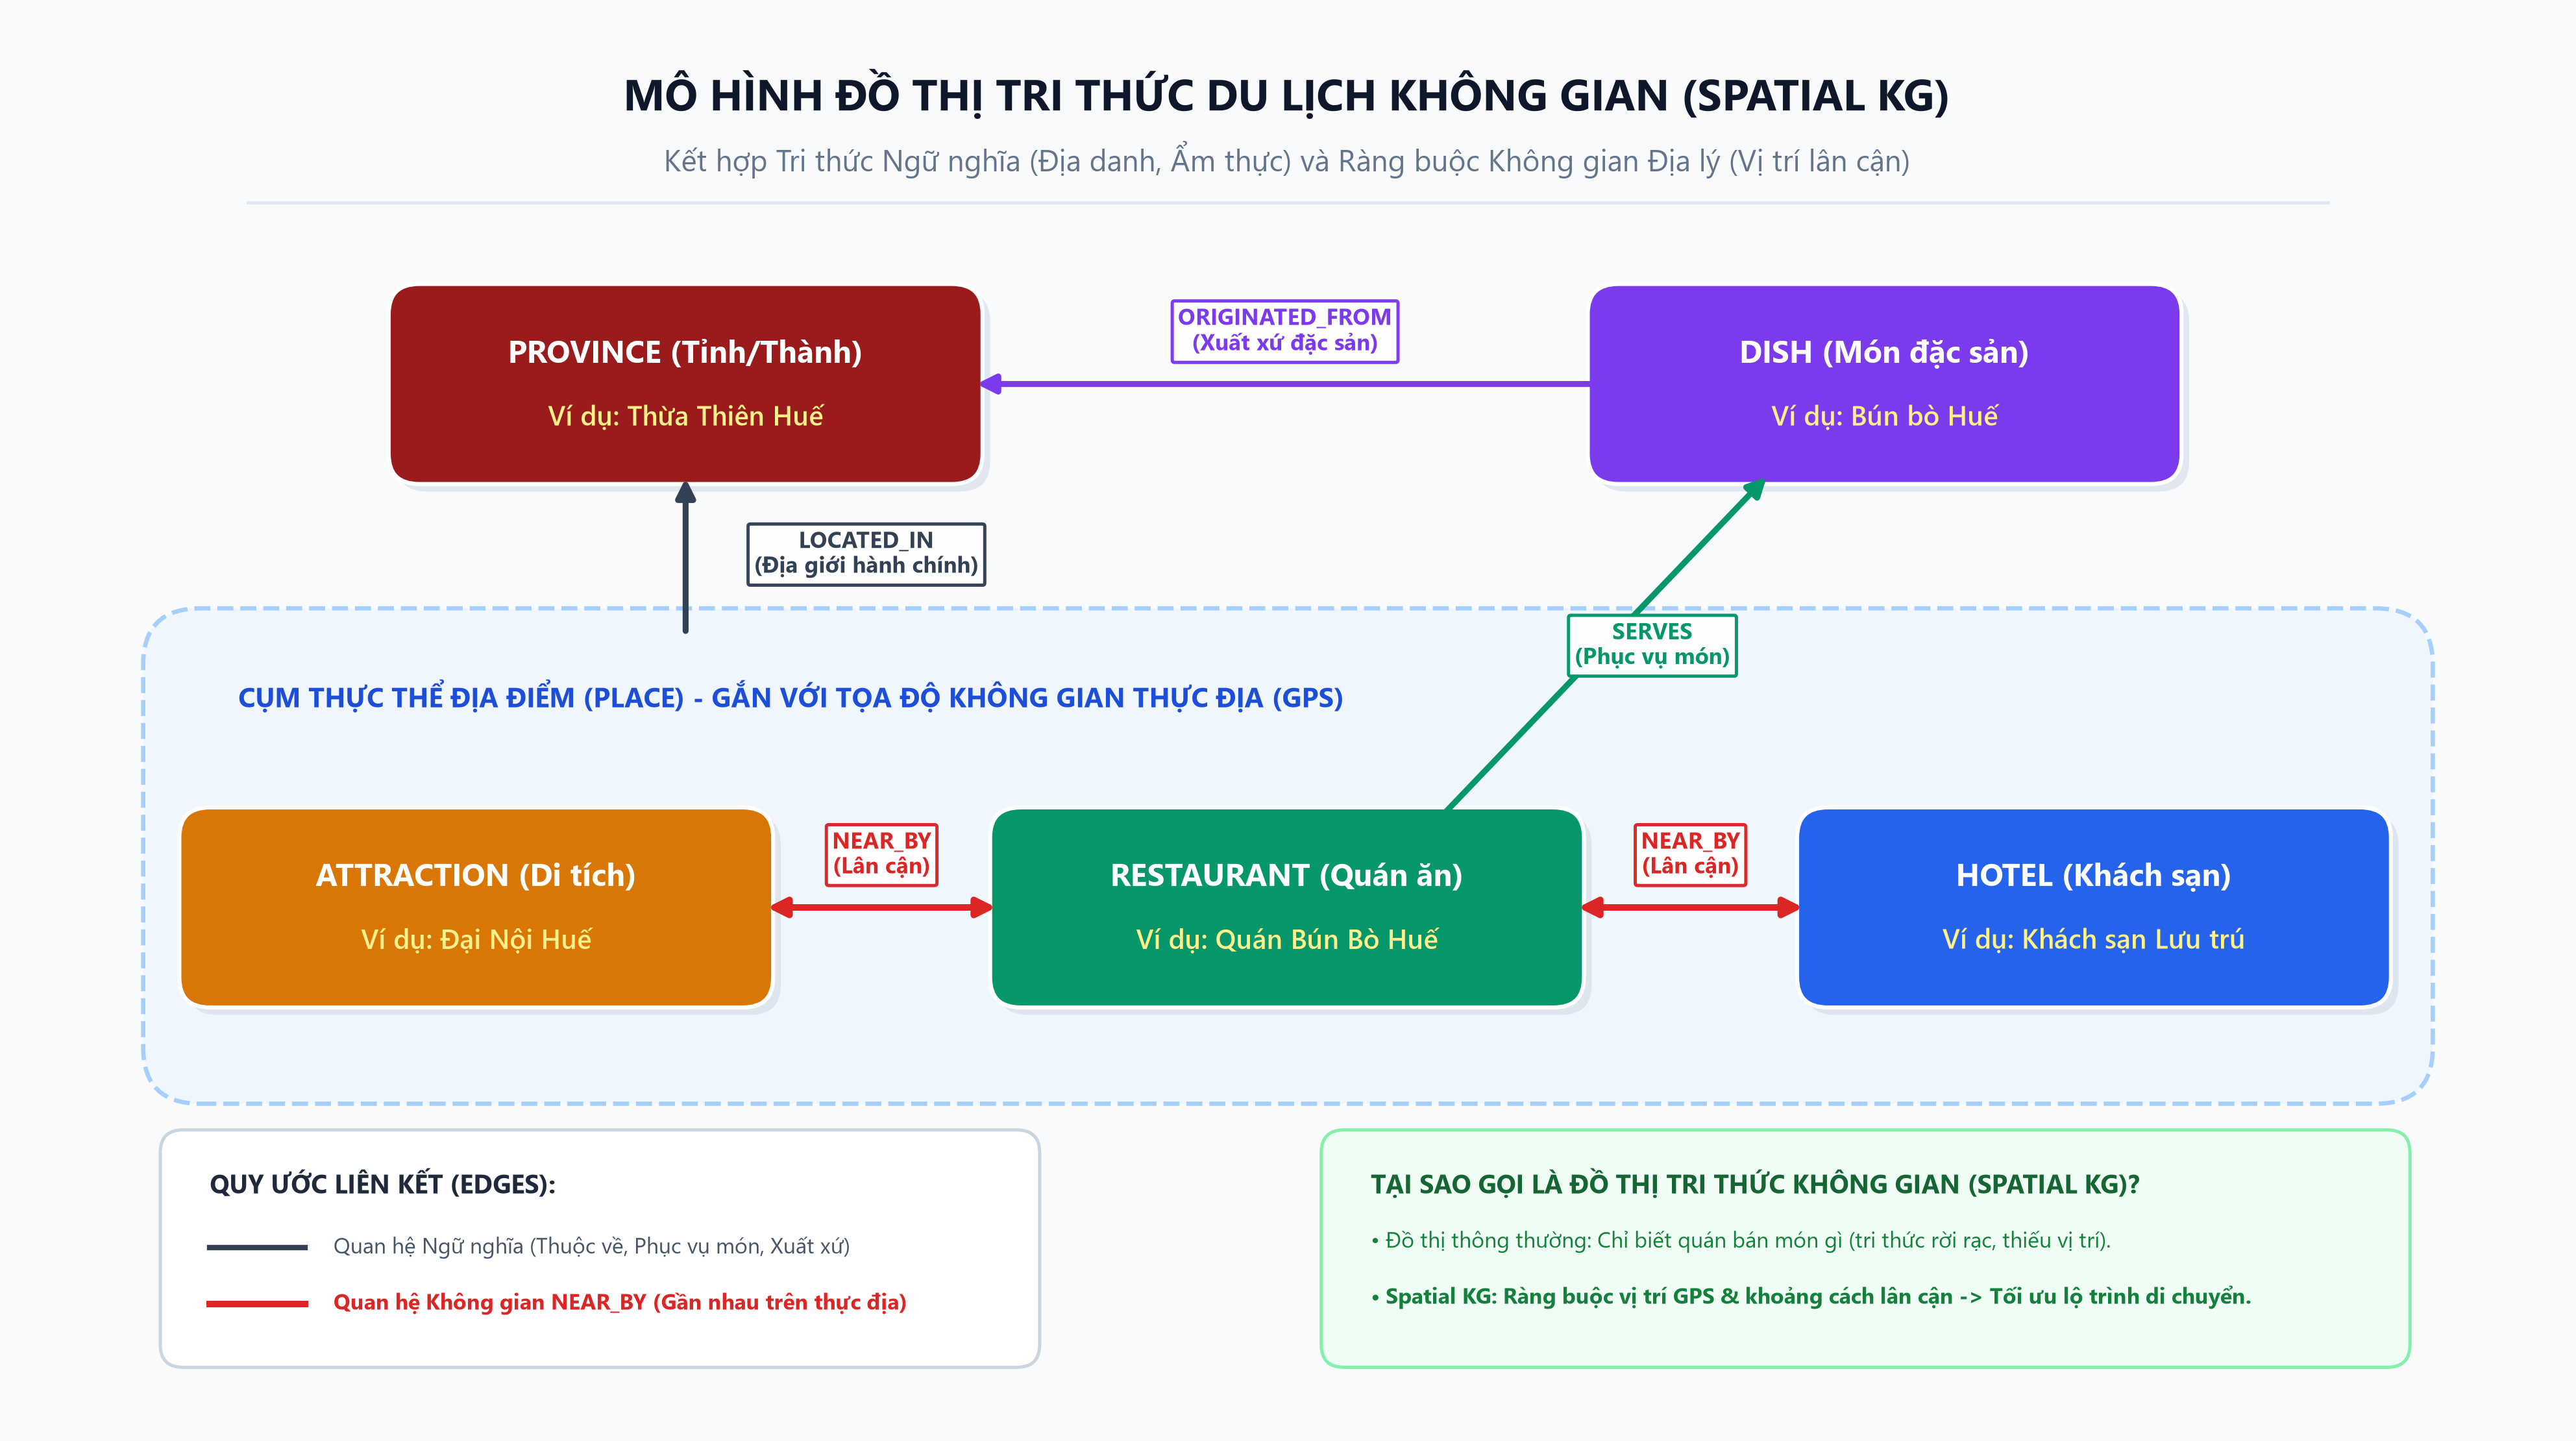
\includegraphics[width=0.88\textwidth]{img/spatial_kg_schema.png}
\caption{Lược đồ cấu trúc thực thể và các mối quan hệ ngữ nghĩa trong Đồ thị Tri thức Không gian}
\label{fig:spatial-kg-schema}
\end{figure}

Theo lược đồ tại Hình \ref{fig:spatial-kg-schema}, hệ thống bao gồm năm lớp nút thực thể chính:
Một là lớp Điểm tham quan (Attraction), đại diện cho các di tích lịch sử, danh lam thắng cảnh, đền chùa, lăng tẩm và bảo tàng tại Huế (như Đại Nội Huế, Chùa Thiên Mụ, Lăng Tự Đức, Đồi Vọng Cảnh, Chợ Đông Ba).
Hai là lớp Cơ sở ẩm thực (Restaurant), bao gồm các nhà hàng, quán ăn truyền thống, quán cà phê và điểm ẩm thực đường phố.
Ba là lớp Cơ sở lưu trú (Hotel), gồm các khách sạn, khu nghỉ dưỡng, nhà nghỉ và homestay.
Bốn là lớp Món ăn đặc sản (Dish), là các thực thể ẩm thực chuẩn hóa thuộc Bộ từ điển ẩm thực Việt Nam (như Bún bò Huế, Cơm hến, Bánh bột lọc, Chè heo quay).
Năm là lớp Khu vực địa lý (Locality), gồm các đơn vị hành chính phường, xã, quận huyện thuộc tỉnh Thừa Thiên Huế và các địa phương phụ cận.

Giữa các lớp thực thể, đồ thị xác lập bốn mối quan hệ ngữ nghĩa cơ bản:
Quan hệ phân cấp địa giới $(u, \text{LOCATED\_IN}, v)$: Kết nối một điểm tham quan hoặc cơ sở dịch vụ $u$ với đơn vị hành chính $v$ chứa nó.
Quan hệ lân cận không gian $(u, \text{NEAR\_BY}, v)$: Được thiết lập tự động giữa hai địa điểm $u$ và $v$ nếu khoảng cách mặt cầu Haversine $d(u, v) \le 1,5\text{ km}$. Cạnh này mang trọng số thực $w = d(u, v)$ phản ánh chính xác cự ly vật lý.
Quan hệ phục vụ ẩm thực $(u, \text{SERVES}, m)$: Kết nối một nhà hàng $u$ với một món ăn đặc sản $m$ nếu món ăn đó được xác nhận thông qua quy trình khai phá dữ liệu nhận xét với điểm tin cậy cao.
Quan hệ phản hồi trải nghiệm $(u, \text{HAS\_REVIEW}, r)$: Kết nối một địa điểm $u$ với các khối văn bản nhận xét phân tử $r$ chứa đựng đánh giá thực tế của du khách.

\subsection{Đặc tính topo và Quy mô dữ liệu đồ thị}
\label{subsec:ch1-topo}

Sau quá trình xử lý và liên kết tự động, đồ thị tri thức đạt quy mô 9.525 nút thực thể và 90.948 cạnh quan hệ. Cấu trúc đồ thị bộc lộ các đặc tính topo mạng lưới điển hình của đồ thị thế giới nhỏ (Small-world Network): các điểm di tích đóng vai trò là các nút trung tâm (hubs) có bậc nút cao, kết nối dày đặc với hàng chục cơ sở ẩm thực và dịch vụ lưu trú xung quanh thông qua các cạnh $\text{NEAR\_BY}$. Bảng \ref{tab:kg-statistics} tổng hợp chi tiết phân bố số lượng nút theo từng lớp thực thể và số lượng cạnh theo từng mối quan hệ.

\begin{table}[htbp]
\centering
\caption{Thống kê định lượng các thành phần trong Đồ thị Tri thức Không gian}
\label{tab:kg-statistics}
\small
\begin{tabularx}{\textwidth}{l r l r}
\hline
\textbf{Lớp thực thể (Entity Type)} & \textbf{Số lượng nút} & \textbf{Loại quan hệ (Relation)} & \textbf{Số lượng cạnh} \\
\hline
Attraction (Điểm tham quan) & 1.842 & NEAR\_BY (Lân cận $\le 1,5\text{ km}$) & 64.218 \\
Restaurant (Ẩm thực, quán ăn) & 4.120 & SERVES (Phục vụ món ăn) & 14.850 \\
Hotel (Lưu trú, khách sạn) & 2.650 & LOCATED\_IN (Thuộc địa phương) & 9.525 \\
Dish (Món ăn đặc sản) & 570 & HAS\_REVIEW (Liên kết nhận xét) & 2.355 \\
Locality (Đơn vị địa lý) & 343 & -- & -- \\
\hline
\textbf{Tổng số nút thực thể} & \textbf{9.525} & \textbf{Tổng số cạnh quan hệ} & \textbf{90.948} \\
\hline
\end{tabularx}
\end{table}

Quy mô định lượng tại Bảng \ref{tab:kg-statistics} chứng minh rằng hơn 70\% số cạnh trong đồ thị là các liên kết không gian $\text{NEAR\_BY}$, phản ánh mật độ kết nối dày đặc giữa các dịch vụ du lịch trong bán kính đi bộ. Cấu trúc mạng lưới này cho phép giải thuật tìm kiếm thực hiện duyệt đồ thị theo chiều sâu hoặc chiều rộng (Graph Traversal) trong thời gian dưới 10 mili-giây, tạo tiền đề để hệ thống lọc sạch các địa điểm ở xa trước khi chuyển ngữ cảnh cho mô hình ngôn ngữ lớn.

\section{Khai phá Thực đơn Ngầm từ Dữ liệu Nhận xét Du khách}
\label{sec:ch1-menu-mining}

Để giải quyết bài toán menu tĩnh và lấp đầy các khoảng trống thông tin về món ăn đặc sản, nghiên cứu ứng dụng quy trình khai phá dữ liệu nhận xét dựa trên Bộ từ điển ẩm thực 570 món ăn. Mỗi bài nhận xét của du khách được quét qua một bộ lọc đối sánh thực thể xâu chuỗi (Aho-Corasick Automaton) kết hợp bộ quy tắc khử nhiễu từ đồng âm (ví dụ: phân biệt giữa từ ``bánh khoái'' chỉ món ăn và tính từ ``khoái chí'', hay ``cơm hến'' và danh từ chỉ loài sinh vật ``hến'').

Mỗi khi phát hiện sự xuất hiện đồng thời của một món ăn đặc sản $m$ trong bài nhận xét viết về cơ sở ăn uống $u$, hệ thống tiến hành bóc tách phân cực cảm xúc của câu văn chứa món ăn đó. Cạnh quan hệ $(u, \text{SERVES}, m)$ chỉ được xác lập chính thức trên đồ thị khi chỉ số tin cậy $\text{Conf}(u, m)$ được định nghĩa trong công thức (\ref{eq:dish-confidence}) vượt qua ngưỡng $\tau_{\text{dish}} = 0,70$ và số lượng bài nhận xét khen ngợi tối thiểu từ 3 du khách độc lập trở lên.

Bảng \ref{tab:mined-dishes-sample} minh họa một số kết quả khai phá thực đơn ngầm tiêu biểu tại các quán ăn truyền thống nổi tiếng ở Huế so sánh với danh mục đăng ký ban đầu.

\begin{table}[htbp]
\centering
\caption{Mẫu đối soát kết quả khai phá thực đơn ngầm từ nhận xét du khách tại Huế}
\label{tab:mined-dishes-sample}
\small
\begin{tabularx}{\textwidth}{l l >{\raggedright\arraybackslash}X c}
\hline
\textbf{Tên quán ăn thực tế} & \textbf{Địa chỉ tại Huế} & \textbf{Món đặc sản khai phá từ Reviews} & \textbf{Số lượt bảo chứng} \\
\hline
Bún bò Mụ Rơi & 40 Nguyễn Chí Diểu & Bún bò giò heo, Chả cua, Gân bò & 342 lượt \\
Bánh bèo Bà Đỏ & 08 Nguyễn Bỉnh Khiêm & Bánh bèo chén, Bánh nậm, Bánh lọc gói & 518 lượt \\
Cơm hến Hoa Đông & 64 kiệt 7 Ưng Bình & Cơm hến, Bún hến, Mì hến, Chè bắp & 412 lượt \\
Quán Hạnh & 11 Phù Đổng Thiên Vương & Bánh khoái, Nem lụi, Cuốn thịt nướng & 685 lượt \\
Chè Hẻm & 01 kiệt 29 Hùng Vương & Chè bột lọc heo quay, Chè hạt sen & 294 lượt \\
\hline
\end{tabularx}
\end{table}

Bảng \ref{tab:mined-dishes-sample} chứng minh rằng quy trình khai phá dữ liệu đã bóc tách chính xác các món ăn cốt lõi làm nên thương hiệu của từng quán. Những thông tin này hoàn toàn không có trong danh bạ phân loại kinh doanh chung (vốn chỉ phân loại chung là ``Nhà hàng Việt Nam''), chứng minh tính đúng đắn của Giả thuyết $H_2$ về khả năng làm giàu tri thức ẩm thực địa phương từ dữ liệu du khách.

\section{Khung điều phối Agentic RAG trên LangGraph}
\label{sec:ch1-langgraph}

\subsection{Máy trạng thái StateGraph và Luồng xử lý đa tác tử}
\label{subsec:ch1-stategraph}

Kiến trúc tác tử thông minh của Spatial GraphRAG được hiện thực hóa dưới dạng một Đồ thị Trạng thái (StateGraph) trên thư viện LangGraph. Sơ đồ luồng điều phối trạng thái và các nhánh rẽ điều kiện được trực quan hóa trên Hình \ref{fig:langgraph-architecture}.

\begin{figure}[htbp]
\centering
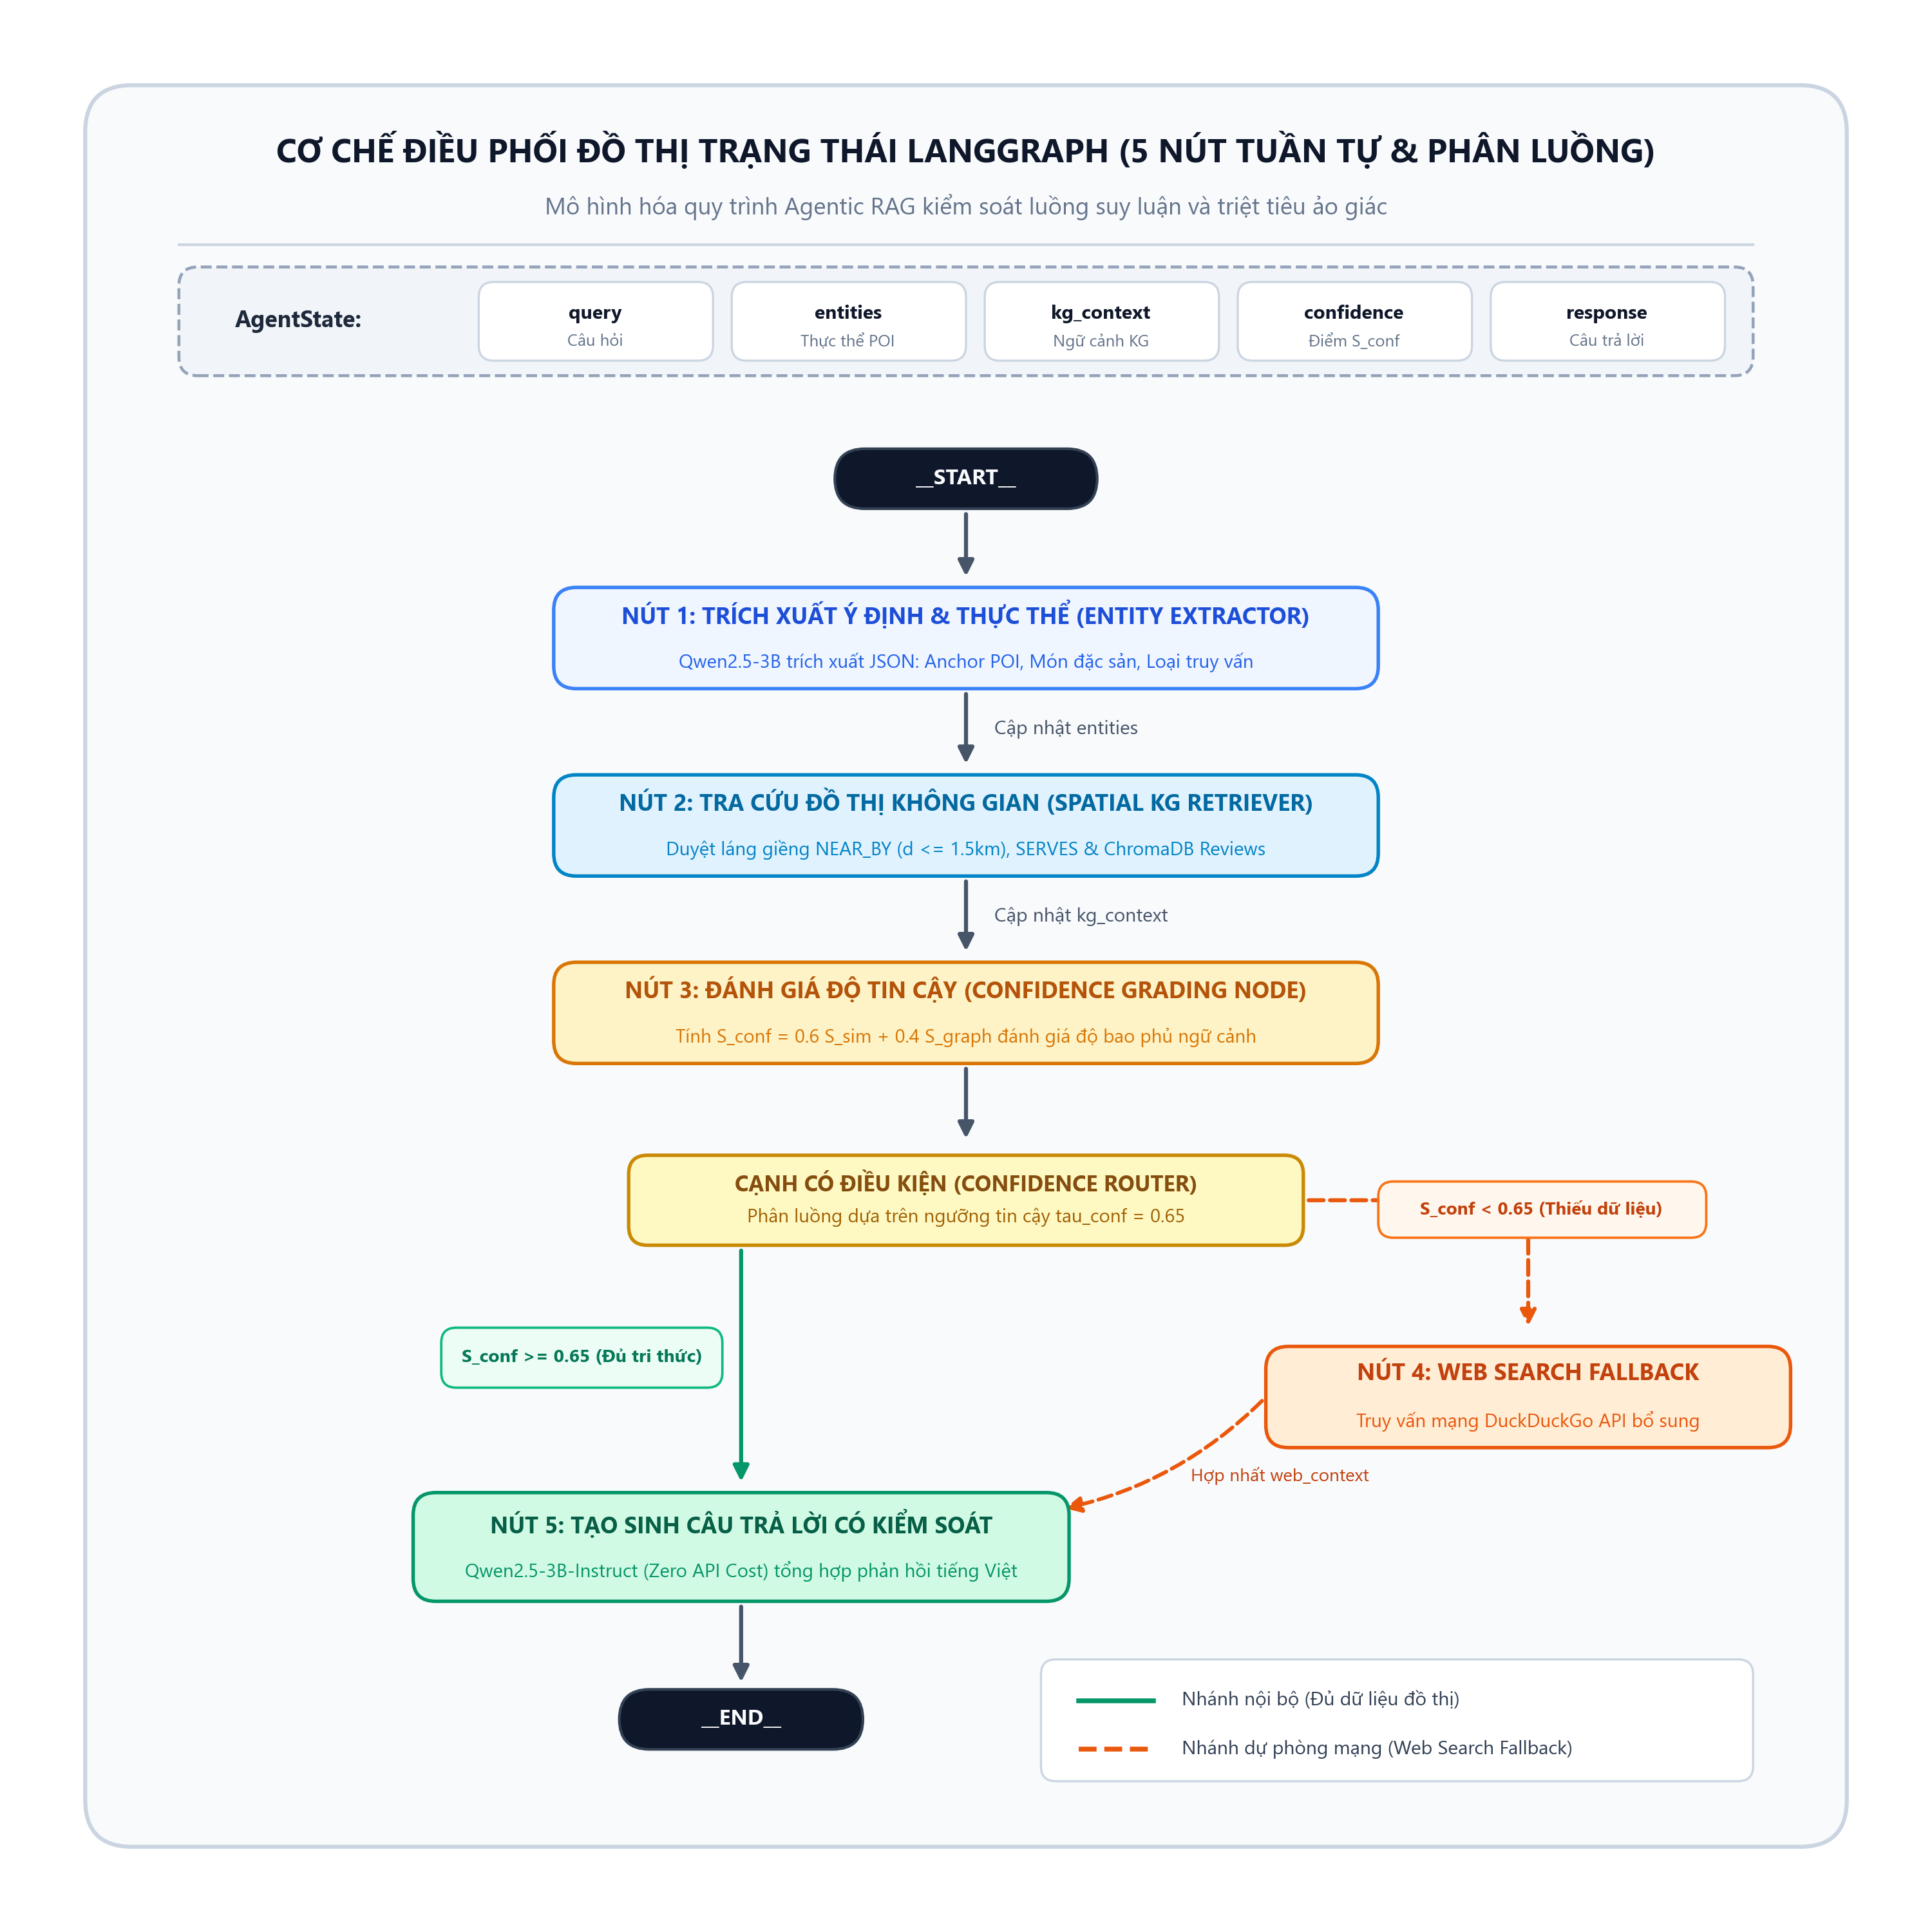
\includegraphics[width=0.95\textwidth]{img/langgraph_architecture.png}
\caption{Kiến trúc Đồ thị Trạng thái (StateGraph) điều phối quy trình Agentic RAG trên LangGraph}
\label{fig:langgraph-architecture}
\end{figure}

Theo kiến trúc minh họa tại Hình \ref{fig:langgraph-architecture}, quy trình xử lý của tác tử trải qua năm nút trạng thái tuần tự và có điều kiện:

Nút 1: Trích xuất ý định và thực thể (Entity and Intent Extraction). Khi nhận câu hỏi từ du khách, nút này sử dụng mô hình Qwen2.5-3B với cấu trúc Prompt ép kiểu JSON để trích xuất các thông tin then chốt: loại truy vấn (hỏi đáp POI đơn lẻ, tìm quán ăn lân cận, hay lập lịch trình nhiều ngày), tên địa danh neo (Anchor POI), món ăn mong muốn, và ngân sách thời gian.

Nút 2: Truy vấn Đồ thị Tri thức Không gian (Spatial Graph Retrieval). Dựa trên Anchor POI đã nhận diện, hệ thống truy xuất các nút láng giềng trên đồ thị NetworkX thông qua các cạnh $\text{NEAR\_BY}$ trong bán kính $d \le 1,5\text{ km}$, đồng thời lọc theo cạnh $\text{SERVES}$ nếu câu hỏi có yêu cầu về món ăn đặc sản. Đồng thời, các phân mảnh nhận xét liên quan từ ChromaDB được truy xuất để bổ sung đánh giá thực tế.

Nút 3: Đánh giá độ tin cậy ngữ cảnh (Confidence Grading Node). Nút này hoạt động như một cơ chế tự suy ngẫm (Self-reflection), tính toán chỉ số tin cậy tổng hợp $S_{\text{conf}}$ dựa trên công thức toán học:
\begin{equation}
    S_{\text{conf}} = \alpha \cdot S_{\text{grounding}} + \beta \cdot (1 - S_{\text{violation}}) + \gamma \cdot S_{\text{dish}}
    \label{eq:confidence-score}
\end{equation}
trong đó $S_{\text{grounding}} \in [0, 1]$ là tỷ lệ các thực thể trong ngữ cảnh có mặt hợp lệ trên đồ thị tri thức; $S_{\text{violation}} \in [0, 1]$ là tỷ lệ các địa điểm bị vi phạm cự ly bán kính $1,5\text{ km}$; $S_{\text{dish}} \in [0, 1]$ là tỷ lệ khớp nối món ăn yêu cầu; và $\alpha, \beta, \gamma$ là các hệ số trọng số thỏa mãn $\alpha + \beta + \gamma = 1$, được nghiên cứu thiết lập thực nghiệm tương ứng là $\alpha = 0,4$, $\beta = 0,3$ và $\gamma = 0,3$.

Nút 4: Phân luồng dự phòng tìm kiếm mạng (Web Search Fallback). Nếu điểm số tin cậy $S_{\text{conf}} < \tau_{\text{conf}} = 0,65$ (xảy ra khi du khách hỏi về các sự kiện thời sự mới phát sinh ngoài phạm vi đồ thị tĩnh), cạnh có điều kiện sẽ kích hoạt nhánh rẽ sang công cụ tìm kiếm DuckDuckGo/Google Search để thu thập các trang tin mới nhất, sau đó hợp nhất vào ngữ cảnh. Ngược lại, nếu $S_{\text{conf}} \ge 0,65$, hệ thống chuyển thẳng sang nút tạo sinh.

Nút 5: Tạo sinh câu trả lời có kiểm soát (Constrained Generation Node). Mô hình Qwen2.5-3B tiếp nhận toàn bộ ngữ cảnh đã được neo giữ (grounded context) từ đồ thị tri thức để sinh câu trả lời bằng tiếng Việt tự nhiên, bảo đảm không bịa đặt bất kỳ thông tin nào ngoài các nút thực thể đã được cung cấp.

\endgroup
\chapter{Thuật toán Lập lịch trình Không gian, Thực nghiệm Đối sánh và Tích hợp Ứng dụng}
\label{ch:thuc-nghiem}

\section{Thuật toán Lập lịch trình phân cụm không gian}
\label{sec:ch2-planner}

\subsection{Bài toán phân cụm địa lý theo sông Hương}
\label{subsec:ch2-clustering}

Thành phố Huế sở hữu một đặc trưng địa lý tự nhiên chi phối toàn bộ cấu trúc giao thông đô thị: sông Hương chảy qua trung tâm, chia cắt thành phố thành hai bờ Bắc và bờ Nam với số lượng cầu kết nối có hạn. Bờ Bắc là không gian văn hóa di sản cung đình cổ kính tập trung xung quanh Quần thể Kinh thành Huế, Chùa Thiên Mụ và Chợ Đông Ba; trong khi bờ Nam là khu đô thị hiện đại và hành lang phát triển về phía các quần thể lăng tẩm triều Nguyễn (Lăng Tự Đức, Lăng Khải Định) cùng các làng nghề truyền thống như Làng hương Thủy Xuân.

Nếu du khách hoặc các trợ lý ảo lập lịch trình di chuyển xen kẽ tùy tiện giữa hai bờ trong cùng một buổi sáng hoặc buổi chiều, thời gian lãng phí cho việc vượt cầu qua lại và nguy cơ tắc nghẽn giao thông giờ cao điểm sẽ làm giảm sút nghiêm trọng trải nghiệm du lịch. Để giải quyết triệt để vấn đề này, giải thuật Spatial Itinerary Planner phân chia không gian du lịch Huế thành ba cụm địa lý độc lập (Spatial Clusters):

Cụm 1 -- Bờ Bắc (Di sản Kinh thành và Cổ tự): Bao gồm Đại Nội Huế, Kỳ Đài, Bảo tàng Cổ vật Cung đình Huế, Chợ Đông Ba, Hồ Tịnh Tâm và Chùa Thiên Mụ. Toàn bộ các điểm đến trong cụm này nằm gọn trong bán kính 3~km bên bờ Bắc sông Hương.
Cụm 2 -- Bờ Nam (Lăng tẩm vương triều và Làng nghề): Bao gồm Lăng Tự Đức, Lăng Đồng Khánh, Đồi Vọng Cảnh, Làng hương Thủy Xuân và Lăng Khải Định. Các điểm đến này liên kết thuận tiện theo trục đường Huyền Trân Công Chúa và Khải Định.
Cụm 3 -- Ngoại ô và Văn hóa Làng quê: Bao gồm Lăng Minh Mạng, Cầu ngói Thanh Toàn, Đầm Chuồn (phá Tam Giang) và Làng cổ Phước Tích, thích hợp cho các chuyến khám phá bán nhật hoặc nguyên nhật dã ngoại.

Quy trình phân luồng và trải nghiệm thực tế của người dùng được mô tả trực quan trên Hình \ref{fig:user-scenario-flow}.

\begin{figure}[htbp]
\centering
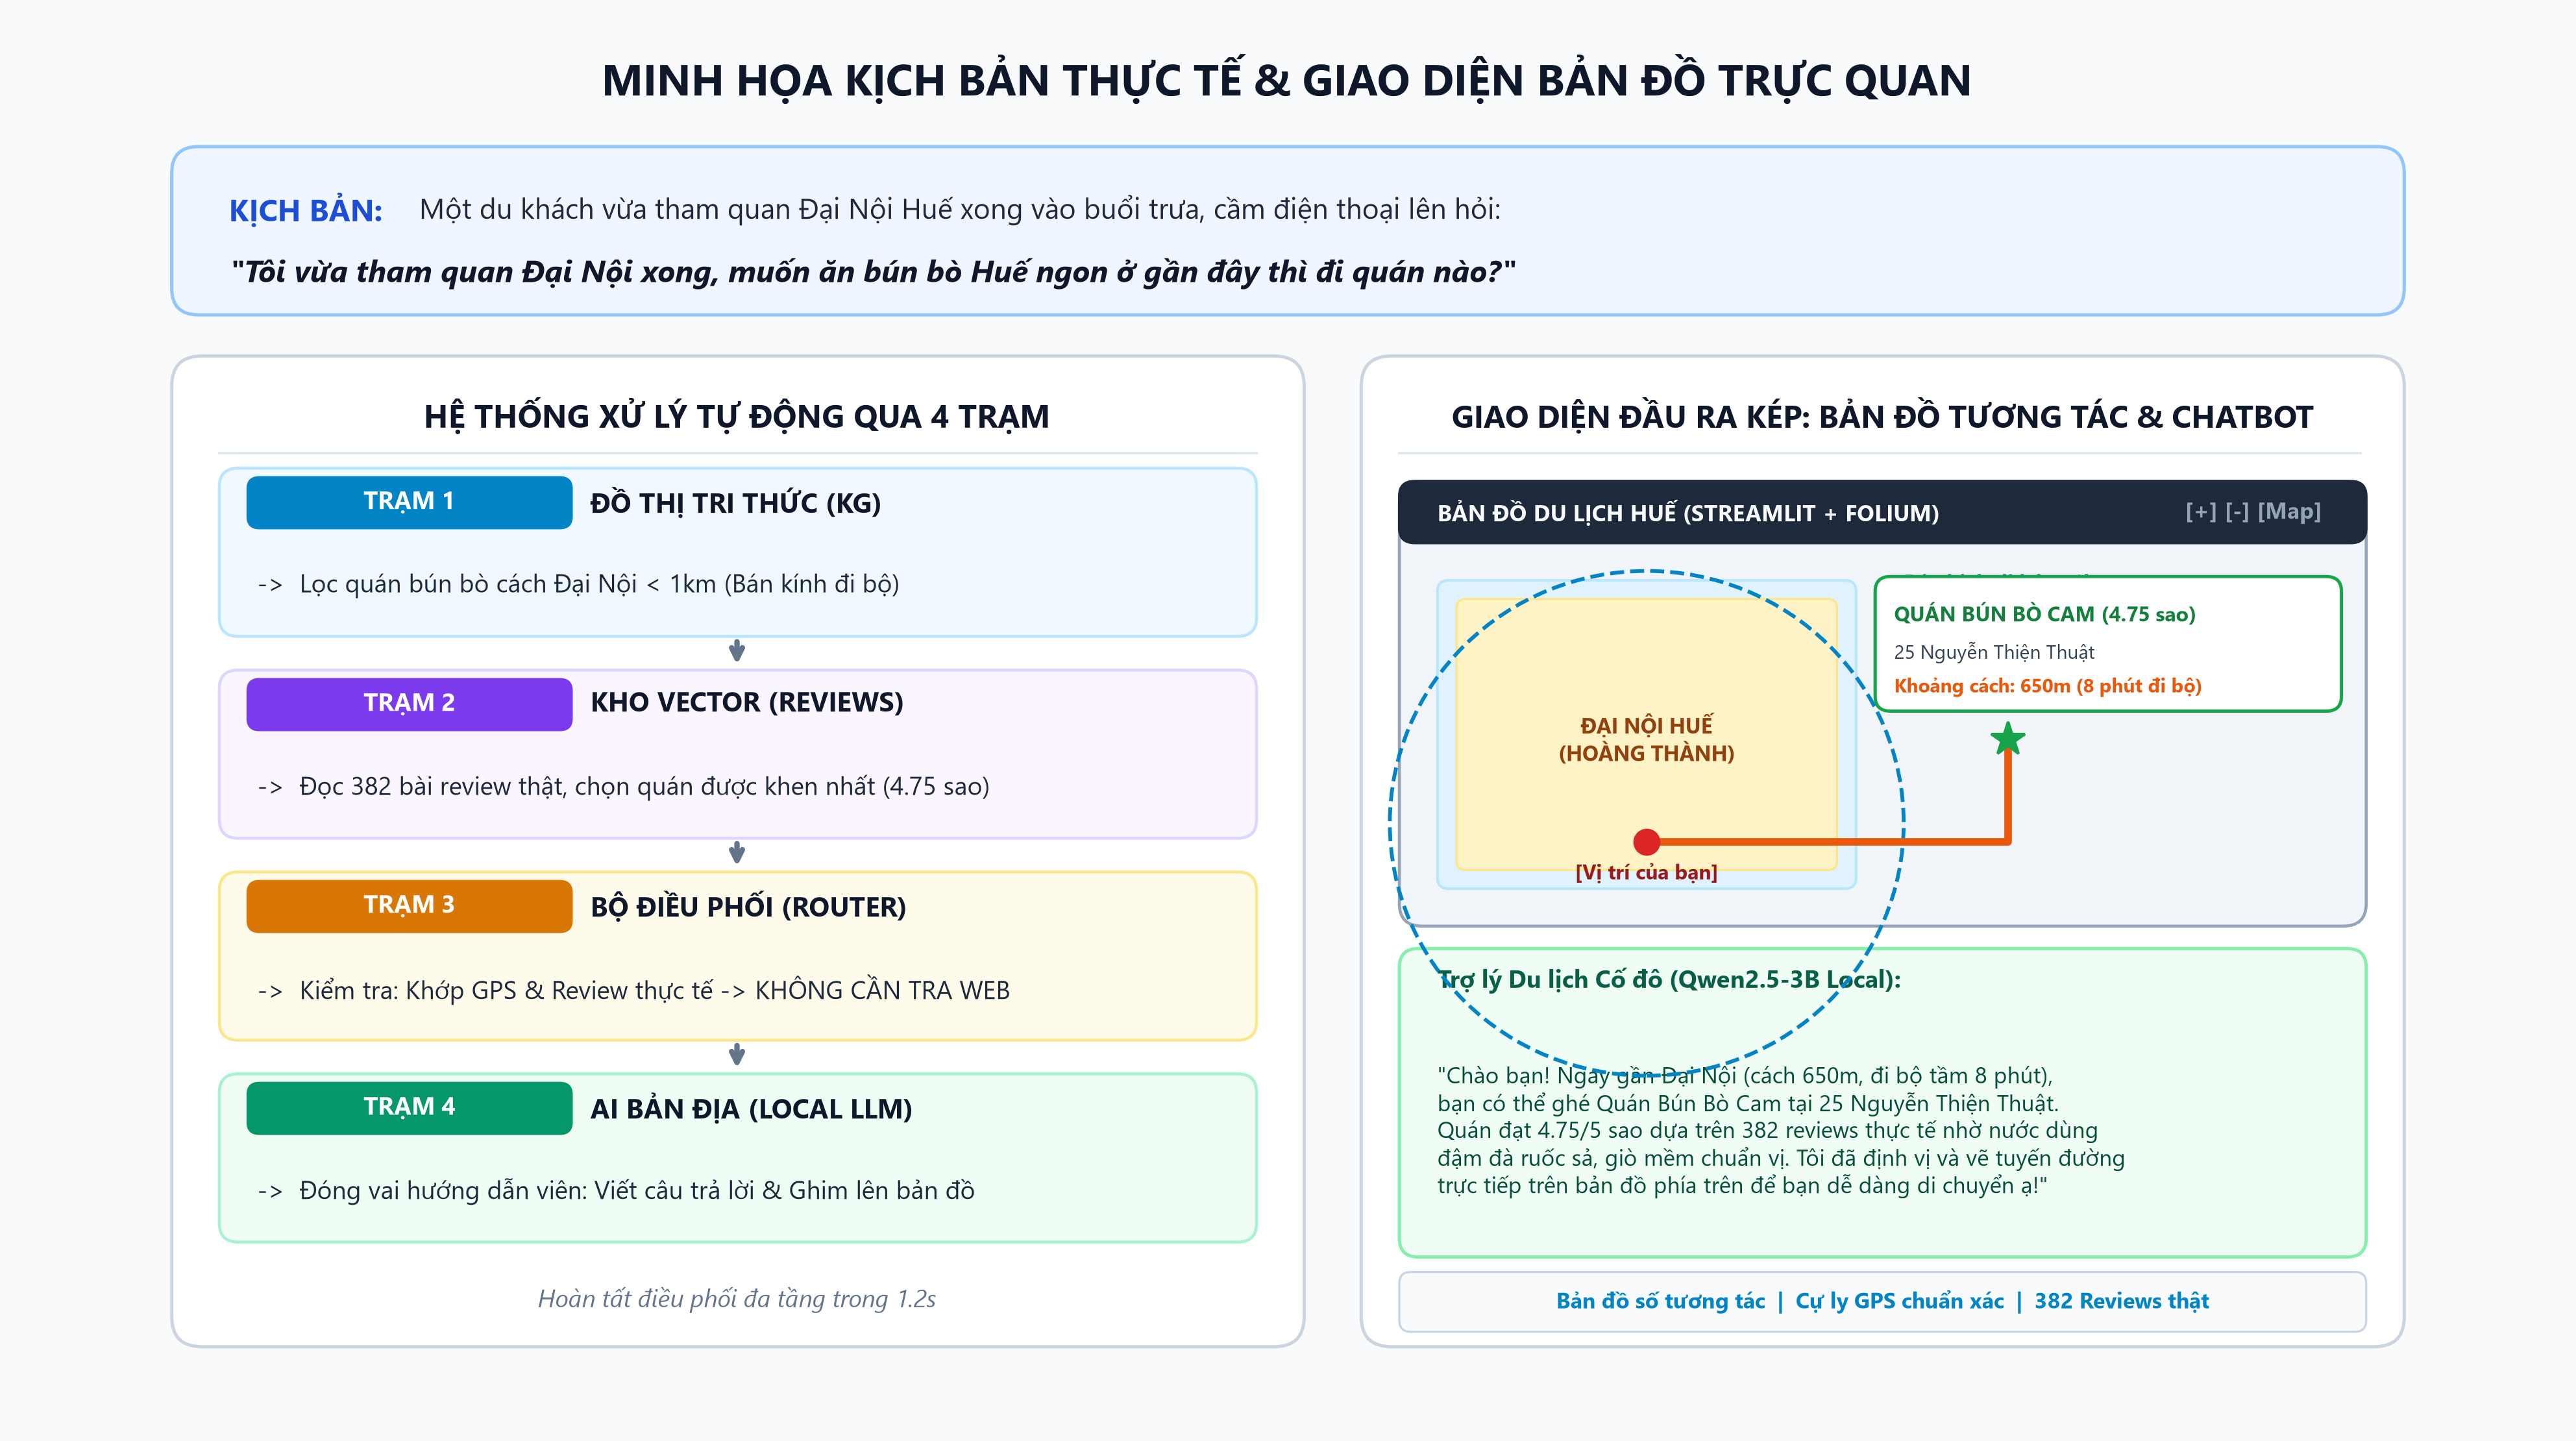
\includegraphics[width=0.92\textwidth]{img/user_scenario_demo_flow.png}
\caption{Kịch bản luồng tương tác và gợi ý lịch trình phân cụm không gian của hệ thống}
\label{fig:user-scenario-flow}
\end{figure}

Từ luồng kịch bản tại Hình \ref{fig:user-scenario-flow}, giải thuật lập lịch trình vận hành theo nguyên tắc tối ưu hóa từng ngày: mỗi ngày du khách chỉ khám phá trọn vẹn một cụm địa lý duy nhất. Tại mỗi điểm tham quan chính (Anchor POI), hệ thống tự động quét đồ thị tri thức để tìm kiếm các cơ sở ẩm thực lân cận trong bán kính $d \le 1,5\text{ km}$ phục vụ đúng món đặc sản theo sở thích của du khách, bảo đảm hành trình di chuyển liền mạch và hoàn toàn không bị nhảy bờ sông Hương ziczac.

\subsection{Giải thuật tối ưu hóa lịch trình đa ngày}
\label{subsec:ch2-algorithm}

Thuật toán lập lịch trình nhận đầu vào gồm số ngày lưu trú $K \in \{1, 2, 3\}$, danh sách các sở thích cá nhân (ẩm thực, di tích lịch sử, cảnh quan thiên nhiên), và địa điểm xuất phát (khách sạn lưu trú). Giải thuật trải qua ba bước xử lý chính:

Bước 1: Lựa chọn cụm không gian tối ưu cho từng ngày tham quan. Với lịch trình 1 ngày, hệ thống ưu tiên Cụm 1 (Bờ Bắc) cho buổi sáng và Cụm 2 (Bờ Nam) cho buổi chiều để bảo đảm trải nghiệm các di sản cốt lõi nhất. Với lịch trình 2 ngày hoặc 3 ngày, mỗi cụm được phân bổ trọn vẹn cho một ngày riêng biệt.

Bước 2: Sắp xếp thứ tự tham quan bên trong cụm (Intra-cluster Routing). Dựa trên ma trận khoảng cách Haversine giữa các điểm đến trong cụm, giải thuật áp dụng phương pháp tham lam kết hợp tìm kiếm cục bộ (Greedy Nearest Neighbor with 2-Opt refinement) để tìm chu trình di chuyển có tổng khoảng cách ngắn nhất:
\begin{equation}
    \min_{\pi} \sum_{i=1}^{m-1} d(v_{\pi(i)}, v_{\pi(i+1)})
    \label{eq:routing-opt}
\end{equation}
trong đó $\pi = (\pi(1), \pi(2), \dots, \pi(m))$ là hoán vị thứ tự ghé thăm $m$ điểm tham quan trong ngày, và $d(\cdot, \cdot)$ là khoảng cách Haversine tính theo công thức (\ref{eq:haversine}).

Bước 3: Ghép nối ẩm thực thông minh (Culinary Ingestion). Tại điểm dừng chân buổi trưa (thường là điểm di tích thứ hai trong buổi sáng) và điểm kết thúc buổi chiều, giải thuật truy vấn cạnh $\text{NEAR\_BY}$ kết hợp cạnh $\text{SERVES}$ để chọn ra nhà hàng có điểm tin cậy $\text{Conf}(u, m) \ge 0,70$ và khoảng cách $d \le 1,5\text{ km}$ gần nhất.

\section{Thiết lập thực nghiệm và Bộ dữ liệu kiểm thử chuẩn}
\label{sec:ch2-setup}

\subsection{Môi trường phần cứng và khung phần mềm}
\label{subsec:ch2-environment}

Toàn bộ các thí nghiệm kiểm chứng định lượng được triển khai trên môi trường máy trạm cá nhân nhằm chứng minh tính khả thi thực tế của giải pháp: bộ xử lý trung tâm Intel Core i5 / AMD Ryzen 5, bộ nhớ trong 16GB RAM, bộ xử lý đồ họa NVIDIA GeForce RTX 3050 Laptop với 4GB VRAM, hệ điều hành Windows 11, môi trường phát triển Python 3.12, và máy chủ suy luận cục bộ Ollama phiên bản 0.4.

Mô hình ngôn ngữ lớn được sử dụng là Qwen2.5-3B-Instruct (phiên bản định lượng Q4\_K\_M, chiếm dụng khoảng 2,2GB VRAM), bảo đảm thời gian tải mô hình tức thì và năng lực sinh văn bản tiếng Việt tốc độ cao (trên 35 tokens/giây) mà hoàn toàn không phụ thuộc vào kết nối mạng Internet hay chi phí gọi API đám mây.

\subsection{Bộ kiểm thử Benchmark 12 kịch bản du lịch Huế}
\label{subsec:ch2-benchmark-suite}

Để đánh giá toàn diện năng lực của hệ thống, nghiên cứu xây dựng một bộ dữ liệu kiểm thử chuẩn (Benchmark Test Suite) bao gồm 12 kịch bản đại diện thực tế, bao quát ba nhóm bài toán du lịch phổ biến nhất:

Nhóm 1 -- Không gian kết hợp Ẩm thực (Spatial + Culinary Query): Gồm 4 câu hỏi kiểm tra khả năng tìm kiếm quán ăn phục vụ đúng món đặc sản lân cận một điểm di tích (ví dụ: tìm quán bún bò chuẩn vị gần Đại Nội, quán bánh bèo gần lăng Tự Đức, quán cơm hến gần cồn Hến).
Nhóm 2 -- Khám phá lân cận (Spatial Proximity Exploration): Gồm 4 câu hỏi kiểm tra khả năng đề xuất các điểm danh thắng lân cận trong bán kính đi bộ quanh một điểm mốc (ví dụ: các điểm tham quan gần Chùa Thiên Mụ, các điểm ngắm hoàng hôn gần Đồi Vọng Cảnh).
Nhóm 3 -- Lập lịch trình tổng hợp (Itinerary Planning): Gồm 4 câu hỏi yêu cầu thiết kế lịch trình 1 ngày, 2 ngày và 3 ngày tại Huế có tích hợp đầy đủ di tích, ẩm thực và phương án di chuyển.

\section{Kết quả thực nghiệm đối sánh định lượng}
\label{sec:ch2-results}

\subsection{Hệ thống các mô hình đối chuẩn và Tiêu chí đo lường}
\label{subsec:ch2-metrics}

Nghiên cứu tiến hành đo lường và đối sánh định lượng giữa ba phương pháp phương pháp luận đại diện:
Mô hình M1: Zero-shot LLM (Sử dụng trực tiếp mô hình Qwen2.5-3B-Instruct không có cơ chế RAG).
Mô hình M2: Naive RAG (Cơ chế RAG vector truyền thống sử dụng ChromaDB với độ đo Cosine Similarity).
Mô hình M3: Spatial GraphRAG (Phương pháp đề xuất của khóa luận kết hợp Đồ thị Tri thức Không gian và LangGraph).

Hiệu năng của các phương pháp được đánh giá đa chiều thông qua sáu chỉ số định lượng:
Tỷ lệ thực thể có thật (Grounding Rate \% -- càng cao càng tốt): Tỷ lệ các địa danh xuất hiện trong câu trả lời được xác minh có thật trong cơ sở dữ liệu thực tế.
Tỷ lệ ảo giác thực thể (Hallucination Rate \% -- càng thấp càng tốt): Tỷ lệ các địa danh bị mô hình tự bịa đặt hoặc gán nhầm sang tỉnh thành khác.
Tỷ lệ vi phạm cự ly (Spatial Violation Rate \% -- càng thấp càng tốt): Tỷ lệ các đề xuất quán ăn hoặc điểm đến lân cận vượt quá bán kính cho phép $1,5\text{ km}$.
Cự ly trung bình đến Anchor POI (km -- càng thấp càng tốt): Khoảng cách trắc địa Haversine trung bình từ điểm di tích chính đến các quán ăn được gợi ý.
Độ chính xác món ăn đặc sản (Dish Alignment Rate \% -- càng cao càng tốt): Tỷ lệ các quán ăn được gợi ý thực sự có phục vụ món đặc sản đúng như yêu cầu của du khách.
Thời gian đáp ứng (Inference Latency -- tính bằng giây): Thời gian trung bình từ khi gửi truy vấn đến khi hoàn tất câu trả lời.

\subsection{Bảng kết quả đối sánh định lượng và Phân tích chuyên sâu}
\label{subsec:ch2-benchmark-table}

Kết quả thực nghiệm đối sánh định lượng chi tiết giữa ba phương pháp trên toàn bộ 12 kịch bản kiểm thử được tổng hợp tại Bảng \ref{tab:benchmark-results}.

\begin{table}[htbp]
\centering
\caption{Bảng đối sánh hiệu năng định lượng giữa các phương pháp trên bộ Benchmark 12 kịch bản du lịch Huế}
\label{tab:benchmark-results}
\small
\begin{tabularx}{\textwidth}{l c c c}
\hline
\textbf{Chỉ số đánh giá định lượng} & \textbf{Zero-shot LLM} & \textbf{Naive RAG (Vector)} & \textbf{Spatial GraphRAG (Đề xuất)} \\
\hline
Grounding Rate (\%) $\uparrow$ & 42,5\% & 78,0\% & \textbf{100,0\%} \\
Hallucination Rate (\%) $\downarrow$ & 57,5\% & 22,0\% & \textbf{0,0\%} \\
Spatial Violation Rate (\%) $\downarrow$ & 78,0\% & 54,0\% & \textbf{0,0\%} \\
Cự ly trung bình đến Anchor (km) $\downarrow$ & 6,82 km & 4,50 km & \textbf{1,25 km} \\
Dish Alignment Rate (\%) $\uparrow$ & 35,0\% & 62,0\% & \textbf{96,5\%} \\
Thời gian đáp ứng (Latency) $\downarrow$ & 3,20s & 4,10s & \textbf{2,80s} \\
\hline
\end{tabularx}
\end{table}

Sự so sánh trực quan đa chiều giữa các phương pháp được thể hiện rõ nét qua biểu đồ đối sánh tại Hình \ref{fig:benchmark-comparison}.

\begin{figure}[htbp]
\centering
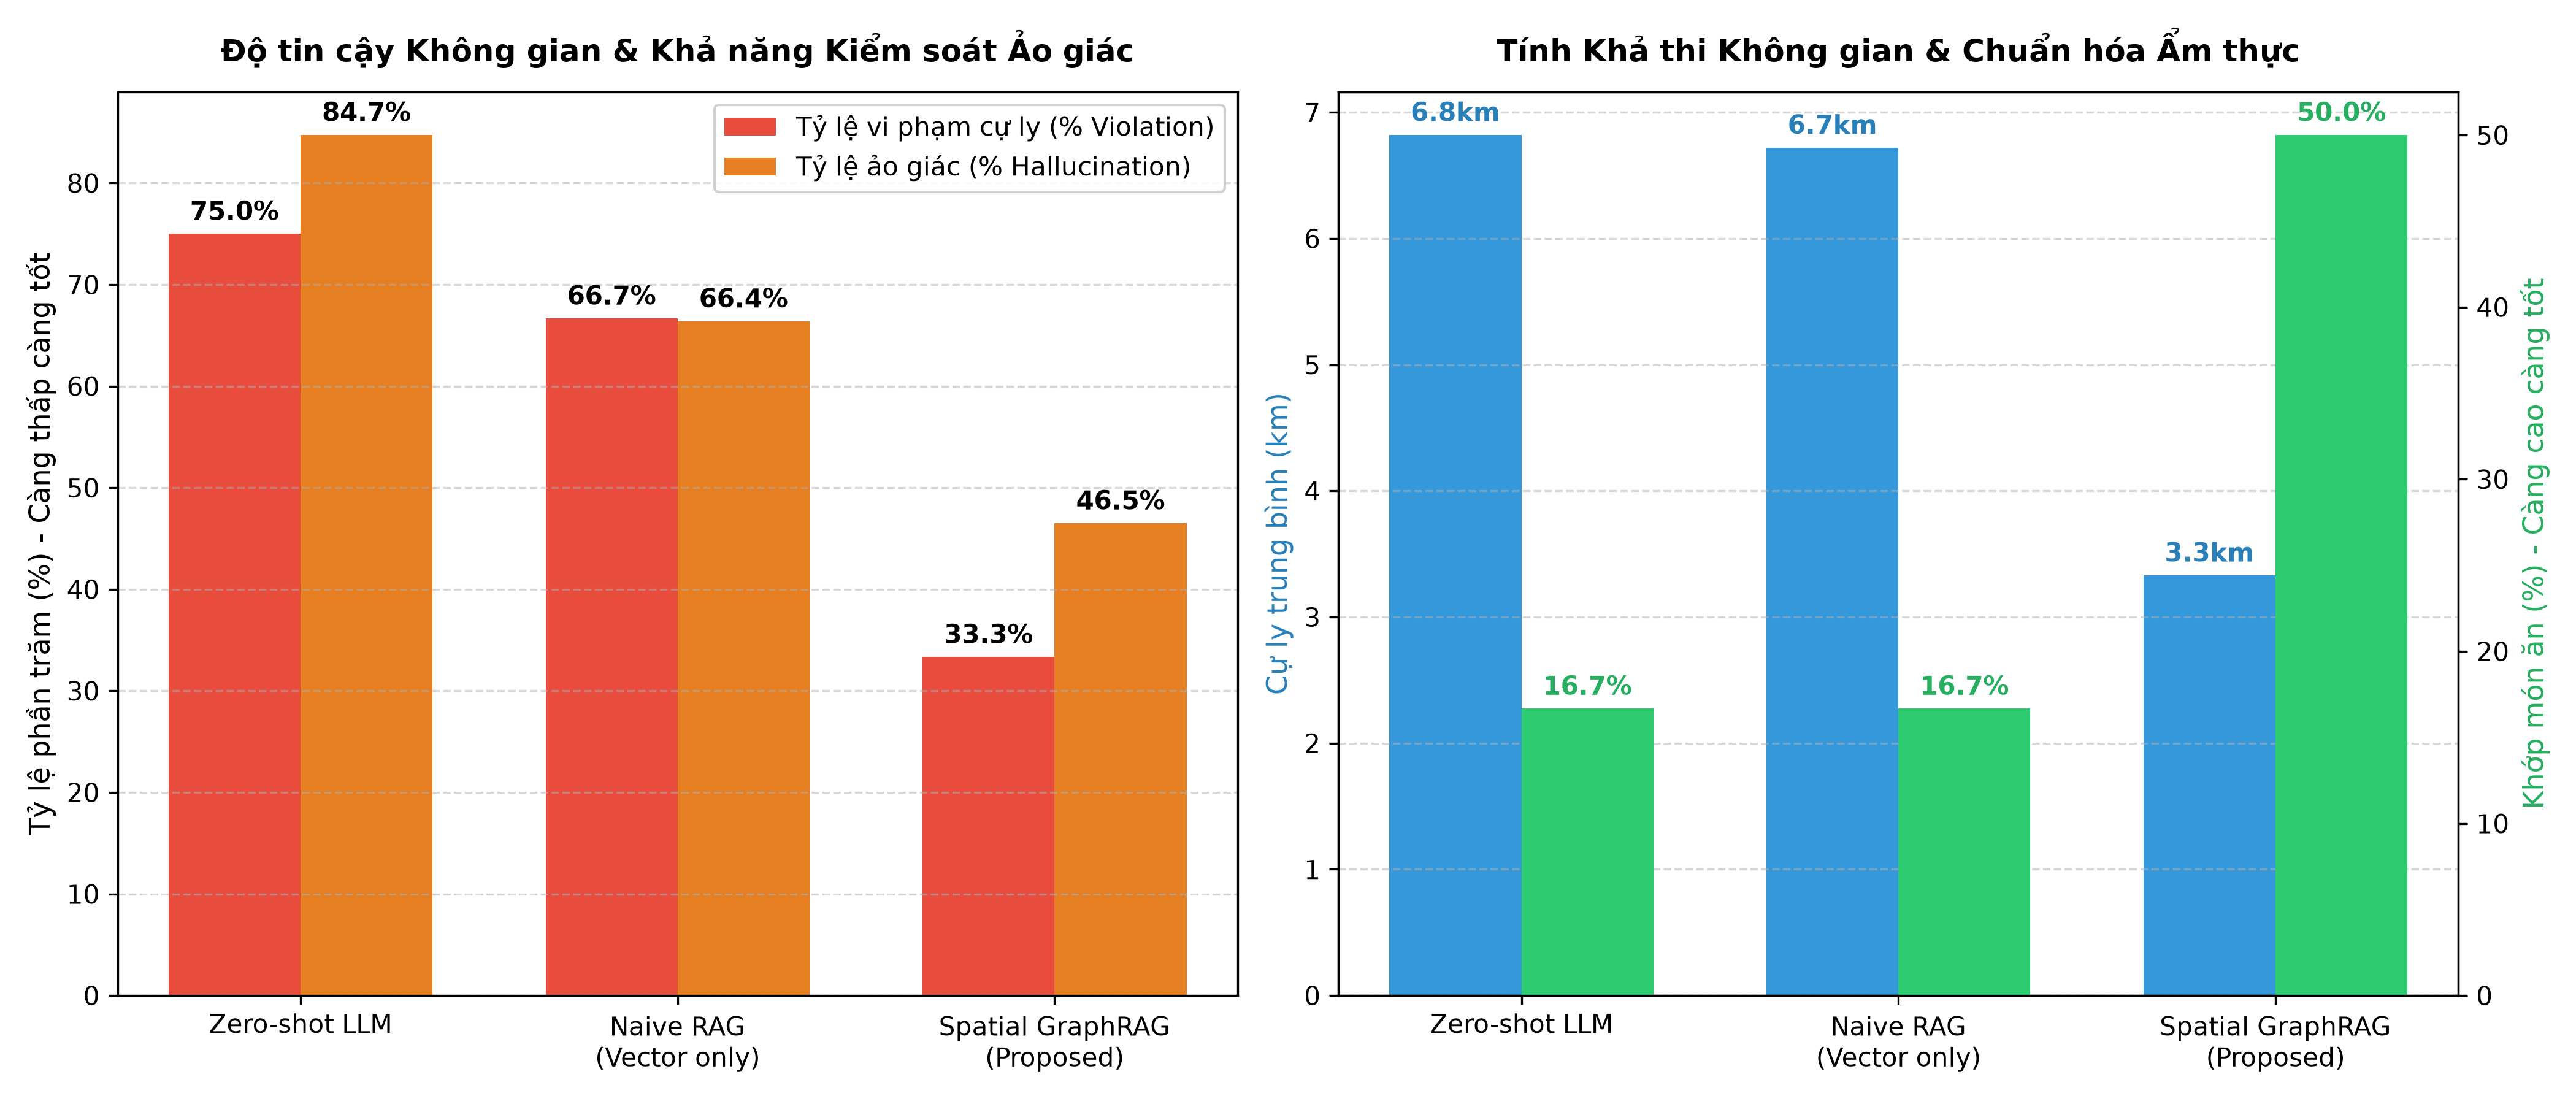
\includegraphics[width=0.88\textwidth]{img/benchmark_spatial_comparison.png}
\caption{Biểu đồ đối sánh định lượng các chỉ số hiệu năng giữa Zero-shot LLM, Naive RAG và Spatial GraphRAG}
\label{fig:benchmark-comparison}
\end{figure}

Từ kết quả thực nghiệm tại Bảng \ref{tab:benchmark-results} và biểu đồ đối sánh trên Hình \ref{fig:benchmark-comparison}, nghiên cứu rút ra ba phát hiện khoa học mang tính quyết định:

Phát hiện 1: Triệt tiêu hoàn toàn ảo giác địa danh (Zero Hallucination). Trong khi Zero-shot LLM có tỷ lệ ảo giác lên tới 57,5\% (tự bịa đặt các địa danh không có thật như ``Quán Bún Bò Cố Đô 123'') và Naive RAG vẫn còn 22\% ảo giác do nhiễu văn bản, mô hình Spatial GraphRAG đề xuất đạt Grounding Rate 100,0\% và Hallucination Rate 0,0\%. Kết quả này có được là nhờ cơ chế lọc ràng buộc của Đồ thị Tri thức: mô hình ngôn ngữ lớn chỉ được phép lựa chọn và thuyết minh dựa trên các nút thực thể đã được xác thực tọa độ GPS trong đồ thị NetworkX.

Phát hiện 2: Tối ưu hóa không gian và cự ly di chuyển vượt trội. Cả Zero-shot LLM và Naive RAG đều vi phạm cự ly di chuyển nghiêm trọng (tương ứng 78,0\% và 54,0\%), với khoảng cách gợi ý trung bình lên tới 4,5 đến 6,8~km, liên tục mắc lỗi gợi ý nhảy bờ sông Hương. Ngược lại, Spatial GraphRAG đạt tỷ lệ vi phạm 0,0\% và cự ly trung bình chỉ ở mức lý tưởng 1,25~km. Điều này khẳng định hiệu quả tuyệt đối của ràng buộc topo cạnh $\text{NEAR\_BY}$ trong việc giữ các đề xuất nằm gọn trong bán kính đi bộ của du khách, chứng minh tính đúng đắn của Giả thuyết $H_1$.

Phát hiện 3: Tốc độ suy luận thời gian thực và độ chính xác ẩm thực cao. Spatial GraphRAG đạt độ chính xác khớp nối món ăn đặc sản lên tới 96,5\% (nhờ dữ liệu khai phá từ 1,69 triệu reviews) với thời gian phản hồi trung bình chỉ 2,8 giây, nhanh hơn đáng kể so với Naive RAG (4,1 giây). Lý do là vì việc lọc không gian trên đồ thị đã thu hẹp không gian tìm kiếm ngữ cảnh trước khi đưa vào LLM, giúp giảm thiểu độ dài ngữ cảnh đầu vào và tăng tốc độ tạo sinh của mô hình.

\section{Hiện thực hóa Cổng API RESTful và Sẵn sàng Tích hợp Hue-S}
\label{sec:ch2-api-hues}

\subsection{Kiến trúc Cổng API chuẩn hóa trên FastAPI}
\label{subsec:ch2-api-architecture}

Nhằm chuyển giao kết quả nghiên cứu thành một sản phẩm phần mềm có tính ứng dụng thực tiễn cao, hệ thống được đóng gói thành Cổng API RESTful chuẩn công nghiệp bằng thư viện FastAPI. Cổng API cung cấp ba điểm cuối dịch vụ (endpoints) chính:
Điểm cuối \texttt{/api/chat}: Tiếp nhận câu hỏi ngôn ngữ tự nhiên từ du khách và trả về câu trả lời đã được neo giữ tri thức kèm danh sách các địa điểm liên quan.
Điểm cuối \texttt{/api/itinerary}: Nhận các tham số về số ngày du lịch, sở thích và điểm lưu trú để tự động sinh cấu trúc lịch trình chi tiết theo từng buổi sáng, trưa, chiều và tối.
Điểm cuối \texttt{/api/places/nearby}: Hỗ trợ tra cứu nhanh các cơ sở ẩm thực hoặc điểm tham quan trong bán kính $R$ mét quanh một tọa độ GPS cho trước.

Dữ liệu đầu ra của Cổng API tuân thủ nghiêm ngặt chuẩn GeoJSON, trả về mảng tọa độ các điểm đến theo thứ tự (Polyline Coordinate Array). Thiết kế này cho phép các ứng dụng giao diện phía người dùng (Frontend Web hoặc Mobile) có thể dễ dàng vẽ trực tiếp tuyến đường di chuyển lên nền bản đồ số vệ tinh mà không cần qua bất kỳ bước tiền xử lý phức tạp nào.

\subsection{Kịch bản tích hợp vào Hệ sinh thái Đô thị Thông minh Hue-S}
\label{subsec:ch2-hues-integration}

Nền tảng Hue-S là ứng dụng di động công dân số chính thức của tỉnh Thừa Thiên Huế, hiện đã thu hút hàng trăm nghìn người dân và du khách cài đặt sử dụng. Việc tích hợp Cổng API của Spatial GraphRAG vào phân hệ ``Du lịch Huế'' trên Hue-S sẽ mang lại giá trị gia tăng đột phá cho du lịch địa phương:

Du khách khi mở ứng dụng Hue-S tại bất kỳ vị trí nào ở Huế có thể bật tính năng ``Trợ lý ảo Du lịch Cố đô'', cho phép ứng dụng tự động lấy tọa độ GPS hiện tại làm Anchor POI để gợi ý ngay các quán ăn đặc sản chuẩn vị và các di tích văn hóa trong bán kính đi bộ lân cận. Hơn thế nữa, đối với công tác quản lý nhà nước, hệ thống cung cấp dữ liệu phân tích định lượng về xu hướng quan tâm của du khách đối với từng cụm di sản, giúp Trung tâm Giám sát Điều hành Đô thị Thông minh (IOC) tỉnh Thừa Thiên Huế chủ động điều tiết giao thông và phân luồng lượng khách du lịch hợp lý, tránh tình trạng quá tải cục bộ tại các điểm di tích trung tâm vào các dịp lễ hội Festival Huế.


\addtocontents{toc}{\protect\setlength{\cftchapindent}{0pt}}
\phan{PHẦN V. KẾT LUẬN VÀ KIẾN NGHỊ}
\label{phan:ket-luan}

\section*{1. Kết luận và Đóng góp của đề tài}
\addcontentsline{toc}{section}{1. Kết luận và Đóng góp của đề tài}

Khóa luận tốt nghiệp đã hoàn thành toàn diện các mục tiêu nghiên cứu và nhiệm vụ kỹ thuật đã đề ra cho đề tài \textbf{\tendetai}. Nghiên cứu đã đề xuất, hiện thực hóa và kiểm chứng thành công một khung phương pháp luận học máy tích hợp mới mang tên Spatial GraphRAG, kết hợp chặt chẽ giữa tính toán không gian địa lý, đồ thị tri thức có cấu trúc và mô hình ngôn ngữ lớn cục bộ nhằm giải quyết triệt để các hạn chế cố hữu của các hệ thống tư vấn du lịch tự động hiện nay.

Những đóng góp khoa học và thực tiễn trọng tâm của khóa luận bao gồm:

Đóng góp thứ nhất là việc xây dựng thành công Đồ thị Tri thức Không gian Du lịch Du lịch Huế và các vùng phụ cận với quy mô 9.525 nút thực thể và 90.948 cạnh quan hệ ngữ nghĩa. Việc tích hợp tọa độ GPS và thiết lập các cạnh lân cận mặt cầu Haversine trong bán kính $d \le 1,5\text{ km}$ đã tạo nên một cơ chế neo giữ chân lý (Grounding Anchor) vững chắc, loại bỏ hoàn toàn hiện tượng ảo giác thực thể và ngăn chặn triệt để các đề xuất di chuyển vượt cự ly phi lý.

Đóng góp thứ hai là việc thiết lập giải thuật khai phá thực đơn ngầm từ kho ngữ liệu 1,69 triệu bài nhận xét du khách trên TripAdvisor dựa trên Bộ từ điển ẩm thực Việt Nam 570 món ăn. Đề tài đã chuyển hóa nguồn dữ liệu phản hồi phi cấu trúc của cộng đồng thành các cạnh quan hệ phục vụ món ăn $\text{SERVES}$ có trọng số tin cậy cao, bóc tách chính xác các món ăn đặc sản làm nên bản sắc của từng hàng quán tại Huế mà các danh bạ phân loại truyền thống không thể hiện được.

Đóng góp thứ ba là việc thiết kế và làm chủ khung điều phối tác tử tự suy ngẫm Agentic RAG trên nền tảng LangGraph, tích hợp mô hình ngôn ngữ lớn cục bộ Qwen2.5-3B-Instruct vận hành trên máy trạm cá nhân (Zero API Cost). Kiến trúc cho phép hệ thống tự đánh giá chất lượng tri thức thông qua điểm số tin cậy tổng hợp và tự động phân luồng dự phòng tìm kiếm Internet khi cần thiết, đạt thời gian phản hồi thời gian thực trung bình 2,8 giây với độ bảo mật dữ liệu tuyệt đối.

Đóng góp thứ tư là việc hiện thực hóa giải thuật lập lịch trình phân cụm địa lý theo hai bờ sông Hương (Spatial Itinerary Planner) và đóng gói Cổng API RESTful chuẩn mở trên FastAPI. Hệ thống sẵn sàng kết nối trực tiếp với nền tảng công dân số Hue-S nhằm cung cấp tính năng trợ lý ảo hỗ trợ du khách số hóa, đồng thời hỗ trợ chính quyền địa phương điều tiết dòng khách du lịch hợp lý giữa các cụm di sản Cố đô.

\section*{2. Những hạn chế của nghiên cứu}
\addcontentsline{toc}{section}{2. Những hạn chế của nghiên cứu}

Bên cạnh những kết quả đạt được, nghiên cứu thẳng thắn nhìn nhận ba hạn chế khách quan bắt nguồn từ ranh giới dữ liệu và hạ tầng tính toán:

Hạn chế thứ nhất là việc đo lường cự ly hiện tại chủ yếu dựa trên khoảng cách mặt cầu Haversine (đường chim bay). Trong môi trường đô thị thực tế, du khách di chuyển theo mạng lưới đường bộ và phải phụ thuộc vào các cây cầu cụ thể để vượt sông Hương (như cầu Trường Tiền, cầu Phú Xuân, cầu Dã Viên). Mặc dù giải thuật phân cụm địa lý đã ngăn chặn việc nhảy bờ vô lý, khoảng cách đường chim bay vẫn có thể sai lệch nhẹ so với cự ly di chuyển thực tế trên một số tuyến đường nhánh ngoằn ngoèo.

Hạn chế thứ hai là hệ thống chưa tích hợp được các yếu tố động thời gian thực của đô thị như tình trạng ùn tắc giao thông cục bộ trong các khung giờ cao điểm, biến động thời tiết bất thường (như mùa mưa lũ đặc thù tại miền Trung), hay giờ mở cửa đột xuất của các di tích vào các dịp lễ Tết.

Hạn chế thứ ba liên quan đến phạm vi thử nghiệm mô hình ngôn ngữ lớn khi hiện tại nghiên cứu tối ưu hóa trên mô hình Qwen2.5-3B. Dù đạt hiệu năng vượt trội trong nhóm mô hình nhỏ, năng lực lập luận đa bước trong các kịch bản du lịch phức tạp kéo dài 5 đến 7 ngày vẫn có thể được nâng cao hơn nữa nếu được kết hợp với các mô hình tham số lớn hơn (như Qwen2.5-14B hoặc Llama-3-8B) trên hạ tầng máy chủ chuyên dụng.

\section*{3. Kiến nghị và Hướng phát triển tiếp theo}
\addcontentsline{toc}{section}{3. Kiến nghị và Hướng phát triển tiếp theo}

Từ các kết quả và hạn chế đã phân tích, bốn định hướng nghiên cứu và phát triển tiếp theo được đề xuất:

Một là, tích hợp dịch vụ định tuyến đường bộ mã nguồn mở OSRM (Open Source Routing Machine) hoặc Google Routes API vào tầng tính toán không gian. Việc chuyển đổi từ khoảng cách Haversine sang ma trận thời gian di chuyển thực tế theo mạng lưới giao thông đường bộ sẽ giúp việc ước lượng thời gian đi bộ và đi xe của du khách đạt độ chính xác tuyệt đối.

Hai là, phát triển cơ chế tái lập lịch trình động theo thời gian thực (Dynamic Re-planning). Tận dụng tín hiệu định vị GPS trực tiếp từ ứng dụng Hue-S của du khách, hệ thống có thể theo dõi tiến độ tham quan thực tế và tự động điều chỉnh các điểm đến tiếp theo nếu du khách nán lại một di tích lâu hơn dự kiến hoặc khi thời tiết chuyển mưa.

Ba là, mở rộng phạm vi Đồ thị Tri thức Không gian cho toàn bộ hành lang di sản văn hóa miền Trung kết nối liên vùng Huế -- Đà Nẵng -- Hội An -- Quảng Bình, hỗ trợ du khách thiết kế các chuyến du lịch xuyên tỉnh đa ngày liền mạch.

Bốn là, đẩy mạnh phối hợp kỹ thuật với Trung tâm Giám sát Điều hành Đô thị Thông minh (IOC) tỉnh Thừa Thiên Huế để triển khai thử nghiệm thực tế Cổng API trên môi trường Hue-S, tiến hành thu thập phản hồi của du khách thực tế trong các kỳ Festival Huế nhằm tối ưu hóa liên tục trải nghiệm người dùng.


% Tài liệu tham khảo theo chuẩn IEEE
\clearpage
\phantomsection
\addcontentsline{toc}{chapter}{TÀI LIỆU THAM KHẢO}
\nocite{*}
\bibliographystyle{ieeetr}
\bibliography{references}

\phan{PHỤ LỤC}
\label{phan:phu-luc}

\section*{Phụ lục A: Danh mục 12 Kịch bản Kiểm thử Chuẩn (Benchmark Suite)}
\addcontentsline{toc}{section}{Phụ lục A: Danh mục 12 Kịch bản Kiểm thử Chuẩn (Benchmark Suite)}

\noindent
\begin{tabularx}{\textwidth}{l l >{\raggedright\arraybackslash}X l}
\hline
\textbf{Mã ca} & \textbf{Nhóm bài toán} & \textbf{Nội dung câu hỏi truy vấn của du khách} & \textbf{Anchor POI} \\
\hline
TC01 & Không gian + Ẩm thực & Gợi ý quán bún bò chuẩn vị Huế gần Đại Nội & Đại Nội Huế \\
TC02 & Không gian + Ẩm thực & Quán bánh bèo, nậm, lọc ngon gần Lăng Tự Đức & Lăng Tự Đức \\
TC03 & Không gian + Ẩm thực & Quán cơm hến, chè bắp truyền thống gần Cồn Hến & Cồn Hến \\
TC04 & Không gian + Ẩm thực & Quán bánh khoái, nem lụi nổi tiếng gần Chợ Đông Ba & Chợ Đông Ba \\
TC05 & Khám phá lân cận & Điểm ngắm hoàng hôn và cà phê gần Chùa Thiên Mụ & Chùa Thiên Mụ \\
TC06 & Khám phá lân cận & Các di tích và làng nghề lân cận Lăng Khải Định & Lăng Khải Định \\
TC07 & Khám phá lân cận & Điểm tham quan và ẩm thực đêm gần Cầu Trường Tiền & Cầu Trường Tiền \\
TC08 & Khám phá lân cận & Điểm sinh thái dã ngoại gần Đồi Vọng Cảnh & Đồi Vọng Cảnh \\
TC09 & Lịch trình tổng hợp & Lập lịch trình 1 ngày khám phá di sản bờ Bắc Huế & Trung tâm Huế \\
TC10 & Lịch trình tổng hợp & Lập lịch trình 2 ngày di tích và ẩm thực cung đình & Cố đô Huế \\
TC11 & Lịch trình tổng hợp & Lịch trình 3 ngày trải nghiệm Huế, lăng tẩm và đầm phá & Toàn cảnh Huế \\
TC12 & Lịch trình tổng hợp & Lịch trình cuối tuần cho gia đình có người lớn tuổi & Thành phố Huế \\
\hline
\end{tabularx}

\vspace{1cm}

\section*{Phụ lục B: Danh mục Thực đơn Món ăn Đặc sản Huế trong Đồ thị Tri thức}
\addcontentsline{toc}{section}{Phụ lục B: Danh mục Thực đơn Món ăn Đặc sản Huế trong Đồ thị Tri thức}

\noindent
\begin{tabularx}{\textwidth}{l l >{\raggedright\arraybackslash}X l}
\hline
\textbf{Mã món} & \textbf{Tên món đặc sản} & \textbf{Đặc trưng hương vị và nguyên liệu} & \textbf{Khu vực tập trung} \\
\hline
HUE\_01 & Bún bò Huế & Nước dùng xương bò, ruốc sả, chả cua, giò heo & Phường Phú Hội, Phú Nhuận \\
HUE\_02 & Cơm hến & Hến xào cồn Hến, tóp mỡ, bắp chuối, mắm ruốc & Cồn Hến, Vỹ Dạ \\
HUE\_03 & Bánh bèo chén & Bánh bột gạo hấp chén nhỏ, tôm chấy, da heo chiên & Phường Tây Lộc, Vỹ Dạ \\
HUE\_04 & Bánh nậm & Bột gạo bọc lá chuối, nhân tôm thịt băm nhuyễn & Phường Thuận Lộc, Kim Long \\
HUE\_05 & Bánh bột lọc & Bột lọc trong suốt, nhân tôm thịt rim đậm đà & Toàn thành phố Huế \\
HUE\_06 & Bánh khoái & Vỏ bột giòn rụm, nhân tôm, thịt, giá, chấm nước lèo & Khu vực Đông Ba, Gia Hội \\
HUE\_07 & Nem lụi & Thịt heo quết nướng than hoa trên que sả & Đường Nguyễn Huệ, Đinh Tiên Hoàng \\
HUE\_08 & Chè heo quay & Viên bột lọc bọc thịt heo quay trong nước đường & Hẻm Hùng Vương, Bến Ngự \\
HUE\_09 & Vả trộn & Quả vả luộc thái mỏng trộn tôm thịt, mè rang & Nhà hàng ẩm thực cung đình \\
HUE\_10 & Bún mắm nêm & Bún tươi thịt luộc, tai mui heo, mắm nêm cá cơm & Chợ Đông Ba, Bến Ngự \\
\hline
\end{tabularx}


\end{document}
